\chapter{Functions}
\section*{Introduction}
In this chapter I give basic usage information for the functions included in the JVSIP implementation of the C VSIPL specification and also related information for the \pyjv{} python module.  I only include functions implemented in \jv{}; either in the C VSIPL library or the \pyjv{} module. Functions covered in the C specification not (currently) supported in \ttbf{JVSIP} are not covered in this manual.

Usage information may also be found by reading the C VSIPL specification, either the old one included with the JVSIP distribution or the newer one developed by the HPEC working group of the OMG.  I currently recommend sticking with the old one included with the JVSIP distribution.  There is a lot of information about C VSIPL in the specification so C VSIPL information in this document will not be extensive; and since \pyjv{}	 has no specification document I will spend more time covering the \pyjv{} methodology.

I try and include information on the \pyjv{} methods and functions collocated with the corresponding C VSIPL information.  Reading the pyJvsip.py module file is also encouraged.  \ttbf{PyJvsip} includes some functionality not (directly) part of C VSIPL.  I will try and highlight these special cases.  

For python information the python help mechanism has also been supported somewhat; but keeping that information correct, up-to-date, and available for every function is a work in progress. 

Keep in mind this chapters main purpose is as a go-to reference for proper incantations when writing code. Except for the introductory sections it is probably not something you will want to read.

In order to have some reasonable ordering of the functions the alphabetical listing is based upon a root function name, not the actual vsip function. For instance the second function in the list is the \ilCode{add} function. There are several \ilCode{add} functions in the Core profile. All of them are placed together under \ilCode{add}.

When a C VSIPL function requires a special object it needs support functions to create the object, and destroy it, and perhaps query it for its attributes. For instance to do a discrete Fourier transform one needs a function to create an FFT object, a function to do the actual FFT using the FFT object, and a function to destroy the FFT object when it is no longer needed. The author calls functions which are designed to work together to do a single job function sets. Function sets are placed together under a single heading. For instance all the functions involved with doing an FFT are placed under the FFT heading.

As discussed in chapter one python supports polymorphism, and object oriented programing. A \pyjv{} object is an instantiation of a python class definition. The python object will contain a C VSIPL object as an instance variable as well as other information needed by \pyjv. For this reason the python garbage collector will destroy C VSIPL objects when no reference to the \pyjv{} object exists.

Because of the true object oriented nature of \pyjv{} there are methods defined for every class which accomplish most of the functionality of C VSIPL. \ttbf{PyJvsip} also defines many functions which operate on the \pyjv{} objects. Frequently you can use either a method or a function. This information is reflected in the JVSIP function list.

No attempt is made to be exhaustive in the function descriptions. Those interested in more detail are directed to the VSIPL specification document included with the \jv{} distribution. In addition various examples included in this document will provide more detail on the use of some of the more complicated functions.
%
\section*{C VSIPL Specification}\addcontentsline{toc}{section}{C VSIPL Specification}
The main document on which \ttbf{JVSIP} is based is the \emph{VSIPL 1.3 API} as approved by the VSIPL Forum on January 31, 2008.  That document is included with the \ttbf{JVSIP} distribution.  The main purpose of this section is to provide a roadmap for people who are familiar with the C VSIPL specification to get around in this \ttbf{JVSIP} manual.  Here I provide tables in an order matching the \emph{VSIPL 1.3 API} specification with links to the same information as presented  in the \ttbf{JVSIP} manual.
\begin{table}[H]
\hypertarget{VSIPspecHead}{}
\caption{VSIPL Specification Chapters}
\label{tab:vsiplAPI}
\begin{center}
\begin{tabular}{l}
VSIPL INTRODUCTION\\
SUMMARY OF VSIPL TYPES\\
\hyperlink{vsiplAPISupport}{SUPPORT FUNCTIONS}\\
\hyperlink{ScalarFunctions}{SCALAR FUNCTIONS}\\
\hyperlink{Random}{RANDOM NUMBER GENERATION}\\
\hyperlink{vectorAndElementwise}{VECTOR \& ELEMENTWISE OPERATIONS}\\
\hyperlink{vsiplSignalProcessing}{SIGNAL PROCESSING FUNCTIONS}\\
\hyperlink{linearAlgebraFunctions}{LINEAR ALGEBRA FUNCTIONS}\\
\hyperlink{Addendum}{VSIPL Addendum}\\
\end{tabular}
\end{center}
\label{default}
\end{table}%
%%
      \subsection*{Summary of VSIPL Types\hspace*{\fill}\hyperlink{VSIPspecHead}{(up)}}\addcontentsline{toc}{subsection}{Summary of VSIPL Types}

%%
   \subsection*{Support Functions\hypertarget{supportFunctions}{} \hspace*{\fill}\hyperlink{VSIPspecHead}{(up)}}\addcontentsline{toc}{subsection}{Support Functions}
\begin{table}[H]
\hypertarget{vsiplAPISupport}{}
\caption{Support Function Overview}
\label{tab:vsiplAPISupport}
\begin{center}
\begin{tabular}{l}
Initialization \ref{tab:initSupport}\\
Array and Block Object Functions \ref{tab:blockSupport}\\
View Object Functions \ref{tab:viewSupport}\\
\end{tabular}
\end{center}
\label{default}
\end{table}%
%%%
     \begin{table}[H]
\caption{Initialization \ref{tab:vsiplAPISupport}}
\label{tab:initSupport}
\begin{center}
\begin{tabular}{|l|l|}\hline
\hlnkFunc{init} & Initialize the VSIP Library\\
\hlnkFunc{finalize} & Finalize the VSIP Library\\
\hline\end{tabular}
\end{center}
\label{default}
\end{table}%
 %table of
     \begin{table}[H]
\caption{Array and Block Object Functions}
\label{tab:blockSupport}
\begin{center}
\begin{tabular}{|l|l|}
\hlnkFunc{init} & Initialize the VSIP Library\\
\hlnkFunc{finalize} & Finalize the VSIP Library\\
\end{tabular}
\end{center}
\label{default}
\end{table}%
 % table of
     \subsubsection*{View Objects\hypertarget{ViewObjects}{}\hspace*{\fill}\hyperlink{supportFunctions}{(up)}}\addcontentsline{toc}{subsubsection}{View Class}
\begin{table}[H]
\caption{View Support}
\label{tab:viewSupport}
\begin{center}
\begin{tabular}{|l|l|}\hline
\hlnkFunc{alldestroy} & Free both \ttbf{block} and \ttbf{view}.\\
\hlnkFunc{bind} & Bind a \ttbf{view} to a \ttbf{block}.\\
\hlnkFunc{cloneview} & Clone a \ttbf{view}.\\
\hlnkFunc{colview} & Return a column \ttbf{view} (vector) of a matrix \ttbf{view}\\
\hlnkFunc{create} & Create a \ttbf{view}.\\
\hlnkFunc{destroy} & Free a \ttbf{view}.\\
\hlnkFunc{get} & Get a value from a \ttbf{view}\\
\hlnkFunc{getblock} & Return \ttbf{block} associated with \ttbf{view}\\
\hlnkFunc{getattrib} & Get attribute structure associated with \ttbf{view}\\
\hlnkFunc{getlength} & Get get length of vector \ttbf{view}\\
\hlnkFunc{getcollength} & Get length of matrix \ttbf{view} column\\
\hlnkFunc{getrowlength} & Get length of matrix \ttbf{view} row\\
\hlnkFunc{getoffset} & Get get offset into block of vector \ttbf{view}\\
\hlnkFunc{getstride} & Get stride through block of vector \ttbf{view}\\
\hlnkFunc{getcolstride} & Get stride through block of matrix \ttbf{view} for columns.\\
\hlnkFunc{getrowstride} & Get stride through block of matrix \ttbf{view} for rows.\\
\hlnkFunc{getxlength} & Get get X length of tensor \ttbf{view}\\
\hlnkFunc{getxstride} & Get the X stride attribute of a tensor \ttbf{view}\\
\hlnkFunc{getylength} & Get get Y length of tensor \ttbf{view}\\
\hlnkFunc{getystride} & Get the Y stride attribute of a tensor \ttbf{view}\\
\hlnkFunc{getzlength} & Get get Z length of tensor \ttbf{view}\\
\hlnkFunc{getzstride} & Get the Z stride attribute of a tensor \ttbf{view}\\
\hlnkFunc{imagview} & Return \ttbf{view} of imaginary part of complex \ttbf{view}\\
\hlnkFunc{matrixview} & Create a matrix view of a 2-D slice of the tensor \ttbf{view}\\
\hlnkFunc{put} & Get a value from a \ttbf{view}\\
\hlnkFunc{putattrib} & Set attribute structure associated with \ttbf{view}.\\
\hlnkFunc{putlength} & Set length of vector \ttbf{view}.\\
\hlnkFunc{putcollength} & Set length of matrix \ttbf{view} column.\\
\hlnkFunc{putrowlength} & Set length of matrix \ttbf{view} row.\\
\hlnkFunc{putoffset} & Set offset into block of vector \ttbf{view}.\\
\hlnkFunc{putstride} & Set stride through block of vector\ttbf{view}.\\
\hlnkFunc{putcolstride} & Set stride through block of matrix \ttbf{view} column.\\
\hlnkFunc{putrowstride} & Set stride through block of matrix \ttbf{view} row.\\
\hlnkFunc{putxlength} & Set X length of tensor \ttbf{view}\\
\hlnkFunc{putxstride} & Set X stride through block of tensor\ttbf{view}\\
\hlnkFunc{putylength} & Set Y length of tensor \ttbf{view}\\
\hlnkFunc{putystride} & Set Y stride through block of tensor\ttbf{view}\\
\hlnkFunc{putzlength} & Set Z length of tensor \ttbf{view}\\
\hlnkFunc{putzstride} & Set Z stride through block of tensor\ttbf{view}\\
\hlnkFunc{realview} & Return \ttbf{view} of real part of complex \ttbf{view}.\\
\hlnkFunc{rowview} & Return a row \ttbf{view} (vector) of a matrix \ttbf{view}\\
\hlnkFunc{subview} & Create a sub-\ttbf{view} of a \ttbf{view}.\\
\hlnkFunc{transview} & Create a matrix \ttbf{view} as a transpose of a matrix\ttbf{view}\\
\hlnkFunc{vectview} & Create a vector \ttbf{view} of a 1-D slice of a tensor \ttbf{view}\\
\hline\end{tabular}
\end{center}
%\label{default}
\end{table}%

%%
   \subsection*{Scalar Functions}\addcontentsline{toc}{subsection}{Scalar Functions}
In general I do not define scalar functions in \pyjv.  Ease of use is a major goal of the \pyjv{} module and to further this goal I decided scalars used by or returned by \pyjv{} functions should be normal python scalars. Using scalar functions (such as $\cos$, $\sin$, etc.) imported from the math module or the numpy module should work fine. That said, you can always use the C VSIPL scalar functions directly since they are in the \ttbf{vsip} module which is included in the \pyjv{} module.
%%
   \subsection*{Random Number Generation \hyperlink{VSIPspecHead}{(up)}\hypertarget{Random}{}}\addcontentsline{toc}{subsection}{Random Number Generation}
VSIPL supports a pseudo random number generator which may be used to produce either a normal random number or a uniform random number. The C VSIPL specification has a particular random number generator defined so that it will produce the same numbers independent of the implementation. This is called a portable random number generator and is indicated during the creation of the random number state object with a flag \ttbf{VSIP\_PRNG}. The specification also supports an implementation dependent randomnumber generator using the flag \ttbf{VSIP\_NPRNG}.\\
\begin{table}[h]
\centering
\begin{tabular}{|l|l|}
\multicolumn{2}{c}{\hyperlink{randomNumbers}{Random Numbers Function Set}}\\
\hline
randcreate & Create a random number object with initial state\\
randdestroy & Destroy a random number object\\
randu & Fill a \ttbf{view} with uniform random numbers\\
randn & Fill a \ttbf{view} with normal random numbers\\
\hline
\end{tabular}
\end{table}
%%
   \subsection*{Elementwise Operations
\hspace*{\fill}\hyperlink{VSIPspecHead}{(up)}\hypertarget{ElementwiseOperations}{}} \addcontentsline{toc}{subsection}{Elementwise Operations}
Elementwise operatons are simple operations which are done on each element in a matrix or vector. Most of the time, when more than one \ttbf{view} is input, the \ttbf{view} shapes will need to be the same since the operation is done to identically indexed elements for each input \ttbf{view} and the operation result is placed in an identically indexed element of the output \ttbf{view}. \\
The tables referenced in this section list elementwise operations with a link to the corresponding function page. Although the function pages are alphabetical, the lists here are in the same order (although not necessarily identical) to the order they appear in the C VSIPL specification.\\
\begin{table}[H]
\hypertarget{vectorAndElementwise}{}
\caption{Vector And Elementwise Operations}
\label{tab:elementwiseChapter}
\begin{center}
\begin{tabular}{|l|}\hline
\hyperlink{elementaryMath}{Elementary Math Functions}\\
\hyperlink{unaryOperations}{Unary Operations}\\
\hyperlink{binaryOperations}{Binary Operations}\\
\hyperlink{ternaryOperations}{Ternary Operations}\\
\hyperlink{logicalOperations}{Logical Operations}\\
\hyperlink{selectionOperations}{Selection Operations}\\
\hyperlink{bitwiseOperators}{Bitwise and Boolean Logical Operators}\\
\hyperlink{elementGenerationOperations}{Element Generation and Copy}\\
\hyperlink{manipulationOperations}{Manipulation Operations}\\
\hline\end{tabular}
\end{center}
\label{default}
\end{table}%
%%%
      \subsubsection*{Elementary Math}\addcontentsline{toc}{subsubsection}{Elementary Math}
Elementary math functions constitute elementwise applications of elementary operations on \ttbf{view}s. The term \emph{elementary} is somewhat arbitrary but includes trigonometric functions, log functions, and exponential functions. Functions here (for elements) are defined by C 89 in the \ttbf{math.h} header file. \ttbf{JVSIP} generally uses this math library to do the calculations for these functions.
\begin{table}[H]
\caption{Elementary Math Functions\ref{tab:elementwiseChapter}}
\label{tab:elementaryMath}
\begin{center}
\begin{tabular}{|l|l|}
\hlnkFunc{acos} & Arccosine\\
\hlnkFunc{asin} & Arcsine\\
\hlnkFunc{atan} & Arctangent\\
\hlnkFunc{atan2} & Arctangent of Two Arguments\\
\hlnkFunc{cos} & Cosine\\
\hlnkFunc{cosh} & Hyperbolic Cosine\\
\hlnkFunc{exp} & Exponential\\
\hlnkFunc{exp10} & Exponential Base 10\\
\hlnkFunc{log} & Natural Log\\
\hlnkFunc{log10} & Base 10 Log\\
\hlnkFunc{sin} & Sine \\
\hlnkFunc{sinh} & Hyperbolic Sine\\
\hlnkFunc{sqrt} & Square Root\\
\hlnkFunc{tan} & Tangent\\
\hlnkFunc{tanh} & Hyperbolic Tangent\\
\end{tabular}
\end{center}
\label{default}
\end{table}%

      \subsubsection*{Unary Operations\hspace*{\fill}\hyperlink{ElementwiseOperations}{(up)}\hypertarget{unaryOperations}{}}\addcontentsline{toc}{subsubsection}{Unary Operations}
Unary operations involve calculations on a single \ttbf{view}. Functions which involve a calculation where the answer is a scalar, such as \ttbf{sumval} generally have a \ttbf{val} as part of the root name. 
\begin{table}[H]
\caption{Unary Operations}
\label{tab:unaryOperations}
\begin{center}
\begin{tabular}{|l|l|}\hline
\hlnkFunc{arg} & Argument\\
\hlnkFunc{ceil} & Ceiling\\
\hlnkFunc{conj} & Conjugate\\
\hlnkFunc{cumsum} & Cumulative Sum\\
\hlnkFunc{euler} & Euler\\
\hlnkFunc{floor} & Floor\\
\hlnkFunc{mag} & Magnitude\\
\hlnkFunc{cmagsq} & Complex Magnitude Squared\\
\hlnkFunc{meanval} & Mean Value\\
\hlnkFunc{meansqval} & Mean Square Value\\
\hlnkFunc{modulate} & Modulate\\
\hlnkFunc{neg} & Negate\\
\hlnkFunc{recip} & Reciprocal\\
\hlnkFunc{round} & Round\\
\hlnkFunc{rsqrt} & reciprocal Square Root\\
\hlnkFunc{sq} & Square\\
\hlnkFunc{sumval} & Sum Value\\
\hlnkFunc{sumsqval} & Sum of Squares Value\\
\hline\end{tabular}
\end{center}
%\label{default}
\end{table}%

      \subsubsection*{Binary Operations\hspace*{\fill}\hyperlink{ElementwiseOperations}{(up)}\hypertarget{binaryOperations}{}}\addcontentsline{toc}{subsubsection}{Binary Operations}
Elementwise functions requiring two inputs, either two \ttbf{view}s or a \ttbf{view} and a scalar, are called binary operations.

Note that the table in this document is somewhat shorter than the table in the C VSIPL document. For this table, for instance, an \ttbf{add} is only broken out as one function. For C VSIPL there are three function for add depending on the argument list shapes. I decided to avoid that here, partly because for \pyjv I can overload the call and a single method or function name is satisfactory.

\begin{table}[H]
\caption{Binary Operations}
\label{tab:binaryOperations}
\begin{center}
\begin{tabular}{|l|l|}\hline
\hlnkFunc{add} & Add\\
\hlnkFunc{div} & Divide\\
\hlnkFunc{expoavg} & Exponential Average\\
\hlnkFunc{hypot} & Hypotenuse\\
\hlnkFunc{jmul} & Conjugate Multiply\\
\hlnkFunc{mul} & Multiply\\
\hlnkFunc{vmmul} & Vector Matrix Multiply\\
\hlnkFunc{sub} & Subtract\\
\hline\end{tabular}
\end{center}
\label{default}
\end{table}%

      \subsubsection*{Ternary Operations\hspace*{\fill}\hyperlink{ElementwiseOperations}{(up)}\hypertarget{ternaryOperations}{}}\addcontentsline{toc}{subsubsection}{Ternary Operations}
Ternary operations are those involving three inputs such as $ y = a \cdot x + b$ or $y = (a + b) \cdot x$. They are defined in the element-wise chapter of the C VSIPL specification.\\
We note that the VSIPL specification only defines ternary operations for \ttbf{view}s of shape vector and precision float. Both complex and real are covered although no mixed depths are defined. Some ternary operations involve scalar constants.\\
\begin{table}[H]
\caption{Ternary Operations}
\label{tab:ternaryOperations}
\begin{center}
\begin{tabular}{|l|l|}\hline
\hlnkFunc{am} & Add and multiply \\
\hlnkFunc{ma} & Multiply and add \\
\hlnkFunc{msb} & Multiply and subtract\\
\hlnkFunc{sbm} & Substract and multiply\\
\hline\end{tabular}
\end{center}
%\label{default}
\end{table}%

      \subsubsection*{Logical Operations\hspace*{\fill}\hyperlink{ElementwiseOperations}{(up)}\hypertarget{logicalOperations}{}}\addcontentsline{toc}{subsubsection}{Logical Operations}
Most logical operations involve comparisons between a constant and a view, by-element; or between two \ttbf{view}s elementwise. Answers are either \ttbf{true} or \ttbf{false} and are placed elementwise in a \ttbf{view} of precision \ttbf{bl} of appropriate shape for the inputs.\\
The two exception are the functions \ttbf{alltrue} and \ttbf{anytrue} which are used on \ttbf{view}s of precision \ttbf{bl} and return a boolean \ttbf{true} or \ttbf{false} depending on the result of the fairly obvious question asked.\\
\begin{table}[H]
\caption{Logical Operations}
\label{tab:logicalOperations}
\begin{center}
\begin{tabular}{|l|l|}\hline
\hlnkFunc{alltrue} & All True?\\
\hlnkFunc{anytrue} & Any True?\\
\hlnkFunc{leq} & Equal?\\
\hlnkFunc{lge} & Greater than or Equal?\\
\hlnkFunc{lgt} & Greater Than?\\
\hlnkFunc{lle} & Less than or Equal?\\
\hlnkFunc{llt} & Less Than?\\
\hlnkFunc{lne} & Not Equal?\\
\hline\end{tabular}
\end{center}
%\label{default}
\end{table}%

      \subsubsection*{Selection Operations}\addcontentsline{toc}{subsubsection}{Selection Operations}
Selection operations involve some logical comparison and, based upon the result, an answer is \emph{selected} and returned; either as a scalar output (signified by \ttbf{val} ending the root name), or elementwise into an appropriately sized output \ttbf{view}. 
\begin{table}[H]
\caption{Selection Operations}
\label{tab:selectionOperations}
\begin{center}
\begin{tabular}{|l|l|}
\hlnkFunc{add} & Add\\
\hlnkFunc{div} & Divide\\
\hlnkFunc{expoavg} & Exponential Average\\
\hlnkFunc{hypot} & Hypotenuse\\
\hlnkFunc{jmul} & Conjugate Multiply\\
\hlnkFunc{mul} & Multiply\\
\hlnkFunc{vmmul} & Vector Matrix Multiply\\
\hlnkFunc{sub} & Subtract\\
\end{tabular}
\end{center}
\label{default}
\end{table}%

      \subsubsection*{Bitwise and Boolean Logical Operators}\addcontentsline{toc}{subsubsection}{Bitwise and Boolean Logical Operators}
This section provides support for standard logical operators. These will operate on integer precision \ttbf{view}s bitwise, or on \ttbf{view}s of precision \ttbf{bl} logically.
\begin{table}[H]
\caption{Bitwise and Boolean Logical Operators}
\label{tab:bitwiseOperators}
\begin{center}
\begin{tabular}{|l|l|}\hline
\hlnkFunc{and} & And operation\\
\hlnkFunc{not} & Not operation\\
\hlnkFunc{or} & Or operation\\
\hlnkFunc{xor} & Exclusive or operation\\
\hline\end{tabular}
\end{center}
\label{default}
\end{table}%

      \subsubsection*{Element Generation and Copy} \addcontentsline{toc}{subsubsection}{Element Generation and Copy}
This section has functions to copy data from one place to another. 
\begin{table}[H]
\caption{Element Generation and Copy}
\label{tab:elementGenerationOperations}
\begin{center}
\begin{tabular}{|l|l|}\hline
\hlnkFunc{copy} & Copy \ttbf{view} to \ttbf{view}\\
\hlnkFunc{copyto\_user} & Copy data in a \ttbf{view} to user specified memory\\
\hlnkFunc{copyfrom\_user} & Copy data from user specified memory to a \ttbf{view}\\
\hlnkFunc{fill} & Fill a \ttbf{view} with a constant value\\
\hlnkFunc{ramp} & In a vector \ttbf{view} create equally space \emph{ramp} data\\
\hline\end{tabular}
\end{center}
\label{default}
\end{table}%

      \subsubsection*{Manipulation Operations \hspace*{\fill}\hyperlink{ElementwiseOperations}{(up)}\hypertarget{manipulationOperations}{}} \addcontentsline{toc}{subsubsection}{Manipulation Operations}
Manipulation operations are functions which copy \ttbf{view}s, or parts of \ttbf{view}s, from one location to another while doing some manipulation operation to convert the data. For instance the \ttbf{cmplx} function takes two real \ttbf{view}s and copies one \ttbf{view} to the imaginary part of a complex vector and the other \ttbf{view} to the real part of a complex vector. 
\begin{table}[H]
\caption{Manipulation Operations}
\label{tab:manipulationOperations}
\begin{center}
\begin{tabular}{|l|l|}
\hline
\hlnkFunc{cmplx} & Complex\\
\hlnkFunc{gather} & Data Gather\\
\hlnkFunc{imag} & Imaginary Part\\
\hlnkFunc{polar} & Hypotenuse\\
\hlnkFunc{real} & Real Part\\
\hlnkFunc{rect} & Rectangular\\
\hlnkFunc{scatter} & Data Scatter\\
\hlnkFunc{swap} & Swap\\
\hline
\end{tabular}
\end{center}
\label{default}
\end{table}%

%%
   \begin{table}[H]
\caption{VSIP 1.3 Signal Processing Functions}
\label{tab:signalProcessingFunctions}
\begin{center}
\begin{tabular}{|l|}\hline
FFT Functions\ref{tab:fftFunctions}\\
Convolution/Correlation Functions\ref{tab:convCorrFunctions}\\
Window Functions\ref{windowFunctions}\\
Filter Functions\ref{tab:filterFunctions}\\
Miscellaneous Signal Processing Functions\ref{tab:miscSigProcFunctions}\\
\hline\end{tabular}
\end{center}
\label{default}
\end{table}%
%%
   \subsection*{Linear Algebra Functions \hyperlink{VSIPspecHead}{(up)}} \addcontentsline{toc}{subsection}{Linear Algebra Functions}
\begin{table}[H]
\hypertarget{linearAlgebraFunctions}{}
\caption{Linear Algebra Functions}
\label{tab:linearAlgebraFunctions}
\begin{center}
\begin{tabular}{l}
Matrix and Vector Operations\ref{tab:matrixOperations}\\
Special Linear System Solvers\ref{tab:specialLinearSystemSolvers}\\
General Square Linear System Solver\ref{tab:generalSquareSolver}\\
Symmetric Positive Definite Linear System Solver\ref{tab:symmetricPositiveDefiniteSolvers}\\
Over-determined Linear System Solver\ref{tab:overDeterminedSolver}\\
Singular Value Decomposition\ref{tab:singularValueDecompostion}\\
\end{tabular}
\end{center}
\label{default}
\end{table}%
%%
    \subsection*{Interpolation, Permutation, and Sorting (VSIP Addendum) \hfill \hyperlink{VSIPspecHead}{(up)}}\hypertarget{Addendum}{}\addcontentsline{toc}{subsection}{Interpolation, Permutation, and Sorting}
Editing the VSIPL specification was becoming difficult because of its length and instabilities in the MS Word source document. When functions were added to the specification for interpolation, permutation and sorting they were added as separate documents in an addendum and basically glued onto the pdf. This allowed for much less editing of the MS Word source document.\\
The new functions in the addendum support interpolation, permutation and data sorting.
\subsubsection*{VSIPL Interpolation \hfill \hyperlink{Addendum}{(up)}\hypertarget{interpolation}{}}\addcontentsline{toc}{subsubsection}{VSIPL Interpolation}
\begin{table}[H]
\caption{Interpolation}
\label{tab:interpolation}
\begin{center}
\begin{tabular}{|l|l|}\hline
\hlnkFunc{spline} & Cubic spline interpolation\\
\hlnkFunc{nearest} & Interpolate to the nearest point\\
\hlnkFunc{linear} & Linear Interpolation\\
\hline\end{tabular}
\end{center}
\end{table}
\subsubsection*{VSIPL Permute \hfill 
\hyperlink{Addendum}{(up)}\hypertarget{permute}{}}\addcontentsline{toc}{subsubsection}{VSIPL Permute}
Permute functionality permutes a matrix by row or by column given an index vector.  A permute function set is available if multiple permutes are needed using the same index vector; and a permute function designed for a single permute is available if the index vector is not needed again.
\begin{table}[H]
\caption{Permute}
\label{tab:permute}
\begin{center}
\begin{tabular}{|l|l|}\hline
\hlnkFunc{permute} & Reusable and single permutation\\
\hline\end{tabular}
\end{center}
\end{table}
%
\subsubsection*{VSIPL Sort \hfill \hyperlink{Addendum}{(up)}\hypertarget{sort}{}}\addcontentsline{toc}{subsubsection}{VSIPL Sort}
Sort functionality is supplied to sort vectors of real numbers using flags supporting sorting by value or by magnitude in ascending or descending order.  Sorting is done in-place.  An index vector may be supplied.  The index vector is also sorted using the conditions of the input vector (mirror sort).  This would allow, for instance, recovery of the original vector from the sorted vector.
\begin{table}[H]
\caption{Sort}
\label{tab:sort}
\begin{center}
\begin{tabular}{|l|l|}\hline
\hlnkFunc{sortip} & Sort in place\\
\hline\end{tabular}
\end{center}
\end{table}

 %table of
%
\section*{VSIP Types}
This section covers the enumerated types and special structures. These are declared in the public header file \ilCode{vsip.h}.
%
\section*{JVSIP Function List}\addcontentsline{toc}{section}{JVSIP Function List}
The following pages are a list of available functions in JVSIP. The top part of each page will include a section of available C functions (basically extracted from \ilCode{vsip.h}). Since the VSIPL specification is the primary source of information for C VSIPL not much more is included.\\
%
Following the list of available functions is information on how (and if) the function is supported by \pyjv. The \pyjv{} section of the function page is more extensive than the C information. Basically there is a line indicating if it is available (as a 	tbf{view} method), if it is a property, and if it is in-place. Then there is a line indicating if it is available as a \pyjv{} function. Finally there is a comment section with additional information.\\
%
Note that comments may follow the C VSIPL and/or pyJvsip section and may also follow both indicating the comments pertain to the entire page and not just C or Python.\\
%
\subsection*{PyJvsip Methods}\addcontentsline{toc}{subsection}{PyJvsip Methods}
We note that saying the method is a property means you call it without even an empty argument list. For instance if \ilCode{a} is a \pyjv{} \ttbf{view} then \ilCode{a.cos} will replace the values in \ilCode{a} with there cosine. Since it is a property we DON'T say \ilCode{a.cos()}. Frequently, but not always, view methods are done in-place and that is also indicated. If it is not done in-place then the method will construct an appropriate output \ttbf{view} and return it filled out with the appropriate values.\\
%
An example of a \ttbf{view} method that is not done in place is \ilCode{copy}. For instance \ilCode{b=a.copy} will produce a copy of \ilCode{a} in an appropriate view. Note the new \ttbf{b view} will be the same precision, shape and depth as the calling \ttbf{view} but the \ttbf block will be of an exact size and the stride information will be the minimum stride required for the \ttbf{view}. Additional information on copy is available on its function page.\\
%
This is the type of information included on the function pages. Since there seem to be many exceptions we won't provide a lot of rules; and instead refer to the function page.\\
%
\subsection*{PyJvsip Functions}\addcontentsline{toc}{subsection}{PyJvsip Functions}
In the \pyjv{} \ttbf{Function} section we provide information on function calls. For pyJvsip python function calls correspond closely with their C counterpart except that the shape, depth and precision are determined by the argument types used in the call and not by the actual name as is used by C VSIPL.

Not all C functions have a corresponding \pyjv{} function call. In particular most functions that return a value will be handled using a view method with no need for a function.
 
\afunc{acos}{Inverse Cosine. An elementary math function. See table \ref{tab:elementaryMath}.}
\cvsiplh
\newline \hspace*{.8cm} \vspace*{.1cm} \textbf{Available Functions }
\newline \hspace*{1.1cm} {
\ttfamily
\begin{tabular}[H]{l}
vsip\_scalar\_f vsip\_acos\_f(vsip\_scalar\_f a);\\
vsip\_scalar\_d vsip\_acos\_d(vsip\_scalar\_d a);\\
void vsip\_macos\_d(\\*
\hspace{1cm}const vsip\_mview\_d*, const vsip\_mview\_d*);\\
void vsip\_macos\_f(\\*
\hspace{1cm}const vsip\_mview\_f*, const vsip\_mview\_f*);\\
void vsip\_vacos\_d(\\*
\hspace{1cm}const vsip\_vview\_d*, const vsip\_vview\_d*);\\
void vsip\_vacos\_f(\\*
\hspace{1cm}const vsip\_vview\_f*, const vsip\_vview\_f*);\\
\end{tabular}
}
\pyjvsiph
\viewmthd{yes}{yes}{yes}{inOut.acos}
\apyfunc{yes}{out = acos(in,out)}
\pyComment{\item{The \ttbf{acos} function works much the same as the C VSIPL version except that a convenience pointer to the output view is returned. }
\item{This may be done in-place if \ttbf{in==out}.}}
\afuncT{add}{Compute the sum of a scalar and a \ttbf{view} or two \ttbf{view}s. A binary operation.}{binaryOperations}
\\\cvsiplh
\afh
{
\ttfamily
\\\hspace*{.04\textwidth}\begin{tabular}[H]{l}
\multicolumn{1}{c}{\Ts\rmfamily \bfseries Scalar Add Functions}\\ \hline
vsip\_cscalar\_d vsip\_cadd\_d(vsip\_cscalar\_d, vsip\_cscalar\_d);\Bs\\
vsip\_cscalar\_d vsip\_rcadd\_d(vsip\_scalar\_d, vsip\_cscalar\_d);\Bs\\
vsip\_cscalar\_f vsip\_cadd\_f(vsip\_cscalar\_f, vsip\_cscalar\_f);\Bs\\
vsip\_cscalar\_f vsip\_rcadd\_f(vsip\_scalar\_f, vsip\_cscalar\_f);\Bs\\
\end{tabular}\\
\hspace*{.04\textwidth}\begin{tabular}[H]{l}
\multicolumn{1}{c}{\Ts\rmfamily \bfseries Normal View - View Add Functions}\\\hline
void vsip\_vadd\_d(const vsip\_vview\_d*, const vsip\_vview\_d*, const vsip\_vview\_d*);\Bs\\
void vsip\_vadd\_f(const vsip\_vview\_f*, const vsip\_vview\_f*,const vsip\_vview\_f*);\Bs\\
void vsip\_cvadd\_d(const vsip\_cvview\_d*, const vsip\_cvview\_d*,const vsip\_cvview\_d*);\Bs\\
void vsip\_cvadd\_f(const vsip\_cvview\_f*, const vsip\_cvview\_f*,const vsip\_cvview\_f*);\Bs\\
void vsip\_madd\_d(const vsip\_mview\_d*, const vsip\_mview\_d*,const vsip\_mview\_d*);\Bs\\
void vsip\_madd\_f(const vsip\_mview\_f*, const vsip\_mview\_f*,const vsip\_mview\_f*);\Bs\\
void vsip\_cmadd\_d(const vsip\_cmview\_d*, const vsip\_cmview\_d*,const vsip\_cmview\_d*);\Bs\\
void vsip\_cmadd\_f(const vsip\_cmview\_f*, const vsip\_cmview\_f*,const vsip\_cmview\_f*);\Bs\\
void vsip\_vadd\_i(const vsip\_vview\_i*, const vsip\_vview\_i*,const vsip\_vview\_i*);\Bs\\
void vsip\_madd\_i(const vsip\_mview\_i*, const vsip\_mview\_i*,const vsip\_mview\_i*);\Bs\\
void vsip\_vadd\_si(const vsip\_mview\_si*, const vsip\_mview\_si*,const vsip\_mview\_si*);\Bs\\
void vsip\_madd\_si(const vsip\_mview\_si*, const vsip\_mview\_si*,const vsip\_mview\_si*);\Bs\\
void vsip\_vadd\_uc(const vsip\_vview\_uc*, const vsip\_vview\_uc*,const vsip\_vview\_uc*);\Bs\\
void vsip\_vadd\_vi(const vsip\_vview\_vi*, const vsip\_vview\_vi*,const vsip\_vview\_vi*);\Bs\\
\end{tabular}\\
\hspace*{.04\textwidth}\begin{tabular}[H]{l}
\multicolumn{1}{c}{\Ts\rmfamily \bfseries Mixed Depth View - View Add Functions}\\\hline
void vsip\_rcvadd\_d(const vsip\_vview\_d*, const vsip\_cvview\_d*, const vsip\_cvview\_d*);\Bs\\
void vsip\_rcvadd\_f(const vsip\_vview\_f*, const vsip\_cvview\_f*, const vsip\_cvview\_f*);\Bs\\
void vsip\_rcmadd\_d(const vsip\_mview\_d*, const vsip\_cmview\_d*, const vsip\_cmview\_d*);\Bs\\
void vsip\_rcmadd\_f(const vsip\_mview\_f*, const vsip\_cmview\_f*, const vsip\_cmview\_f*);\Bs\\
\end{tabular}\\
\hspace*{.04\textwidth}\begin{tabular}[H]{l}
\multicolumn{1}{c}{\Ts\rmfamily \bfseries Mixed Depth Scalar - View Add Functions}\\ \hline
void vsip\_rscvadd\_d(vsip\_scalar\_d, const vsip\_cvview\_d*, const vsip\_cvview\_d*);\Bs\\
void vsip\_rscvadd\_f(vsip\_scalar\_f, const vsip\_cvview\_f*, const vsip\_cvview\_f*);\Bs\\
void vsip\_rscmadd\_d(vsip\_scalar\_d, const vsip\_cmview\_d*, const vsip\_cmview\_d*);\Bs\\
void vsip\_rscmadd\_f(vsip\_scalar\_f, const vsip\_cmview\_f*, const vsip\_cmview\_f*);\Bs\\
\end{tabular}\\
\hspace*{.04\textwidth}\begin{tabular}[H]{l}
\multicolumn{1}{c}{\Ts\rmfamily \bfseries Normal Scalar - View Add Functions}\\ \hline
void vsip\_svadd\_d(vsip\_scalar\_d, const vsip\_vview\_d*, const vsip\_vview\_d*);\Bs\\
void vsip\_svadd\_f(vsip\_scalar\_f, const vsip\_vview\_f*, const vsip\_vview\_f*);\Bs\\
void vsip\_smadd\_d(vsip\_scalar\_d, const vsip\_mview\_d*, const vsip\_mview\_d*);\Bs\\
void vsip\_smadd\_f(vsip\_scalar\_f, const vsip\_mview\_f*, const vsip\_mview\_f*);\Bs\\
void vsip\_csvadd\_d(vsip\_cscalar\_d, const vsip\_cvview\_d*, const vsip\_cvview\_d*);\Bs\\
void vsip\_csvadd\_f(vsip\_cscalar\_f, const vsip\_cvview\_f*, const vsip\_cvview\_f*);\Bs\\
void vsip\_csmadd\_d(vsip\_cscalar\_d, const vsip\_cmview\_d*, const vsip\_cmview\_d*);\Bs\\
void vsip\_csmadd\_f(vsip\_cscalar\_f, const vsip\_cmview\_f*, const vsip\_cmview\_f*);\Bs\\
void vsip\_svadd\_i(vsip\_scalar\_i, const vsip\_vview\_i*, const vsip\_vview\_i*);\Bs\\
void vsip\_svadd\_si(vsip\_scalar\_si, const vsip\_vview\_si*, const vsip\_vview\_si*);\Bs\\
void vsip\_svadd\_uc(vsip\_scalar\_uc, const vsip\_vview\_uc*, const vsip\_vview\_uc*);\Bs\\
void vsip\_svadd\_vi(vsip\_scalar\_vi, const vsip\_vview\_vi*, const vsip\_vview\_vi*);\Bs\\
\end{tabular}
}\\
\\\pyjvsiph
\\\vmthdh
\hspace*{.06\textwidth}Overloaded on plus operator.\\
\hspace*{.06\textwidth}\textbf{In Place: }\hspace{.2cm} yes\\
\hspace*{.08\textwidth}\textbf{Example: }\ttbf{a += b; a += 2}\\*
\hspace*{.1\textwidth}Elements of \ttbf{view a} replaced with result.\\
\hspace*{.06\textwidth}\textbf{Out of Place: }\hspace{.2cm} yes\\
\hspace*{.08\textwidth}\textbf{Example: }\ttbf{c = a + b; d = 2 + c}\\*
\hspace*{.1\textwidth}\ttbf{view c} and \ttbf{view d} created and filled with result of operation.\\
\apyfunc{yes}{out = add(in1,in2,out)}
\pyComment{\item{The \ttbf{add} function works much the same as the C VSIPL version except that a convenience pointer to the output view is returned. }
\item{This may be done in-place if \ttbf{in1==out} or \ttbf{in2==out}.}
\item{Argument \ttbf{in1} may be a scalar. For clues to what is allowed see C VSIPL function list.}}
\afuncT{alldestroy}{Free \ttbf{view} and associated \ttbf{block}}{ViewObjects}
\index{alldestroy}
\\\cvsiplh
\newline\hspace*{1cm}\texttt{
\begin{tabular}[H]{l}
void vsip\_cmalldestroy\_d(vsip\_cmview\_d*);\\
void vsip\_cmalldestroy\_f(vsip\_cmview\_f*);\\
void vsip\_ctalldestroy\_d(vsip\_ctview\_d*);\\
void vsip\_ctalldestroy\_f(vsip\_ctview\_f*);\\
void vsip\_cvalldestroy\_d(vsip\_cvview\_d*);\\
void vsip\_cvalldestroy\_f(vsip\_cvview\_f*);\\
void vsip\_malldestroy\_bl(vsip\_mview\_bl*);\\
void vsip\_malldestroy\_d(vsip\_mview\_d*);\\
void vsip\_malldestroy\_f(vsip\_mview\_f*);\\
void vsip\_malldestroy\_i(vsip\_mview\_i*);\\
void vsip\_malldestroy\_si(vsip\_mview\_si*);\\
void vsip\_malldestroy\_uc(vsip\_mview\_uc*);\\
void vsip\_talldestroy\_d(vsip\_tview\_d*);\\
void vsip\_talldestroy\_f(vsip\_tview\_f*);\\
void vsip\_talldestroy\_i(vsip\_tview\_i*);\\
void vsip\_talldestroy\_si(vsip\_tview\_si*);\\
void vsip\_talldestroy\_uc(vsip\_tview\_uc*);\\
void vsip\_valldestroy\_bl(vsip\_vview\_bl*);\\
void vsip\_valldestroy\_d(vsip\_vview\_d*);\\
void vsip\_valldestroy\_f(vsip\_vview\_f*);\\
void vsip\_valldestroy\_i(vsip\_vview\_i*);\\
void vsip\_valldestroy\_mi(vsip\_vview\_mi*);\\
void vsip\_valldestroy\_si(vsip\_vview\_si*);\\
void vsip\_valldestroy\_uc(vsip\_vview\_uc*);\\
void vsip\_valldestroy\_vi(vsip\_vview\_vi*);\\
\end{tabular}
}
\\\pyjvsiph\\
\hspace*{1cm}For pyJvsip deletion is handled by the python garbage collector.

\afunc{alltrue}{Returns true if all the elements of a vector/matrix of type \_bl are true.}
\\\cvsiplh
\\\pyjvsiph

\afunc{am}{Add and multiply. An element-wise function. See ternary functions table \ref{tab:ternaryOperations}.}
\cvsiplh
\newline \hspace*{.8cm} \vspace*{.1cm} \textbf{Available Functions }
\newline \hspace*{1.1cm} {
\ttfamily
\begin{tabular}[H]{l}
void vsip\_cvam\_d(const vsip\_cvview\_d*,const vsip\_cvview\_d*, \\*\hspace{.7cm}const vsip\_cvview\_d*, const vsip\_cvview\_d*)\\
void vsip\_cvam\_f(const vsip\_cvview\_f*,const vsip\_cvview\_f*, \\*\hspace{.7cm}const vsip\_cvview\_f*, const vsip\_cvview\_f*)\\
void vsip\_cvsam\_d(const vsip\_cvview\_d*,vsip\_cscalar\_d, \\*\hspace{.7cm}const vsip\_cvview\_d*, const vsip\_cvview\_d*)\\
void vsip\_cvsam\_f(const vsip\_cvview\_f*,vsip\_cscalar\_f, \\*\hspace{.7cm}const vsip\_cvview\_f*, const vsip\_cvview\_f*)\\
void vsip\_vam\_d(const vsip\_vview\_d*,\\*\hspace{.7cm}const vsip\_vview\_d*,\\*\hspace{.7cm}const vsip\_vview\_d*, const vsip\_vview\_d*)\\
void vsip\_vam\_f(const vsip\_vview\_f*,const vsip\_vview\_f*,\\*\hspace{.7cm}const vsip\_vview\_f*, const vsip\_vview\_f*)\\
void vsip\_vsam\_d(const vsip\_vview\_d*,\\*\hspace{.7cm}vsip\_scalar\_d,const vsip\_vview\_d*, const vsip\_vview\_d*)\\
void vsip\_vsam\_f(const vsip\_vview\_f*,\\*\hspace{.7cm}vsip\_scalar\_f,\\*\hspace{.7cm}const vsip\_vview\_f*, const vsip\_vview\_f*)\\
\end{tabular}
}
\pyComment{\item{The C VSIPL spec has separate man pages for add-multiply functions containing scalar arguments, and those containing only \ttbf{view} arguments.}}
\pyjvsiph
\viewmthd{No}{NA}{NA}{NA}
\apyfunc{yes}{\ttbf{out = am(in1,in2,in3,out)}}
\pyComment{\item{Argument \ttbf{in1} is always a \ttbf{view}, argument \ttbf{in2} is either a \ttbf{view} or a scalar and argument \ttbf{in3} is always a \ttbf{view}.}
\item{The \ttbf{am} function works much the same as the C VSIPL version except that a convenience pointer to the output \ttbf{view} is returned.}
\item{This may be done in-place if an input \ttbf{view} is the same as the output \ttbf{view}.}}
\afunc{and}{Boolean or bitwise "AND" operation for integer and boolean views.}
\\\cvsiplh
\\\pyjvsiph
afunc{anytrue}{Returns true if one or more elements of a vector/matrix of type _bl are true.}
\\\cvsiplh
\\\pyjvsiph
\afuncT{arg}{Compute the radian value argument of complex elements in the interval $[-\pi,\pi]$. An Unary Operation.}{unaryOperations}
\\\cvsiplh
\begin{cfuncs}
vsip\_scalar\_d vsip\_arg\_d(vsip\_cscalar\_d);\Bs\\
vsip\_scalar\_f vsip\_arg\_f(vsip\_cscalar\_f);\Bs\\
void vsip\_marg\_d(const~vsip\_cmview\_d*, const~vsip\_mview\_d*);\Bs\\
void vsip\_marg\_f(const~vsip\_cmview\_f*, const~vsip\_mview\_f*);\Bs\\
void vsip\_varg\_d(const~vsip\_cvview\_d*, const~vsip\_vview\_d*);\Bs\\
void vsip\_varg\_f(const~vsip\_cvview\_f*, const~vsip\_vview\_f*);\Bs\\
\end{cfuncs}
\pyjvsiph
\viewmthd{yes}{yes}{No}{out=in.arg}
\apyfunc{yes}{out = arg(in,out)}
\\ \hspace*{.8cm}\textbf{Comment}\\
\hspace*{.8cm}\parbox{11cm}{\vspace*{.2cm}
\begin{itemize}
\item{Since \ttbf{arg} takes a view of \emph{depth} complex and outputs to a view of \emph{depth} real of the same \emph{shape} and \emph{precision} as the input view the \ttbf{arg} method will create a view of the proper type and size and return it.}
\item{The \ttbf{arg} function works the same as the C VSIPL function except a convenience pointer is returned to the output view}
\item{For the function limited in-place functionality exists with replacement of the real or imaginary view of the input with the output. For instance \ilCode{out=arg(in,in.realview)} works fine.}
\end{itemize}}

\afuncT{asin}{Inverse Cosine. An elementary math function.}{elementaryMath}
\\\cvsiplh
\afh
\\\hspace*{.04\textwidth} {
\ttfamily
\begin{tabular}[H]{l}
vsip\_scalar\_f vsip\_asin\_f(vsip\_scalar\_f a);\\
vsip\_scalar\_d vsip\_asin\_d(vsip\_scalar\_d a);\\
void vsip\_masin\_d(const vsip\_mview\_d*, const vsip\_mview\_d*);\\
void vsip\_masin\_f(const vsip\_mview\_f*, const vsip\_mview\_f*);\\
void vsip\_vasin\_d(const vsip\_vview\_d*, const vsip\_vview\_d*);\\
void vsip\_vasin\_f(const vsip\_vview\_f*, const vsip\_vview\_f*);\\
\end{tabular}
}
\\\pyjvsiph
\viewmthd{yes}{yes}{yes}{inOut.asin}
\apyfunc{yes}{out = asin(in,out)}
\pyComment{\item{The \ttbf{asin} function works much the same as the C VSIPL version except that a convenience pointer to the output view is returned. This may be done in-place if \ttbf{in==out}.}}

\afuncT{atan2}{Arctangent of Two Arguments; An elementwise function. Computes the four quadrant radian value, $[-\pi,\pi]$, of the arctangent of the ratio of the corresponding elements of two input views.}{elementaryMath}
\\\cvsiplh
\hspace*{.8cm} \vspace*{.1cm} \textbf{Available Functions } \\
\hspace*{1cm}
\texttt{
\begin{tabular}[H]{l}
vsip\_scalar\_d vsip\_atan2\_d(vsip\_scalar\_d, vsip\_scalar\_d);\\
vsip\_scalar\_f vsip\_atan2\_f(vsip\_scalar\_f, vsip\_scalar\_f);\\
void vsip\_matan2\_d(const vsip\_mview\_d*, const vsip\_mview\_d*, const vsip\_mview\_d*);\\
void vsip\_matan2\_f(const vsip\_mview\_f*, const vsip\_mview\_f*, const vsip\_mview\_f*);\\
void vsip\_vatan2\_d(const vsip\_vview\_d*, const vsip\_vview\_d*, const vsip\_vview\_d*);\\
void vsip\_vatan2\_f(const vsip\_vview\_f*, const vsip\_vview\_f*, const vsip\_vview\_f*);\\
\end{tabular}
}
\\\pyjvsiph
\afuncT{atan}{Computes the principal radian value, $[-\pi/2,\pi/2]$, of the arctangent for each element of a \ttbf{view}.}{elementaryMath}
\\\cvsiplh 
\afh 
\\\hspace*{.04\textwidth} {
\ttfamily
\begin{tabular}[H]{l}
vsip\_scalar\_f vsip\_atan\_f(vsip\_scalar\_f);\\
vsip\_scalar\_d vsip\_atan\_d(vsip\_scalar\_d);\\
void vsip\_matan\_d(const vsip\_mview\_d*, const vsip\_mview\_d*);\\
void vsip\_matan\_f(const vsip\_mview\_f*, const vsip\_mview\_f*);\\
void vsip\_vatan\_d(const vsip\_vview\_d*, const vsip\_vview\_d*);\\
void vsip\_vatan\_f(const vsip\_vview\_f*, const vsip\_vview\_f*);\\
\end{tabular}
}
\\\pyjvsiph
\viewmthd{yes}{yes}{yes}{inOut.atan}
\apyfunc{yes}{out = atan(in,out)}
\pyComment{\item{The \ttbf{atan} function works much the same as the C VSIPL version except that a convenience pointer to the output view is returned. This may be done in-place if \ttbf{in==out}.}}
\afuncT{block}{Block Function Set}{BlockObjects}
%\hypertarget{blockFunc}{\large \textbf{Block Function Set}}\vspace{.2cm}\\
\\\cvsiplh 
\begin{cfuncs}
\multicolumn{1}{c}{\Ts\rmfamily \bfseries Create Block Object\Bs}\\\hline
vsip\_block\_bl* vsip\_blockcreate\_bl(size\_t, vsip\_memory\_hint);\Bs\\
vsip\_block\_d* vsip\_blockcreate\_d(size\_t, vsip\_memory\_hint);\Bs\\
vsip\_block\_f* vsip\_blockcreate\_f(size\_t, vsip\_memory\_hint);\Bs\\
vsip\_block\_i* vsip\_blockcreate\_i(size\_t, vsip\_memory\_hint);\Bs\\
vsip\_block\_mi* vsip\_blockcreate\_mi(size\_t, vsip\_memory\_hint);\Bs\\
vsip\_block\_si* vsip\_blockcreate\_si(size\_t, vsip\_memory\_hint);\Bs\\
vsip\_block\_uc* vsip\_blockcreate\_uc(size\_t, vsip\_memory\_hint);\Bs\\
vsip\_block\_vi* vsip\_blockcreate\_vi(size\_t, vsip\_memory\_hint);\Bs\\
vsip\_cblock\_d* vsip\_cblockcreate\_d(size\_t, vsip\_memory\_hint);\Bs\\
vsip\_cblock\_f* vsip\_cblockcreate\_f(size\_t, vsip\_memory\_hint);\Bs\\ 
\hline\hline\\
\multicolumn{1}{c}{\Ts\rmfamily \bfseries Free Block Object\Bs}\\\hline
void vsip\_blockdestroy\_bl(vsip\_block\_bl*);\Bs\\
void vsip\_blockdestroy\_d(vsip\_block\_d*);\Bs\\
void vsip\_blockdestroy\_f(vsip\_block\_f*);\Bs\\
void vsip\_blockdestroy\_i(vsip\_block\_i*);\Bs\\
void vsip\_blockdestroy\_mi(vsip\_block\_mi*);\Bs\\
void vsip\_blockdestroy\_si(vsip\_block\_si*);\Bs\\
void vsip\_blockdestroy\_uc(vsip\_block\_uc*);\Bs\\
void vsip\_blockdestroy\_vi(vsip\_block\_vi *);\Bs\\
void vsip\_cblockdestroy\_d(vsip\_cblock\_d*);\Bs\\
void vsip\_cblockdestroy\_f(vsip\_cblock\_f*);\Bs\\
\end{cfuncs}
\pyjvsiph
\\ \hspace*{.8cm}\parbox{.9\textwidth}{For \pyjv{} a block class has been defined. Methods which expand on the functionality of \cvl{} have been defined.  The \ttbf{Block} object will contain a reference to a \cvl{} block. This block is freed when the \pyjv{} block is destroyed.}
\\[6pt] \hspace*{.8cm}{\textbf{View Methods\vspace{.2cm}}\\
\hspace*{1.1cm}\parbox{.9\textwidth}{
No special view methods exist for the block class but a derived block will be created if a real or imaginary view is extracted from a view associated with a complex block.}
\\[6pt]
%%
\hspace*{1.1cm}\textbf{Example: }\vspace*{.1cm}\\
%
\hspace*{.8cm}{\textbf{Block Class Methods\vspace*{.2cm}}\\
\hspace*{1.cm}\parbox{.9\textwidth}{To create an \ttbf{Block} object do\\
\hspace*{1.cm}\ttbf{aBlock = Block(t,length)} \\
Where \ttbf{t} is a string indicating the type of \ttbf{Block} object to create and \ttbf{length} is the number of scalar values the \ttbf{Block} object will store.}
\\
\begin{table}[h!]
\caption{Types for Block Creation}
\begin{center}
\begin{tabular}{|l|l|}\hline
'block\_d' & Real \ttbf{block}; double precision \Bs\\\hline
'block\_f' & Real \ttbf{block}; float precision\Bs\\\hline
'cblock\_d' & Complex \ttbf{block}; double precision\Bs\\\hline
'cblock\_f' & Complex \ttbf{block}; float precision\Bs\\\hline
%%%
\end{tabular}
\end{center}
\end{table}
\afuncT{ceil}{Ceiling. An unary operation.}{unaryOperations}
\\\cvsiplh
\\ \hspace*{.8cm} \vspace*{.1cm} \textbf{Available Functions }
\\ \hspace*{1.1cm} {
\ttfamily
\begin{tabular}[H]{l}
void vsip\_mceil\_d\_d(const vsip\_mview\_d*, const vsip\_mview\_d*);\\
void vsip\_mceil\_d\_i(const vsip\_mview\_d*, const vsip\_mview\_i*);\\
void vsip\_mceil\_f\_f(const vsip\_mview\_f*, const vsip\_mview\_f*);\\
void vsip\_mceil\_f\_i(const vsip\_mview\_f*, const vsip\_mview\_i*);\\
void vsip\_vceil\_d\_d(const vsip\_vview\_d*, const vsip\_vview\_d*);\\
void vsip\_vceil\_d\_i(const vsip\_vview\_d*, const vsip\_vview\_i*);\\
void vsip\_vceil\_f\_f(const vsip\_vview\_f*, const vsip\_vview\_f*);\\
void vsip\_vceil\_f\_i(const vsip\_vview\_f*, const vsip\_vview\_i*);\\
\end{tabular}
}
\\\pyjvsiph
\pyjvComment{
\item{Ceiling }
}
\clearpage
\hypertarget{choldFunc}{\large \textbf{Cholesky Decompostion Function Set}}\vspace{.2cm}\\
\hspace*{.3cm}
\parbox{0.85\textwidth}{Cholesky Decomposition Class. \ref{tab:symmetricPositiveDefiniteSolvers}}
\\\cvsiplh 
\newline \hspace*{.8cm} \vspace*{.1cm} \textbf{Available Functions }
%
%\newline \hspace*{.8cm} \vspace*{.1cm} \texttt{chold\_create}
\newline \hspace*{1.cm} {
\ttfamily\vspace{.3cm}
\begin{tabular}[H]{|l|}
\multicolumn{1}{c}{\rmfamily \bfseries Create LU Object\vspace{.1cm}}\\ \hline
vsip\_chol\_d* vsip\_chold\_create\_d(vsip\_length);\\
vsip\_chol\_f* vsip\_chold\_create\_f(vsip\_length);\\
vsip\_cchol\_d* vsip\_cchold\_create\_d(vsip\_length);\\
vsip\_cchol\_f* vsip\_cchold\_create\_f(vsip\_length);\\
\hline\end{tabular}\\}
%
%\newline \hspace*{.8cm} \vspace*{.1cm} \texttt{chold\_destroy}
\newline \hspace*{1.cm} {
\ttfamily\vspace{.3cm}
\begin{tabular}[H]{|l|}
\multicolumn{1}{c}{\rmfamily \bfseries Destroy LU Object\vspace{.1cm}}\\ \hline
int vsip\_chold\_destroy\_d(vsip\_chol\_d*);\\
int vsip\_chold\_destroy\_f(vsip\_chol\_f*);\\
int vsip\_cchold\_destroy\_d(vsip\_cchol\_d*);\\
int vsip\_cchold\_destroy\_f(vsip\_cchol\_f*);\\
\hline\end{tabular}\\}
%
%\newline \hspace*{.8cm} \vspace*{.1cm} \texttt{chold}
\newline \hspace*{1.cm}{
\ttfamily\vspace{.3cm}
\begin{tabular}[H]{|l|}
\multicolumn{1}{c}{\rmfamily \bfseries Calculate LU Decomposition\vspace{.1cm}}\\ \hline
int vsip\_chold\_d(vsip\_chol\_d*, const vsip\_mview\_d*);\\
int vsip\_chold\_f(vsip\_chol\_f*, const vsip\_mview\_f*);\\
int vsip\_cchold\_d(vsip\_cchol\_d*, const vsip\_cmview\_d*);\\
int vsip\_cchold\_f(vsip\_cchol\_f*, const vsip\_cmview\_f*);\\
\hline\end{tabular}\\}
%
%\newline \hspace*{.8cm} \vspace*{.1cm} \texttt{cholsol}\\
\newline \hspace*{1.cm}{
\ttfamily\vspace{.3cm}
\begin{tabular}[H]{|l|}
\multicolumn{1}{c}{\rmfamily \bfseries Solve Using Calculated LU Decomposition\vspace{.1cm}}\\ \hline
int vsip\_cholsol\_d(const vsip\_chol\_d*, vsip\_mat\_op,\\*\hspace*{.8cm} const vsip\_mview\_d*);\\
int vsip\_cholsol\_f(const vsip\_chol\_f*, vsip\_mat\_op,\\*\hspace*{.8cm} const vsip\_mview\_f*);\\
int vsip\_ccholsol\_d(const vsip\_cchol\_d*, vsip\_mat\_op,\\*\hspace*{.8cm} const vsip\_cmview\_d*);\\
int vsip\_ccholsol\_f(const vsip\_cchol\_f*, vsip\_mat\_op,\\*\hspace*{.8cm} const vsip\_cmview\_f*);\\
\hline\end{tabular}\\}
%
%\newline \hspace*{.8cm} \vspace*{.1cm} \texttt{chold\_getattr}
\newline \hspace*{1.cm}{
\ttfamily\vspace{.3cm}
\begin{tabular}[H]{|l|}
\multicolumn{1}{c}{\rmfamily \bfseries Fill LU Attribute Structure\vspace{.1cm}}\\ \hline
void vsip\_chold\_getattr\_d(const vsip\_chol\_d*,\\*\hspace*{.8cm} vsip\_chol\_attr\_d*);\\
void vsip\_chold\_getattr\_f(const vsip\_chol\_f*,\\*\hspace*{.8cm} vsip\_chol\_attr\_f*);\\
void vsip\_cchold\_getattr\_d(const vsip\_cchol\_d*,\\*\hspace*{.8cm} vsip\_cchol\_attr\_d*);\\
void vsip\_cchold\_getattr\_f(const vsip\_cchol\_f*,\\*\hspace*{.8cm} vsip\_cchol\_attr\_f*);\\
\hline\end{tabular}\\}
%
\clearpage\pyjvsiph
\newline\hspace*{.8cm}{\textbf{View Methods\vspace{.2cm}}\\
\hspace*{1cm}\parbox{10.5cm}{
\begin{itemize}
\item {A \ttbf{view} method has been defined for the kernel \ttbf{view}. The kernel is treated as non-symmetric so the entire kernel is assumed.\footnotemark[1]}
\item {A variable argument list is supported.} 
\subitem{The first required argument is the input data \ttbf{view}.}
\subitem {\parbox[t]{.74\textwidth}{The second optional argument is the decimation factor. It defaults to one.}\vspace*{.1cm}}
\item{Other parameters are either set to there default value, or are calculated from included parameters.\vspace{.2cm}}
\end{itemize}}\\
\hspace*{1.cm}\textbf{In-Place: }\hspace{.2cm} no\\
\hspace*{1.1cm}\textbf{Out-Of-Place: }\hspace{.2cm} yes\\
\hspace*{1.1cm}\textbf{Example: }\vspace*{.1cm}\\
\hspace*{1.cm}\parbox[t]{.85\textwidth}{
\begin{tabular}[t]{|l l|}
\multicolumn{2}{c}{\parbox[t]{.68\textwidth}{\center{\rmfamily \bfseries Finite Impulse Response Argument List\vspace{.2cm}}}}\\ \hline
\ttbf{filt} & \parbox[t]{.74\textwidth}{A vector \ttbf{view} of filter coefficients.\\*Required argument \vspace*{.1cm}}\\ \hline
\ttbf{sym} & \parbox[t]{.74\textwidth}{Symmetry of \ttbf{filt} kernel. \\* Required argument\vspace*{.1cm}} \\\hline
\ttbf{N} & \parbox[t]{.74\textwidth}{Length of input data vector. \\* Required argument\vspace*{.1cm}}\\\hline
\ttbf{D} & \parbox[t]{.74\textwidth}{Decimation factor.\\* Required argument\vspace*{.1cm}}\\\hline
\ttbf{state} & \parbox[t]{.74\textwidth}{Flag to indicate if the filter state is to be saved.\\*
\ttbf{VSIP\_STATE\_SAVE} or \ttbf{VSIP\_STATE\_NO\_SAVE}\\* Argument is supported but defaults to not saving. \\* Instead of \ttbf{VSIP} flags you may use the strings \ttbf{'YES'} or \ttbf{'NO'}.\vspace*{.1cm}}\\ \hline
\ttbf{ntimes} & \parbox[t]{.74\textwidth}{Hint for how much the LUD object will be used. Zero indicates many times.\\*For \jv{} this argument is only supported at the interface level and defaults to zero.\vspace*{.1cm}} \\\hline
\ttbf{algHint} & \parbox[t]{.74\textwidth}{Algorithm hint to optimize for\\*speed (\ttbf{VSIP\_ALG\_TIME}),\\*size (\ttbf{VSIP\_ALG\_SPACE}),\\* or accuracy (\ttbf{VSIP\_ALG\_NOISE}).\\*For \jv{} this argument is only supported at the interface level and defaults to time.\vspace*{.1cm}}\\
\hline \end{tabular}\\
\begin{tabular}{|l l|}
\multicolumn{2}{c}{\parbox[t]{.68\textwidth}{\center{\rmfamily \bfseries Finite Impulse Response Filter Types\vspace{.2cm}}}}\\ \hline
'fir\_f' & \parbox[t]{.68\textwidth}{Real \ttbf{LUD}; float precision \vspace*{.1cm}}\\\hline
'cfir\_f' & \parbox[t]{.68\textwidth}{ Complex \ttbf{LUD}; float precision \vspace*{.1cm}}\\\hline
'rcfir\_f' & \parbox[t]{.68\textwidth}{ Complex \ttbf{LUD} with real \ttbf{kernel}; float precision \vspace*{.1cm}}\\\hline
'fir\_d' & \parbox[t]{.68\textwidth}{ Real \ttbf{LUD}; double precision \vspace*{.1cm}}\\\hline
'cfir\_d' & \parbox[t]{.68\textwidth}{Complex \ttbf{LUD}; double precision \vspace*{.1cm}}\\\hline
'rcfir\_d' & \parbox[t]{.68\textwidth}{Complex \ttbf{LUD} with real \ttbf{kernel}; double precision \vspace*{.1cm}}\\\hline
\end{tabular}\vspace*{.4cm}}\\
\clearpage
%
\hspace*{.8cm}{\textbf{LUD Class Methods}\\
\hspace*{1.1cm} \parbox[t]{.88\textwidth}{For class methods table we assume we have created an LUD object we call \ttbf{firObj} and we have an input \ttbf{view x} compliant with \ttbf{firObj} and a compliant output \ttbf{view y}.\vspace{.2cm}}
\newline
\hspace*{1.cm}\parbox[t]{.85\textwidth}{\begin{tabular}{|l l|}
\multicolumn{2}{c}{\parbox[t]{.58\textwidth}{\center{\rmfamily \bfseries Finite Impulse Response Filter Methods\vspace{.2cm}}}}\\ \hline
\ttbf{firObj.flt(x,y)} & \parbox[t]{.58\textwidth}{Filter the data \ttbf{x} and place the results in \ttbf{y}}\\\hline
\ttbf{firObj.decimation} & \parbox[t]{.58\textwidth}{ Returns integer decimation factor. \vspace*{.1cm}}\\\hline
\ttbf{firObj.length} & \parbox[t]{.58\textwidth}{ Returns integer length for \ttbf{x}. \vspace*{.1cm}}\\\hline
\ttbf{firObj.lengthOut} & \parbox[t]{.58\textwidth}{ Returns integer of valid data points in \ttbf{y} \vspace*{.1cm}}\\\hline
\ttbf{firObj.reset} & \parbox[t]{.58\textwidth}{Resets LUD filter to it's initial state. \vspace*{.1cm}}\\\hline
\ttbf{firObj.state} & \parbox[t]{.58\textwidth}{Returns \ttbf{True} if filter state is saved, otherwise returns \ttbf{False}.\vspace*{.1cm}}\\\hline
\ttbf{firObj.type} & \parbox[t]{.58\textwidth}{Returns string indicating filter type.\vspace*{.1cm}}\\\hline
\ttbf{firObj.vsip} & \parbox[t]{.58\textwidth}{Returns C VSIPL filter instance.\vspace*{.1cm}}\\\hline
\end{tabular}\vspace*{.4cm}}\\
\hspace*{.7cm} \parbox[t]{.91\textwidth}{
\begin{itemize}
\item{Methods \ttbf{decimation}, \ttbf{length}, \ttbf{state}, \ttbf{type} and \ttbf{vsip} are set when the LUD instance is created and do not change after create}
\item{Method \ttbf{lengthOut}\footnotemark[2] is calculated during the execution of method \ttbf{flt(x,y)} and is useful if state is saved and the filter object is used multiple times on a long piece of data.}
\item{Method \ttbf{reset} is used if state is saved and the filter is used multiple times on a long data set and then \emph{reset}\footnotemark[3] to it's initial state for use on multiple long data sets.}
\end{itemize}}
\footnotetext[1]{This does not preclude symmetric kernels. You just need the entire kernel.}
\footnotetext[2]{See C VSIPL specification for more information on length of output data.}
\footnotetext[3]{See signal processing text on overlap-add and overlap-save filtering.}

\afuncT{clip}{Clip. Computes the generalized double clip of two views. See \cvl{} specification for more information.}{selectionOperations}
\\\cvsiplh
\afh
{
\ttfamily
\\\hspace*{.04\textwidth}\begin{tabular}[H]{l}
void vsip\_mclip\_d(\\*\hspace*{1cm}const vsip\_mview\_d*, vsip\_scalar\_d, vsip\_scalar\_d,\\*\hspace*{1cm}vsip\_scalar\_d, vsip\_scalar\_d, const vsip\_mview\_d*);\\
void vsip\_mclip\_f(\\*\hspace*{1cm}const vsip\_mview\_f*, vsip\_scalar\_f, vsip\_scalar\_f,\\*\hspace*{1cm}vsip\_scalar\_f, vsip\_scalar\_f, const vsip\_mview\_f*);\\
void vsip\_mclip\_i(\\*\hspace*{1cm}const vsip\_mview\_i*, vsip\_scalar\_i, vsip\_scalar\_i,\\*\hspace*{1cm}vsip\_scalar\_i, vsip\_scalar\_i, const vsip\_mview\_i*);\\
void vsip\_mclip\_si(\\*\hspace*{1cm}const vsip\_mview\_si*, vsip\_scalar\_si, vsip\_scalar\_si,\\*\hspace*{1cm}vsip\_scalar\_si, vsip\_scalar\_si, const vsip\_mview\_si*);\\
void vsip\_vclip\_d(\\*\hspace*{1cm}const vsip\_vview\_d*, vsip\_scalar\_d, vsip\_scalar\_d,\\*\hspace*{1cm}vsip\_scalar\_d, vsip\_scalar\_d, const vsip\_vview\_d*);\\
void vsip\_vclip\_f(\\*\hspace*{1cm}const vsip\_vview\_f*, vsip\_scalar\_f, vsip\_scalar\_f,\\*\hspace*{1cm}vsip\_scalar\_f, vsip\_scalar\_f, const vsip\_vview\_f*);\\
void vsip\_vclip\_i(\\*\hspace*{1cm}const vsip\_vview\_i*, vsip\_scalar\_i, vsip\_scalar\_i,\\*\hspace*{1cm}vsip\_scalar\_i, vsip\_scalar\_i, const vsip\_vview\_i*);\\
void vsip\_vclip\_si(\\*\hspace*{1cm}const vsip\_vview\_si*, vsip\_scalar\_si, vsip\_scalar\_si,\\*\hspace*{1cm}vsip\_scalar\_si, vsip\_scalar\_si, const vsip\_vview\_si*);\\
void vsip\_vclip\_uc(\\*\hspace*{1cm}const vsip\_vview\_uc*, vsip\_scalar\_uc, vsip\_scalar\_uc,\\*\hspace*{1cm}vsip\_scalar\_uc, vsip\_scalar\_uc, const vsip\_vview\_uc*);\\
\end{tabular}
}
%
\\\pyjvsiph
\viewmthd{No}{NA}{NA}{NA}
%
\apyfunc{Yes}{\ttbf{clip(in,t1,t2,c1,c2,out)}}
\inputminted[linenos=true,resetmargins=true,xleftmargin=.12\textwidth,fontfamily=tt,fontsize=\small]{python}{./pyJvsip_examples/eXclip.py}
\hspace*{.08\textwidth}{\rmfamily For result see figure \ref{fig:ClipExample}.}\\
\begin{minipage}[c]{\textwidth}\centering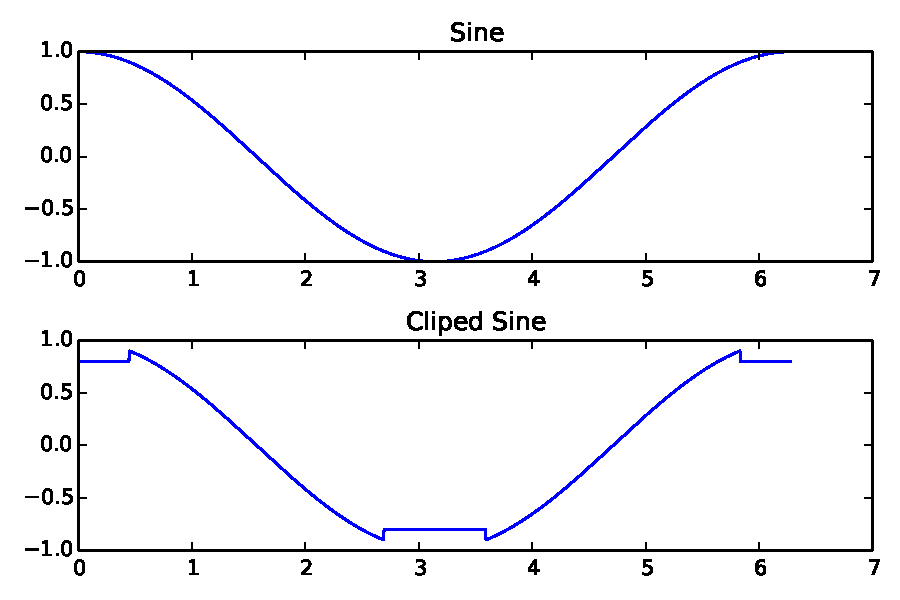
\includegraphics[width=0.8\textwidth]{./pyJvsip_examples/eXclip}\captionof{figure}{Clip Example}
\label{fig:ClipExample}\end{minipage}
\pyComment{
\item{The clip function works much the same as \cvl{} except the output is returned. In line 6 of the example we used the \ttbf{empty} method to create the output vector and saved a reference in the left value.}
\item{The \ttbf{clip} function is a bit complicated. See the \cvl{} specification for more complete details.}
\item{The \ttbf{view} \ttbf{in} is clipped according to the rules of the function. The clipping checks are set by \ttbf{t1} and \ttbf{t2} and the clip values are set by \ttbf{c1} and \ttbf{c2} accordingly. The output is placed in \ttbf{out}. If \ttbf{in==out} then the function is done in-place}
}
\afunc{cmplx}{ \ref{tab:manipulationOperations}.}
\\\cvsiplh
\\\pyjvsiph

\afuncT{conj}{Conjugate each element in a view. An Unary Operations.}{unaryOperations}
\\\cvsiplh
\afh
\\\hspace*{.04\textwidth} {
\ttfamily
\begin{tabular}[H]{l}
vsip\_cscalar\_d vsip\_conj\_d(vsip\_cscalar\_d);\\
vsip\_cscalar\_f vsip\_conj\_f(vsip\_cscalar\_f);\\
void vsip\_cmconj\_d(\\*\hspace*{1cm}const vsip\_cmview\_d*, const vsip\_cmview\_d*);\\
void vsip\_cmconj\_f(\\*\hspace*{1cm}const vsip\_cmview\_f*, const vsip\_cmview\_f*);\\
void vsip\_cvconj\_d(\\*\hspace*{1cm}const vsip\_cvview\_d*, const vsip\_cvview\_d*);\\
void vsip\_cvconj\_f(\\*\hspace*{1cm}const vsip\_cvview\_f*, const vsip\_cvview\_f*);\\
\end{tabular}
}
\\\pyjvsiph
\viewmthd{yes}{yes}{yes}{inOut.conj}
\apyfunc{yes}{out = conj(in,out)}
\pyComment{

\item{The \ttbf{conj} function works much the same as the C VSIPL version except that a convenience pointer to the output view is returned. This may be done in-place if \ttbf{in==out}.}
\item{If the calling \ttbf{view} for the \ttbf{conj} method is real no error is generated. This case is basically a no operation. This is not true for the \ttbf{conj} function call which will generate an assert error as an unsupported type.}
}
\clearpage
{\large \textbf{\hypertarget{convFunc}{CONV Class}}}\vspace{.2cm}\\
\hspace*{.3cm}
\parbox{0.85\textwidth}{Discrete Fourier Transforms. See FFT Functions table \ref{tab:fftFunctions}}
\cvsiplh 
\newline \hspace*{.8cm} \vspace*{.1cm} \textbf{Available Functions }
\newline \hspace*{.8cm} \vspace*{.1cm} \texttt{fft\_create}
\newline \hspace*{1.1cm} {
\ttfamily
\begin{tabular}[H]{l}
vsip\_rcfir\_d* vsip\_rcfir\_create\_d(\\*\hspace{.7cm}const vsip\_vview\_d*, vsip\_symmetry, vsip\_length,\\*\hspace{.7cm}vsip\_length, vsip\_obj\_state, unsigned, vsip\_alg\_hint);\\
\end{tabular}
}
\newline \hspace*{.8cm} \vspace*{.1cm} \texttt{fft\_destroy}
\newline \hspace*{1.1cm} {
\ttfamily
\begin{tabular}[H]{l}
int vsip\_fft\_destroy\_d(vsip\_fft\_d*);\\
\end{tabular}
}\vspace{.1cm}
\newline \hspace*{.8cm} \vspace*{.1cm} \texttt{fft}
\newline \hspace*{1.1cm} {
\ttfamily
\begin{tabular}[H]{l}
int vsip\_rcfirflt\_d(vsip\_rcfir\_d*, const vsip\_cvview\_d*,\\*\hspace{.7cm}const vsip\_cvview\_d*);\\
\end{tabular}
}
\clearpage
\hspace*{.8cm} \texttt{fft\_getattr}
\newline \hspace*{1.1cm} {
\ttfamily
\begin{tabular}[H]{l}
void vsip\_rcfir\_getattr\_d(const vsip\_rcfir\_d*,\\*\hspace{.7cm}vsip\_rcfir\_attr*);\\
\end{tabular}
}\vspace{.1cm}
\newline\hspace*{.8cm} \texttt{fir\_reset}
\newline \hspace*{1.1cm} {
\ttfamily
\begin{tabular}[H]{l}
void vsip\_rcfir\_reset\_d(vsip\_rcfir\_d*)\\
\end{tabular}\
}
\pyjvsiph
\afunc{copy}{Copy Data between two views. Some mixed types are supported so this method can be used to produce a copy of data of a new precision}
\\\cvsiplh
\newline \hspace*{.8cm} \vspace*{.1cm} \textbf{Available Functions }
\newline \hspace*{1cm} {\ttfamily
\begin{tabular}[H]{l}
void vsip\_cmcopy\_d\_d(\\*
\hspace{1cm}const vsip\_cmview\_d*, const vsip\_cmview\_d*);\\
void vsip\_cmcopy\_d\_f(\\*
\hspace{1cm}const vsip\_cmview\_d*, const vsip\_cmview\_f*);\\
void vsip\_cmcopy\_f\_d(\\*
\hspace{1cm}const vsip\_cmview\_f*, const vsip\_cmview\_d*);\\
void vsip\_cmcopy\_f\_f(\\*
\hspace{1cm}const vsip\_cmview\_f*, const vsip\_cmview\_f*);\\
void vsip\_cvcopy\_d\_d\\*
\hspace{1cm}(const vsip\_cvview\_d*, const vsip\_cvview\_d*);\\
$\cdots$  \emph{etc.} \end{tabular}
}
\newline \hspace*{1cm}
\parbox{11cm}{There are many copy functions. To see all supported search the \ilCode{vsip.h} header file.\footnotemark}
\footnotetext{For instance \ttbf{grep copy\_ vsip.h} will list all available copy functions.}
\\\pyjvsiph
\viewmthd{yes}{yes}{no}{\parbox[t]{4cm}{out=in.copy\\out=in.copyrm\\out=in.copycm}}
\newline\hspace*{1cm}\parbox{11cm}{The \ttbf{copy} method creates a new view and data space that is the same shape, precision and depth as the input view and copies the data from the \ilCode{in} view to the \ilCode{out} view. The block in the \ilCode{out} view will be the exact size needed to hold the data and will be unit stride along the major direction of the \ilCode{in} view.\\The {\texttt{\bfseries{copycm}}} method is the same as the \ilCode{copy} method except the output view will always be row major independent of the input views major direction.\\The \ttbf{copyrm} method is the same as the \ilCode{copy} method except the output view will always be column major independent of the input views major direction.\\If the input view is a vector the three copy methods have identical results.}
\newline
\apyfunc{yes}{out = copy(in,out)}
\newline\hspace*{1cm}\parbox{11cm}{The \ttbf{copy} function works much the same as the C VSIPL version except that a convenience pointer to the output view is returned.}

\clearpage
{\large \textbf{\hypertarget{copyfrom}{copyfrom\_user}}\\
{ \ref{tab:elementGenerationOperations}.}
\\\cvsiplh
\\\pyjvsiph

\clearpage
{\large \textbf{\hypertarget{copyto}{copyto\_user}}\\
{ \ref{tab:elementGenerationOperations}.}
\\\cvsiplh
\\\pyjvsiph

\afuncT{corr}{Correlation Function Set.}{convCorrFunctions} 
\\\cvsiplh
\\\pyjvsiph
\afuncT{cos}{Cosine; An elementary math function.}{elementaryMath}
\\\cvsiplh
\afh
\\\hspace*{.04\textwidth} {
\ttfamily
\begin{tabular}[H]{l}
vsip\_scalar\_f vsip\_cos\_f(vsip\_scalar\_f a);\\
vsip\_scalar\_d vsip\_cos\_d(vsip\_scalar\_d a);\\
void vsip\_mcos\_d(const vsip\_mview\_d*, const vsip\_mview\_d*);\\
void vsip\_mcos\_f(const vsip\_mview\_f*, const vsip\_mview\_f*);\\
void vsip\_vcos\_d(const vsip\_vview\_d*, const vsip\_vview\_d*);\\
void vsip\_vcos\_f(const vsip\_vview\_f*, const vsip\_vview\_f*);\\
\end{tabular}
}
\\\pyjvsiph
\viewmthd{yes}{yes}{yes}{inOut.cos}
\apyfunc{yes}{out = cos(in,out)}
\pyComment{
\item{The \ttbf{cos} function works much the same as the C VSIPL version except that a convenience pointer to the output view is returned. This may be done in-place if \ttbf{in==out}.}}

\afuncT{cosh}{Hyperbolic Cosine; An elementwise function}{elementaryMath}
\\\cvsiplh
\afh
\\\hspace*{.04\textwidth} {
\ttfamily
\begin{tabular}[H]{l}
vsip\_scalar\_f vsip\_cosh\_f(vsip\_scalar\_f a);\\
vsip\_scalar\_d vsip\_cosh\_d(vsip\_scalar\_d a);\\
void vsip\_mcosh\_d(const vsip\_mview\_d*, const vsip\_mview\_d*);\\
void vsip\_mcosh\_f(const vsip\_mview\_f*, const vsip\_mview\_f*);\\
void vsip\_vcosh\_d(const vsip\_vview\_d*, const vsip\_vview\_d*);\\
void vsip\_vcosh\_f(const vsip\_vview\_f*, const vsip\_vview\_f*);\\
\end{tabular}
}
\\\pyjvsiph
\viewmthd{yes}{yes}{yes}{inOut.cosh}
\apyfunc{yes}{out = cosh(in,out)}
\pyComment{
\item{The \ttbf{cosh} function works much the same as the C VSIPL version except that a convenience pointer to the output view is returned. This may be done in-place if \ttbf{in==out}.}}

\afunc{covsol}{Solve linear least squares problem. \ref{tab:specialLinearSystemSolvers}.}
\\\cvsiplh
\newline \hspace*{.8cm} \vspace*{.1cm} \textbf{Available Functions }
\newline \hspace*{1.1cm} {
\ttfamily
\begin{tabular}[H]{l}
\end{tabular}
}
\\\pyjvsiph

\afunc{cumsum}{Cumulative Sum}
\index{Cumulative Sum}
\\\cvsiplh
\\\pyjvsiph
\hspace*{1cm}\texttt{
\begin{tabular}[H]{l}
vsip\_block\_bl* vsip\_mdestroy\_bl(vsip\_mview\_bl*);\\
vsip\_block\_bl* vsip\_vdestroy\_bl(vsip\_vview\_bl*);\\
vsip\_block\_d* vsip\_tdestroy\_d(vsip\_tview\_d*);\\
vsip\_block\_d* vsip\_mdestroy\_d(vsip\_mview\_d*);\\
vsip\_block\_d* vsip\_vdestroy\_d(vsip\_vview\_d*);\\
vsip\_block\_f* vsip\_tdestroy\_f(vsip\_tview\_f*);\\
vsip\_block\_f* vsip\_mdestroy\_f(vsip\_mview\_f*);\\
vsip\_block\_f* vsip\_vdestroy\_f(vsip\_vview\_f*);\\
vsip\_block\_i* vsip\_tdestroy\_i(vsip\_tview\_i*);\\
vsip\_block\_i* vsip\_mdestroy\_i(vsip\_mview\_i*);\\
vsip\_block\_i* vsip\_vdestroy\_i(vsip\_vview\_i*);\\
vsip\_block\_mi* vsip\_vdestroy\_mi(vsip\_vview\_mi*);\\
vsip\_block\_si* vsip\_tdestroy\_si(vsip\_tview\_si*);\\
vsip\_block\_si* vsip\_mdestroy\_si(vsip\_mview\_si*);\\
vsip\_block\_si* vsip\_vdestroy\_si(vsip\_vview\_si*);\\
vsip\_block\_uc* vsip\_tdestroy\_uc(vsip\_tview\_uc*);\\
vsip\_block\_uc* vsip\_mdestroy\_uc(vsip\_mview\_uc*);\\
vsip\_block\_uc* vsip\_vdestroy\_uc(vsip\_vview\_uc*);\\
vsip\_block\_vi* vsip\_vdestroy\_vi(vsip\_vview\_vi*);\\
vsip\_cblock\_d* vsip\_ctdestroy\_d(vsip\_ctview\_d*);\\
vsip\_cblock\_d* vsip\_cmdestroy\_d(vsip\_cmview\_d*);\\
vsip\_cblock\_d* vsip\_cvdestroy\_d(vsip\_cvview\_d*);\\
vsip\_cblock\_f* vsip\_ctdestroy\_f(vsip\_ctview\_f*);\\
vsip\_cblock\_f* vsip\_cmdestroy\_f(vsip\_cmview\_f*);\\
vsip\_cblock\_f* vsip\_cvdestroy\_f(vsip\_cvview\_f*);\\
\end{tabular}
}
\newline\hspace*{1cm}\texttt{
\begin{tabular}[H]{l}
int vsip\_chold\_destroy\_d(vsip\_chol\_d*);\\
int vsip\_chold\_destroy\_f(vsip\_chol\_f*);\\
int vsip\_cchold\_destroy\_d(vsip\_cchol\_d*);\\
int vsip\_cchold\_destroy\_f(vsip\_cchol\_f*);\\
\end{tabular}
}
\newline\hspace*{1cm}\texttt{
\begin{tabular}[H]{l}
int vsip\_corr1d\_destroy\_d(vsip\_corr1d\_d*);\\
int vsip\_corr1d\_destroy\_f(vsip\_corr1d\_f*);\\
int vsip\_ccorr1d\_destroy\_d(vsip\_ccorr1d\_d*);\\
int vsip\_ccorr1d\_destroy\_f(vsip\_ccorr1d\_f *cor);\\
\end{tabular}
}
\newline\hspace*{1cm}\texttt{
\begin{tabular}[H]{l}
int vsip\_fir\_destroy\_d(vsip\_fir\_d*);\\
int vsip\_fir\_destroy\_f(vsip\_fir\_f*);\\
int vsip\_rcfir\_destroy\_d(vsip\_rcfir\_d*);\\
int vsip\_rcfir\_destroy\_f(vsip\_rcfir\_f*);\\
int vsip\_cfir\_destroy\_d(vsip\_cfir\_d*);\\
int vsip\_cfir\_destroy\_f(vsip\_cfir\_f*);\\
\end{tabular}
}
\newline\hspace*{1cm}\texttt{
\begin{tabular}[H]{l}
\end{tabular}
}
\newline\hspace*{1cm}\texttt{
\begin{tabular}[H]{l}
int vsip\_lud\_destroy\_d(vsip\_lu\_d*);\\
int vsip\_lud\_destroy\_f(vsip\_lu\_f*);\\
int vsip\_clud\_destroy\_d(vsip\_clu\_d*);\\
int vsip\_clud\_destroy\_f(vsip\_clu\_f*);\\
\end{tabular}
}
\newline\hspace*{1cm}\texttt{
\begin{tabular}[H]{l}
int vsip\_conv1d\_destroy\_d(vsip\_conv1d\_d*);\\
int vsip\_conv1d\_destroy\_f(vsip\_conv1d\_f*);\\
\end{tabular}
}
\newline\hspace*{1cm}\texttt{
\begin{tabular}[H]{l}
int vsip\_qrd\_destroy\_d(vsip\_qr\_d*);\\
int vsip\_qrd\_destroy\_f(vsip\_qr\_f*);\\
int vsip\_cqrd\_destroy\_d(vsip\_cqr\_d*);\\
int vsip\_cqrd\_destroy\_f(vsip\_cqr\_f*);\\
\end{tabular}
}
\newline\hspace*{1cm}\texttt{
\begin{tabular}[H]{l}
int vsip\_fft\_destroy\_d(vsip\_fft\_d*);\\
int vsip\_fft\_destroy\_f(vsip\_fft\_f*);\\
\end{tabular}
}
\newline\hspace*{1cm}\texttt{
\begin{tabular}[H]{l}
int vsip\_fftm\_destroy\_d(vsip\_fftm\_d*);\\
int vsip\_fftm\_destroy\_f(vsip\_fftm\_f*);\\
\end{tabular}
}
\newline\hspace*{1cm}\texttt{
\begin{tabular}[H]{l}
int vsip\_randdestroy(vsip\_randstate *) ;\\
\end{tabular}
}
\newline\hspace*{1cm}\texttt{
\begin{tabular}[H]{l}
void vsip\_blockdestroy\_bl(vsip\_block\_bl*);\\
void vsip\_blockdestroy\_d(vsip\_block\_d*);\\
void vsip\_blockdestroy\_f(vsip\_block\_f*);\\
void vsip\_blockdestroy\_i(vsip\_block\_i*);\\
void vsip\_blockdestroy\_mi(vsip\_block\_mi*);\\
void vsip\_blockdestroy\_si(vsip\_block\_si*);\\
void vsip\_blockdestroy\_uc(vsip\_block\_uc*);\\
void vsip\_blockdestroy\_vi(vsip\_block\_vi *);\\
void vsip\_cblockdestroy\_d(vsip\_cblock\_d*);\\
void vsip\_cblockdestroy\_f(vsip\_cblock\_f*);\\
\end{tabular}
}
\newline\hspace*{1cm}\texttt{
\begin{tabular}[H]{l}
void vsip\_cmalldestroy\_d(vsip\_cmview\_d*);\\
void vsip\_cmalldestroy\_f(vsip\_cmview\_f*);\\
void vsip\_ctalldestroy\_d(vsip\_ctview\_d*);\\
void vsip\_ctalldestroy\_f(vsip\_ctview\_f*);\\
void vsip\_cvalldestroy\_d(vsip\_cvview\_d*);\\
void vsip\_cvalldestroy\_f(vsip\_cvview\_f*);\\
void vsip\_malldestroy\_bl(vsip\_mview\_bl*);\\
void vsip\_malldestroy\_d(vsip\_mview\_d*);\\
void vsip\_malldestroy\_f(vsip\_mview\_f*);\\
void vsip\_malldestroy\_i(vsip\_mview\_i*);\\
void vsip\_malldestroy\_si(vsip\_mview\_si*);\\
void vsip\_malldestroy\_uc(vsip\_mview\_uc*);\\
void vsip\_talldestroy\_d(vsip\_tview\_d*);\\
void vsip\_talldestroy\_f(vsip\_tview\_f*);\\
void vsip\_talldestroy\_i(vsip\_tview\_i*);\\
void vsip\_talldestroy\_si(vsip\_tview\_si*);\\
void vsip\_talldestroy\_uc(vsip\_tview\_uc*);\\
void vsip\_valldestroy\_bl(vsip\_vview\_bl*);\\
void vsip\_valldestroy\_d(vsip\_vview\_d*);\\
void vsip\_valldestroy\_f(vsip\_vview\_f*);\\
void vsip\_valldestroy\_i(vsip\_vview\_i*);\\
void vsip\_valldestroy\_mi(vsip\_vview\_mi*);\\
void vsip\_valldestroy\_si(vsip\_vview\_si*);\\
void vsip\_valldestroy\_uc(vsip\_vview\_uc*);\\
void vsip\_valldestroy\_vi(vsip\_vview\_vi*);\\
\end{tabular}
}
\newline\hspace*{1cm}\texttt{
\begin{tabular}[H]{l}
void vsip\_permute\_destroy(vsip\_permute*);\\
\end{tabular}
}
\newline\hspace*{1cm}\texttt{
\begin{tabular}[H]{l}
void vsip\_spline\_destroy\_d(vsip\_spline\_d *);\\
void vsip\_spline\_destroy\_f(vsip\_spline\_f *);\\
\end{tabular}
}
\newline\hspace*{1cm}\texttt{
\begin{tabular}[H]{l}
int vsip\_svd\_destroy\_f(vsip\_sv\_f* );\\
int vsip\_csvd\_destroy\_f(vsip\_csv\_f* svd);\\
int vsip\_svd\_destroy\_d(vsip\_sv\_d* );\\
int vsip\_csvd\_destroy\_d(vsip\_csv\_d* svd);\\
\end{tabular}
}

\afuncT{div}{Divide two \ttbf{view}s, a scalar and a \ttbf{view} or a \ttbf{view} and a scalar. A binary operation.}{binaryOperations}
\\\cvsiplh
\\
\hspace*{.04\textwidth}\parbox{.93\textwidth}{
\textrm{There are many combinations of divide available in \jv{}. The specification provides the normal \ttbf{view} divides of complex-complex and real-real types;\Bs but also provides real-complex and complex-real divides as well as mixed \ttbf{scalar-view} and \ttbf{view-scalar} divides. Consequently the listed available functions are broken up into several tables below.}
}\vspace{2mm}
\\
\afh
{
\ttfamily
\\\hspace*{.04\textwidth}\begin{tabular}[H]{l}
\multicolumn{1}{c}{\Ts\rmfamily \bfseries Scalar Functions}\\ \hline
vsip\_cscalar\_d vsip\_cdiv\_d(vsip\_cscalar\_d, vsip\_cscalar\_d);\Bs\\
vsip\_cscalar\_d vsip\_crdiv\_d(vsip\_cscalar\_d, vsip\_scalar\_d);\Bs\\
vsip\_cscalar\_f vsip\_cdiv\_f(vsip\_cscalar\_f, vsip\_cscalar\_f);\Bs\\
vsip\_cscalar\_f vsip\_crdiv\_f(vsip\_cscalar\_f, vsip\_scalar\_f);\Bs\\
\end{tabular}\\
\hspace*{.04\textwidth}\begin{tabular}[H]{l}
\multicolumn{1}{c}{\Ts\rmfamily \bfseries Normal View Functions}\\ \hline
void vsip\_vdiv\_d(\\*\hspace*{1cm}const vsip\_vview\_d*, const vsip\_vview\_d*,const vsip\_vview\_d*);\Bs\\
void vsip\_vdiv\_f(\\*\hspace*{1cm}const vsip\_vview\_f*, const vsip\_vview\_f*,const vsip\_vview\_f*);\Bs\\
void vsip\_mdiv\_d(\\*\hspace*{1cm}const vsip\_mview\_d*, const vsip\_mview\_d*,const vsip\_mview\_d*);\Bs\\
void vsip\_mdiv\_f(\\*\hspace*{1cm}const vsip\_mview\_f*, const vsip\_mview\_f*,const vsip\_mview\_f*);\Bs\\
void vsip\_cvdiv\_d(\\*\hspace*{1cm}const vsip\_cvview\_d*, const vsip\_cvview\_d*,const vsip\_cvview\_d*);\Bs\\
void vsip\_cvdiv\_f(\\*\hspace*{1cm}const vsip\_cvview\_f*, const vsip\_cvview\_f*,const vsip\_cvview\_f*);\Bs\\
void vsip\_cmdiv\_d(\\*\hspace*{1cm}const vsip\_cmview\_d*, const vsip\_cmview\_d*,const vsip\_cmview\_d*);\Bs\\
void vsip\_cmdiv\_f(\\*\hspace*{1cm}const vsip\_cmview\_f*, const vsip\_cmview\_f*,const vsip\_cmview\_f*);\Bs\\
\end{tabular}\\
\hspace*{.04\textwidth}\begin{tabular}[H]{l}
\multicolumn{1}{c}{\Ts\rmfamily \bfseries Mixed Depth View Functions}\\ \hline
void vsip\_rcvdiv\_d(\\*\hspace*{1cm}const vsip\_vview\_d*, const vsip\_cvview\_d*,const vsip\_cvview\_d*);\Bs\\
void vsip\_rcvdiv\_f(\\*\hspace*{1cm}const vsip\_vview\_f*, const vsip\_cvview\_f*,const vsip\_cvview\_f*);\Bs\\
void vsip\_crvdiv\_d(\\*\hspace*{1cm}const vsip\_cvview\_d*, const vsip\_vview\_d*,const vsip\_cvview\_d*);\Bs\\
void vsip\_crvdiv\_f(\\*\hspace*{1cm}const vsip\_cvview\_f*, const vsip\_vview\_f*,const vsip\_cvview\_f*);\Bs\\
void vsip\_rcmdiv\_d(\\*\hspace*{1cm}const vsip\_mview\_d*, const vsip\_cmview\_d*,const vsip\_cmview\_d*);\Bs\\
void vsip\_rcmdiv\_f(\\*\hspace*{1cm}const vsip\_mview\_f*, const vsip\_cmview\_f*,const vsip\_cmview\_f*);\Bs\\
void vsip\_crmdiv\_d(\\*\hspace*{1cm}const vsip\_cmview\_d*, const vsip\_mview\_d*,const vsip\_cmview\_d*);\Bs\\
void vsip\_crmdiv\_f(\\*\hspace*{1cm}const vsip\_cmview\_f*, const vsip\_mview\_f*,const vsip\_cmview\_f*);\Bs\\
\end{tabular}\\
\hspace*{.04\textwidth}\begin{tabular}[H]{l}
\multicolumn{1}{c}{\Ts\rmfamily \bfseries View Divide Scalar Functions}\\ \hline
void vsip\_vsdiv\_d(\\*\hspace*{1cm}const vsip\_vview\_d*, vsip\_scalar\_d,const vsip\_vview\_d*);\Bs\\
void vsip\_vsdiv\_f(\\*\hspace*{1cm}const vsip\_vview\_f*, vsip\_scalar\_f,const vsip\_vview\_f*);\Bs\\
void vsip\_cvrsdiv\_d(\\*\hspace*{1cm}const vsip\_cvview\_d*, vsip\_scalar\_d,const vsip\_cvview\_d*);\Bs\\
void vsip\_cvrsdiv\_f(\\*\hspace*{1cm}const vsip\_cvview\_f*, vsip\_scalar\_f,const vsip\_cvview\_f*);\Bs\\
void vsip\_msdiv\_d(\\*\hspace*{1cm}const vsip\_mview\_d*, vsip\_scalar\_d,const vsip\_mview\_d*);\Bs\\
void vsip\_msdiv\_f(\\*\hspace*{1cm}const vsip\_mview\_f*, vsip\_scalar\_f,const vsip\_mview\_f*);\Bs\\
void vsip\_cmrsdiv\_d(\\*\hspace*{1cm}const vsip\_cmview\_d*, vsip\_scalar\_d,const vsip\_cmview\_d*);\Bs\\
void vsip\_cmrsdiv\_f(\\*\hspace*{1cm}const vsip\_cmview\_f*, vsip\_scalar\_f,const vsip\_cmview\_f*);\Bs\\
\end{tabular}\\
\hspace*{.04\textwidth}\begin{tabular}[H]{l}
\multicolumn{1}{c}{\Ts\rmfamily \bfseries Scalar Divide View Functions}\\ \hline
void vsip\_svdiv\_d(\\*\hspace*{1cm}vsip\_scalar\_d, const vsip\_vview\_d*,const vsip\_vview\_d*);\Bs\\
void vsip\_svdiv\_f(\\*\hspace*{1cm}vsip\_scalar\_f, const vsip\_vview\_f*,const vsip\_vview\_f*);\Bs\\
void vsip\_rscvdiv\_d(\\*\hspace*{1cm}vsip\_scalar\_d, const vsip\_cvview\_d*,const vsip\_cvview\_d*);\Bs\\
void vsip\_rscvdiv\_f(\\*\hspace*{1cm}vsip\_scalar\_f, const vsip\_cvview\_f*,const vsip\_cvview\_f*);\Bs\\
void vsip\_csvdiv\_d(\\*\hspace*{1cm}vsip\_cscalar\_d, const vsip\_cvview\_d*,const vsip\_cvview\_d*);\Bs\\
void vsip\_csvdiv\_f(\\*\hspace*{1cm}vsip\_cscalar\_f, const vsip\_cvview\_f*,const vsip\_cvview\_f*);\Bs\\
void vsip\_smdiv\_d(\\*\hspace*{1cm}vsip\_scalar\_d, const vsip\_mview\_d*,const vsip\_mview\_d*);\Bs\\
void vsip\_smdiv\_f(\\*\hspace*{1cm}vsip\_scalar\_f, const vsip\_mview\_f*,const vsip\_mview\_f*);\Bs\\
void vsip\_rscmdiv\_d(\\*\hspace*{1cm}vsip\_scalar\_d, const vsip\_cmview\_d*,const vsip\_cmview\_d*);\Bs\\
void vsip\_rscmdiv\_f(\\*\hspace*{1cm}vsip\_scalar\_f, const vsip\_cmview\_f*,const vsip\_cmview\_f*);\Bs\\
void vsip\_csmdiv\_d(\\*\hspace*{1cm}vsip\_cscalar\_d, const vsip\_cmview\_d*,const vsip\_cmview\_d*);\Bs\\
void vsip\_csmdiv\_f(\\*\hspace*{1cm}vsip\_cscalar\_f, const vsip\_cmview\_f*,const vsip\_cmview\_f*);\Bs\\
\end{tabular}\\
}
\\\pyjvsiph
\\\vmthdh
\hspace*{.06\textwidth}Overloaded on divide operator.\\
\hspace*{.06\textwidth}\textbf{In Place: }\hspace{.2cm} yes\\
\hspace*{.08\textwidth}\textbf{Example: }\ttbf{a /= b; a /= 2}\\*
\hspace*{.1\textwidth}Elements of \ttbf{view a} replaced with result.\\
\hspace*{.06\textwidth}\textbf{Out of Place: }\hspace{.2cm} yes\\
\hspace*{.08\textwidth}\textbf{Example: }\ttbf{c = a / b; d = 2 / c; e = c / 2}\\*
\hspace*{.1\textwidth}\parbox{.85\textwidth}{\ttbf{view c}, \ttbf{view d}, and \ttbf{view e}  created and filled with result of operation.}\\
\\\hspace*{.04\textwidth}{\textbf{Function}\vspace{.2cm}}\\
\hspace*{.06\textwidth}\parbox{.93\textwidth}{The divide function works the same as C VSIPL except a convenience copy of the output view will return.\vspace{.2cm}}\\
\hspace*{.08\textwidth}\textbf{Example: }\ttbf{c = div(a,b,c)}\\
\hspace*{.1\textwidth}Variables \ttbf{a} and \ttbf{b} are both \ttbf{view}s or \ttbf{a} OR \ttbf{b} may be a scalar.\\
\hspace*{.1\textwidth}Variable \ttbf{c} is a compliant output \ttbf{view}.\\
\hspace*{.1\textwidth}In place means \ttbf{c} is the same as \ttbf{a} or \ttbf{b}.\\
\hspace*{.1\textwidth}The function will complain if input variable combination is not supported.\\


\afuncT{dot}{Vector Dot Product }{matrixOperations}
\\\cvsiplh
\\ \hspace*{.8cm} \vspace*{.1cm} \textbf{Available Functions }
\\ \hspace*{1.1cm} {
\ttfamily
\begin{tabular}[H]{l}
vsip\_cscalar\_d vsip\_cvdot\_d(\\*\hspace{.6cm}const vsip\_cvview\_d*, const vsip\_cvview\_d*);\\
vsip\_cscalar\_f vsip\_cvdot\_f(\\*\hspace{.6cm}const vsip\_cvview\_f*, const vsip\_cvview\_f*);\\
vsip\_scalar\_d vsip\_vdot\_d(\\*\hspace{.6cm}const vsip\_vview\_d*, const vsip\_vview\_d*);\\
vsip\_scalar\_f vsip\_vdot\_f(\\*\hspace{.6cm}const vsip\_vview\_f*, const vsip\_vview\_f*);\\
\end{tabular}
}
\\\pyjvsiph

\afunc{euler}{Euler}
\\\cvsiplh
\\\pyjvsiph
\afuncT{exp10}{exp10onential Base 10; An elementwise function}{elementaryMath}
\\\cvsiplh
\\ \hspace*{.8cm} \vspace*{.1cm} \textbf{Available Functions }
\\ \hspace*{1.1cm} {
\ttfamily
\begin{tabular}[H]{l}
vsip\_scalar\_d vsip\_exp10\_d(vsip\_scalar\_d);\\
vsip\_scalar\_f vsip\_exp10\_f(vsip\_scalar\_f);\\
void vsip\_mexp10\_d(const vsip\_mview\_d*, const vsip\_mview\_d*);\\
void vsip\_mexp10\_f(const vsip\_mview\_f*, const vsip\_mview\_f*);\\
void vsip\_vexp10\_d(const vsip\_vview\_d*, const vsip\_vview\_d*);\\
void vsip\_vexp10\_f(const vsip\_vview\_f*, const vsip\_vview\_f*);\\
\end{tabular}
}
\\\pyjvsiph
\viewmthd{yes}{yes}{yes}{inOut.exp10}
\apyfunc{yes}{out = exp10(in,out)}
\pyComment{\item{The \ttbf{exp10} function works much the same as the C VSIPL version except that a convenience pointer to the output view is returned. This may be done in-place if \ttbf{in==out}.}}

\afuncT{exp}{Exponential; An elementwise function}{elementaryMath}
\\\cvsiplh
\afh
\\\hspace*{.04\textwidth} {
\ttfamily
\begin{tabular}[H]{l}
vsip\_cscalar\_d vsip\_cexp\_d(vsip\_cscalar\_d);\\
vsip\_cscalar\_f vsip\_cexp\_f(vsip\_cscalar\_f);\\
void vsip\_cmexp\_d(const vsip\_cmview\_d*, const vsip\_cmview\_d*);\\
void vsip\_cmexp\_f(const vsip\_cmview\_f*, const vsip\_cmview\_f*);\\
void vsip\_cvexp\_d(const vsip\_cvview\_d*, const vsip\_cvview\_d*);\\
void vsip\_cvexp\_f(const vsip\_cvview\_f*, const vsip\_cvview\_f*);\\
void vsip\_mexp\_d(const vsip\_mview\_d*, const vsip\_mview\_d*);\\
void vsip\_mexp\_f(const vsip\_mview\_f*, const vsip\_mview\_f*);\\
void vsip\_vexp\_d(const vsip\_vview\_d*, const vsip\_vview\_d*);\\
void vsip\_vexp\_f(const vsip\_vview\_f*, const vsip\_vview\_f*);\\
\end{tabular}
}
\\\pyjvsiph
\viewmthd{yes}{yes}{yes}{inOut.exp}
\apyfunc{yes}{out = exp(in,out)}
\pyComment{\item{The \ttbf{exp} function works much the same as the C VSIPL version except that a convenience pointer to the output view is returned. This may be done in-place if \ttbf{in==out}.}}

\afunc{expoavg}{computes the difference of a scalar and a \ttbf{view} or between two \ttbf{view}s. A binary operation. See table \ref{tab:binaryOperations}.}
\\\cvsiplh
\\\pyjvsiph
\clearpage
{\large \textbf{\hypertarget{fftFunc}{FFT Class}}}\vspace{.2cm}\\
\hspace*{.3cm}
\parbox{0.85\textwidth}{Discrete Fourier Transforms. See FFT Functions table \ref{tab:fftFunctions}}
\cvsiplh 
\newline \hspace*{.8cm} \vspace*{.1cm} \textbf{Available Functions }
\newline \hspace*{.8cm} \vspace*{.1cm} \texttt{fft\_create}
\newline \hspace*{1.1cm} {
\ttfamily
\begin{tabular}[H]{l}
vsip\_rcfir\_d* vsip\_rcfir\_create\_d(\\*\hspace{.7cm}const vsip\_vview\_d*, vsip\_symmetry, vsip\_length,\\*\hspace{.7cm}vsip\_length, vsip\_obj\_state, unsigned, vsip\_alg\_hint);\\
\end{tabular}
}
\newline \hspace*{.8cm} \vspace*{.1cm} \texttt{fft\_destroy}
\newline \hspace*{1.1cm} {
\ttfamily
\begin{tabular}[H]{l}
int vsip\_fft\_destroy\_d(vsip\_fft\_d*);\\
\end{tabular}
}\vspace{.1cm}
\newline \hspace*{.8cm} \vspace*{.1cm} \texttt{fft}
\newline \hspace*{1.1cm} {
\ttfamily
\begin{tabular}[H]{l}
int vsip\_rcfirflt\_d(vsip\_rcfir\_d*, const vsip\_cvview\_d*,\\*\hspace{.7cm}const vsip\_cvview\_d*);\\
\end{tabular}
}
\clearpage
\hspace*{.8cm} \texttt{fft\_getattr}
\newline \hspace*{1.1cm} {
\ttfamily
\begin{tabular}[H]{l}
void vsip\_rcfir\_getattr\_d(const vsip\_rcfir\_d*,\\*\hspace{.7cm}vsip\_rcfir\_attr*);\\
\end{tabular}
}\vspace{.1cm}
\newline\hspace*{.8cm} \texttt{fir\_reset}
\newline \hspace*{1.1cm} {
\ttfamily
\begin{tabular}[H]{l}
void vsip\_rcfir\_reset\_d(vsip\_rcfir\_d*)\\
\end{tabular}\
}
\pyjvsiph
\afuncT{fill}{Fill a \ttbf{view} with a value.}{elementGenerationOperations}
\\\cvsiplh
\\ \hspace*{.8cm} \vspace*{.1cm} \textbf{Available Functions }
\\ \hspace*{1cm} {\ttfamily
\begin{tabular}[H]{l}
void vsip\_cmfill\_d(vsip\_cscalar\_d, const vsip\_cmview\_d*);\\
void vsip\_cmfill\_f(vsip\_cscalar\_f, const vsip\_cmview\_f*);\\
void vsip\_cvfill\_d(vsip\_cscalar\_d, const vsip\_cvview\_d*);\\
void vsip\_cvfill\_f(vsip\_cscalar\_f, const vsip\_cvview\_f*);\\
void vsip\_mfill\_d(vsip\_scalar\_d, const vsip\_mview\_d*);\\
void vsip\_mfill\_f(vsip\_scalar\_f, const vsip\_mview\_f*);\\
void vsip\_mfill\_i(vsip\_scalar\_i, const vsip\_mview\_i*);\\
void vsip\_mfill\_si(vsip\_scalar\_si, const vsip\_mview\_si*);\\
void vsip\_mfill\_uc(vsip\_scalar\_uc, const vsip\_mview\_uc*);\\
void vsip\_vfill\_d(vsip\_scalar\_d, const vsip\_vview\_d*);\\
void vsip\_vfill\_f(vsip\_scalar\_f, const vsip\_vview\_f*);\\
void vsip\_vfill\_i(vsip\_scalar\_i, const vsip\_vview\_i*);\\
void vsip\_vfill\_si(vsip\_scalar\_si, const vsip\_vview\_si*);\\
void vsip\_vfill\_uc(vsip\_scalar\_uc, const vsip\_vview\_uc*);\\
void vsip\_vfill\_vi(vsip\_scalar\_vi, const vsip\_vview\_vi*);\\
\end{tabular}}
\\\pyjvsiph
%
\viewmthd{Yes}{No}{Yes}{aView.fill(aScalarValue)}
%
\apyfunc{No}{NA}
%
\pyComment{
\item{Using slicing operator overloaded on equal.}
\subitem {\ttbf{For instance:} \ilCode{aView[:]=aScalarValue} or \ilCode{aView[3:4:3]=aScalarValue}.}
\subitem \ttbf{Caution:} \ilCode{aView=aScalarValue} will turn \ilCode{aView} into \ilCode{aScalarValue} releasing the \ttbf{View}.}
}

\afuncT{finalize}{Finalize \cvl{} before exiting the program. This is hidden (not necessary) in \pyjv{}.}{initSupport}
\\\cvsiplh
\\\pyjvsiph

\clearpage
{\large \textbf{\hypertarget{firFunc}{FIR Class}}}\vspace{.2cm}\\
\hspace*{.3cm}
\parbox{0.85\textwidth}{Finite Impulse Response Class. See filter functions table \ref{tab:filterFunctions}}
\cvsiplh 
\newline \hspace*{.8cm} \vspace*{.1cm} \textbf{Available Functions }
\newline \hspace*{.8cm} \vspace*{.1cm} \texttt{fir\_create}
\newline \hspace*{1.1cm} {
\ttfamily
\begin{tabular}[H]{l}
vsip\_rcfir\_d* vsip\_rcfir\_create\_d(\\*\hspace{.7cm}const vsip\_vview\_d*, vsip\_symmetry, vsip\_length,\\*\hspace{.7cm}vsip\_length, vsip\_obj\_state, unsigned, vsip\_alg\_hint);\\
vsip\_rcfir\_f* vsip\_rcfir\_create\_f(\\*\hspace{.7cm}const vsip\_vview\_f*, vsip\_symmetry, vsip\_length,\\*\hspace{.7cm}vsip\_length, vsip\_obj\_state, unsigned, vsip\_alg\_hint);\\
vsip\_cfir\_d* vsip\_cfir\_create\_d(\\*\hspace{.7cm}const vsip\_cvview\_d*, vsip\_symmetry, vsip\_length,\\*\hspace{.7cm}vsip\_length, vsip\_obj\_state, unsigned, vsip\_alg\_hint);\\
vsip\_cfir\_f* vsip\_cfir\_create\_f(\\*\hspace{.7cm}const vsip\_cvview\_f*, vsip\_symmetry, vsip\_length,\\*\hspace{.7cm}vsip\_length, vsip\_obj\_state, unsigned, vsip\_alg\_hint);\\
vsip\_fir\_d* vsip\_fir\_create\_d(\\*\hspace{.7cm}const vsip\_vview\_d*, vsip\_symmetry, vsip\_length,\\*\hspace{.7cm}vsip\_length, vsip\_obj\_state, unsigned, vsip\_alg\_hint);\\
vsip\_fir\_f* vsip\_fir\_create\_f(\\*\hspace{.7cm}const vsip\_vview\_f*, vsip\_symmetry, vsip\_length,\\*\hspace{.7cm}vsip\_length, vsip\_obj\_state, unsigned, vsip\_alg\_hint);\\
\end{tabular}
}
\newline \hspace*{.8cm} \vspace*{.1cm} \texttt{fir\_destroy}
\newline \hspace*{1.1cm} {
\ttfamily
\begin{tabular}[H]{l}
int vsip\_rcfir\_destroy\_d(vsip\_rcfir\_d*);\\
int vsip\_rcfir\_destroy\_f(vsip\_rcfir\_f*);\\
int vsip\_cfir\_destroy\_d(vsip\_cfir\_d*);\\
int vsip\_cfir\_destroy\_f(vsip\_cfir\_f*);\\
int vsip\_fir\_destroy\_d(vsip\_fir\_d*);\\
int vsip\_fir\_destroy\_f(vsip\_fir\_f*);\\
\end{tabular}
}\vspace{.1cm}
\newline \hspace*{.8cm} \vspace*{.1cm} \texttt{firflt}
\newline \hspace*{1.1cm} {
\ttfamily
\begin{tabular}[H]{l}
int vsip\_rcfirflt\_d(vsip\_rcfir\_d*, const vsip\_cvview\_d*,\\*\hspace{.7cm}const vsip\_cvview\_d*);\\
int vsip\_rcfirflt\_f(vsip\_rcfir\_f*, const vsip\_cvview\_f*,\\*\hspace{.7cm}const vsip\_cvview\_f*);\\
int vsip\_cfirflt\_d(vsip\_cfir\_d*, const vsip\_cvview\_d*,\\*\hspace{.7cm}const vsip\_cvview\_d*);\\
int vsip\_cfirflt\_f(vsip\_cfir\_f*, const vsip\_cvview\_f*,\\*\hspace{.7cm}const vsip\_cvview\_f*);\\
int vsip\_firflt\_d(vsip\_fir\_d*, const vsip\_vview\_d*,\\*\hspace{.7cm}const vsip\_vview\_d*);\\
int vsip\_firflt\_f(vsip\_fir\_f*, const vsip\_vview\_f*,\\*\hspace{.7cm}const vsip\_vview\_f*);\\
\end{tabular}
}
\clearpage
\hspace*{.8cm} \texttt{fir\_getattr}
\newline \hspace*{1.1cm} {
\ttfamily
\begin{tabular}[H]{l}
void vsip\_rcfir\_getattr\_d(const vsip\_rcfir\_d*,\\*\hspace{.7cm}vsip\_rcfir\_attr*);\\
void vsip\_rcfir\_getattr\_f(const vsip\_rcfir\_f*,\\*\hspace{.7cm}vsip\_rcfir\_attr*);\\
void vsip\_cfir\_getattr\_d(const vsip\_cfir\_d*,\\*\hspace{.7cm}vsip\_cfir\_attr*);\\
void vsip\_cfir\_getattr\_f(const vsip\_cfir\_f*,\\*\hspace{.7cm}vsip\_cfir\_attr*);\\
void vsip\_fir\_getattr\_d(const vsip\_fir\_d*,\\*\hspace{.7cm}vsip\_fir\_attr*);\\
void vsip\_fir\_getattr\_f(const vsip\_fir\_f*,\\*\hspace{.7cm}vsip\_fir\_attr*);\\
\end{tabular}
}\vspace{.1cm}
\newline\hspace*{.8cm} \texttt{fir\_reset}
\newline \hspace*{1.1cm} {
\ttfamily
\begin{tabular}[H]{l}
void vsip\_rcfir\_reset\_d(vsip\_rcfir\_d*)\\
void vsip\_rcfir\_reset\_f(vsip\_rcfir\_f*)\\
void vsip\_cfir\_reset\_d(vsip\_cfir\_d*)\\
void vsip\_cfir\_reset\_f(vsip\_cfir\_f*)\\
void vsip\_fir\_reset\_d(vsip\_fir\_d*)\\
void vsip\_fir\_reset\_f(vsip\_fir\_f*)\\
\end{tabular}\
}
\pyjvsiph
\newline\hspace*{.8cm}{\textbf{View Methods\vspace{.2cm}}\\
\hspace*{1cm}\parbox{10.5cm}{
\begin{itemize}
\item {A \ttbf{view} method has been defined.} 
\item {The kernel \ttbf{view} is used as the calling view. The kernel is treated as non-symetric so the entire kernel must be used.}
\item {A variable argument list is supported. The first argument is the input data \ttbf{view} which is required}
\item {The second argument is an integer >= 1 indicating the decimation factor. If the decimation is one then the argument may be left off}
\item{Save state is 'NO' and hints are set to there default values.\vspace{.2cm}}
\end{itemize}}\\
\clearpage
\hspace*{.8cm}{\textbf{FIR Class\vspace{.2cm}}\\
\hspace*{1.cm}\parbox{.9\textwidth}{To create an FIR object use \\*
\hspace*{1.cm} \ttbf{firObj=FIR(t,*args)}\\*
where \ttbf{args} is a tuple containing the create parameters for the FIR type selected, and \ttbf{t} is a string indicating the type of FIR to create.\vspace{.2cm}}\\
\hspace*{1.cm}\parbox{.9\textwidth}{Note \ttbf{args} will contain some or all of the following in the order listed. Each type string is shown in the Finite Impulse Response Filter Types table below.\\
\begin{tabular}[t]{|l l|}\hline
\ttbf{filt} & \parbox[t]{.75\textwidth}{A vector \ttbf{view} of filter coefficients.\\*Required argument \vspace*{.1cm}}\\ \hline
\ttbf{sym} & \parbox[t]{.75\textwidth}{Symmetry of \ttbf{filt} kernel. \\* Required argument\vspace*{.1cm}} \\\hline
\ttbf{N} & \parbox[t]{.75\textwidth}{Length of input data vector. \\* Required argument\vspace*{.1cm}}\\\hline
\ttbf{D} & \parbox[t]{.75\textwidth}{Decimation factor.\\* Required argument\vspace*{.1cm}}\\\hline
\ttbf{state} & \parbox[t]{.75\textwidth}{Flag to indicate if the filter state is to be saved.\\*
VSIP\_STATE\_SAVE or VSIP\_STATE\_NO\_SAVE\\* Argument is supported but defaults to not saving. \\* Instead of \ttbf{VSIP} flags you may use the strings \ttbf{'YES'} or \ttbf{'NO'}.\vspace*{.1cm}}\\ \hline
\ttbf{ntimes} & \parbox[t]{.75\textwidth}{Hint for how much the FIR object will be used. Zero indicates many times.\\*For \jv this argument is only supported at the interface level and defaults to zero.\vspace*{.1cm}} \\\hline
\ttbf{algHint} & \parbox[t]{.75\textwidth}{Algorithm hint to optimize for\\*speed (\ttbf{VSIP\_ALG\_TIME}),\\*size (\ttbf{VSIP\_ALG\_SPACE}),\\* or accuracy (\ttbf{VSIP\_ALG\_NOISE})\\*For \jv this argument is only supported at the interface level and defaults to time.\vspace*{.1cm}}\\
\hline \end{tabular}}
\newline
\hspace*{1.cm}\parbox[t]{.85\textwidth}{\begin{tabular}{|l l|}\hline
\multicolumn{2}{|c|}{\parbox[t]{.68\textwidth}{\center{\rmfamily \bfseries Finite Impulse Response Filter Types}\vspace{.2cm}}}\\ \hline \hline
'fir\_f' & \parbox[t]{.68\textwidth}{Real \ttbf{FIR}; float precision \vspace*{.1cm}}\\\hline
'cfir\_f' & \parbox[t]{.68\textwidth}{ Complex \ttbf{FIR}; float precision \vspace*{.1cm}}\\\hline
'rcfir\_f' & \parbox[t]{.68\textwidth}{ Complex \ttbf{FIR} with real \ttbf{kernel}; float precision \vspace*{.1cm}}\\\hline
'fir\_d' & \parbox[t]{.68\textwidth}{ Real \ttbf{FIR}; double precision \vspace*{.1cm}}\\\hline
'cfir\_d' & \parbox[t]{.68\textwidth}{Complex \ttbf{FIR}; double precision \vspace*{.1cm}}\\\hline
'rcfir\_d' & \parbox[t]{.68\textwidth}{Complex \ttbf{FIR} with real \ttbf{kernel}; double precision \vspace*{.1cm}}\\\hline
\hline\end{tabular}}
\clearpage\hspace*{.8cm}{\textbf{FFT Class Methods}\\
\hspace*{1.1cm} \parbox[t]{.88\textwidth}{Below we assume we have created an FFT object we call \ttbf{fftObj} and we have an input \ttbf{view x} compliant with \ttbf{fftObj} and if necessary a compliant output \ttbf{view y}.\vspace{.2cm}}
\newline\hspace*{1.2cm}\parbox[t]{.85\textwidth}{To calculate an in-place DFT we do\\*\hspace*{.5cm}\ttbf{fftObj.dft(x)}\\ To calculate an out-of-place DFT we do\\*\hspace*{.5cm} \ttbf{fftObj.dft(x,y)\vspace{.1cm}}\\
To get the FFT type (a string) we do\\*\hspace*{.5cm}\ttbf{t=fftObj.type}\vspace{.1cm}\\To get the argument list (a tuple) the FFT was created with we do\\*\hspace*{.5cm}\ttbf{arg=fftObj.arg}\vspace{.1cm}\\If we want to examine or use the C VSIPL FFT Object encapsulated inside the pyJvsip FFT object we do\\*\hspace*{.5cm}\ttbf{vsipObj=fftObj.vsip\\}}
\afuncT{first}{First}{selectionOperations}
\\\cvsiplh
\\\pyjvsiph
\afunc{floor}{For each element in the input \ttbf{view} round to the largest integral value not greater than the input. An unary operation. See table \ref{tab:unaryOperations}.}
\\\cvsiplh
\\\pyjvsiph
\pyjvComment{
\item{The \ilCode{floor} function is not supported in \jv at this time}
}
\afuncT{freqswap}{Swaps halves of a vector, or quadrants of a matrix, to remap zero frequencies from the origin to
the middle.}{miscSigProcFunctions}
\\\cvsiplh
\\\pyjvsiph


\afuncT{gather}{Gather indexed data from an input \ttbf{view} and copy it elementwise into an output \ttbf{view}.}{elementGenerationOperations}
\\\cvsiplh
\\\pyjvsiph

\afuncT{gemp}{General matrix product }{matrixOperations}
\\\cvsiplh
\\ \hspace*{.8cm} \vspace*{.1cm} \textbf{Available Functions }
\\ \hspace*{1.1cm} {
\ttfamily
\begin{tabular}[H]{l}
\end{tabular}
}
\\\pyjvsiph

\afuncT{gems}{General Matrix Sum. For scalar $\alpha$ and $\beta$ and Matrix $A$ and $C$ and a matrix operator flag $\opM$ do the operation $C \leftarrow \alpha \cdot \opM_{a}(A) + \beta \cdot C$. }{matrixOperations}
\\\cvsiplh
\\ \hspace*{.8cm} \vspace*{.1cm} \textbf{Available Functions }
\\ \hspace*{0.03\textwidth} {
\ttfamily
\begin{tabular}[H]{l}
void vsip\_cgems\_d(\\*\hspace{.6cm}vsip\_cscalar\_d, const vsip\_cmview\_d *,\\*\hspace{.6cm}vsip\_mat\_op, vsip\_cscalar\_d, const vsip\_cmview\_d *);\\
void vsip\_cgems\_f(\\*\hspace{.6cm}vsip\_cscalar\_f, const vsip\_cmview\_f *,\\*\hspace{.6cm}vsip\_mat\_op, vsip\_cscalar\_f, const vsip\_cmview\_f *);\\
void vsip\_gems\_d(\\*\hspace{.6cm}vsip\_scalar\_d, const vsip\_mview\_d *,\\*\hspace{.6cm}vsip\_mat\_op, vsip\_scalar\_d, const vsip\_mview\_d *);\\
void vsip\_gems\_f(\\*\hspace{.6cm}vsip\_scalar\_f, const vsip\_mview\_f *,\\*\hspace{.6cm}vsip\_mat\_op, vsip\_scalar\_f, const vsip\_mview\_f *);\\
\end{tabular}
}
\\\pyjvsiph
\viewmthd{No}{No}{No}{}
\apyfunc{yes}{out = gems(alpha,A,opM,beta,C)}
\pyComment{
\item{The \ttbf{gems} function works much the same as the C VSIPL version except that a 
convenience pointer to the output view is returned. This must be done out-of-place.}
\item{Matrix operator flag $\opM_a$ may be entered as strings 'NTRANS', 'TRANS', 'HERM', or 'CONJ'}
}
\afunc{herm}{Matrix Hermitian \ref{tab:matrixOperations}.}
\\\cvsiplh
\newline \hspace*{.8cm} \vspace*{.1cm} \textbf{Available Functions }
\newline \hspace*{1.1cm} {
\ttfamily
\begin{tabular}[H]{l}
\end{tabular}
}
\\\pyjvsiph

\afunc{histo}{Calculate histogram. \ref{tab:unaryOperations}}
\\\cvsiplh
\\\pyjvsiph


\afunc{hypot}{computes the difference of a scalar and a \ttbf{view} or between two \ttbf{view}s. A binary operation. See table \ref{tab:binaryOperations}.}
\\\cvsiplh
\\\pyjvsiph
\afuncT{imag}{Return a new real \ttbf{view} of the imaginary part of a complex \ttbf{view}.}{elementGenerationOperations}
\\\cvsiplh
\\\pyjvsiph
%
\viewmthd{No}{NA}{NA}{NA}
%
\apyfunc{No}{NA}
%
\pyComment{
\item{No comments}
}
\afuncT{indexbool}{Index a Boolean}{selectionOperations}
\\\cvsiplh
\afh
{
\ttfamily
\\\hspace*{.04\textwidth}\begin{tabular}[H]{l}
\end{tabular}
}
\\\pyjvsiph
\afuncT{init} {Initialize \cvl{}. This is hidden (not necessary) for \pyjv{} code.}{initSupport}
\\\cvsiplh
\\\pyjvsiph

\afuncT{invclip}{Inverse Clip}{selectionOperations}
\\\cvsiplh
\afh
{
\ttfamily
\\\hspace*{.04\textwidth}\begin{tabular}[H]{l}
void vsip\_minvclip\_d(\\*\hspace*{1cm}const vsip\_mview\_d*, vsip\_scalar\_d, vsip\_scalar\_d,\\*\hspace*{1cm}vsip\_scalar\_d, vsip\_scalar\_d, vsip\_scalar\_d, const vsip\_mview\_d*);\\
void vsip\_minvclip\_f(\\*\hspace*{1cm}const vsip\_mview\_f*, vsip\_scalar\_f, vsip\_scalar\_f,\\*\hspace*{1cm}vsip\_scalar\_f, vsip\_scalar\_f, vsip\_scalar\_f, const vsip\_mview\_f*);\\
void vsip\_vinvclip\_d(\\*\hspace*{1cm}const vsip\_vview\_d*, vsip\_scalar\_d, vsip\_scalar\_d,\\*\hspace*{1cm}vsip\_scalar\_d, vsip\_scalar\_d, vsip\_scalar\_d, const vsip\_vview\_d*);\\
void vsip\_vinvclip\_f(\\*\hspace*{1cm}const vsip\_vview\_f*, vsip\_scalar\_f, vsip\_scalar\_f,\\*\hspace*{1cm}vsip\_scalar\_f, vsip\_scalar\_f, vsip\_scalar\_f, const vsip\_vview\_f*);\\
void vsip\_vinvclip\_i(\\*\hspace*{1cm}const vsip\_vview\_i*, vsip\_scalar\_i, vsip\_scalar\_i,\\*\hspace*{1cm}vsip\_scalar\_i, vsip\_scalar\_i, vsip\_scalar\_i, const vsip\_vview\_i*);\\
void vsip\_vinvclip\_si(\\*\hspace*{1cm}const vsip\_vview\_si*, vsip\_scalar\_si, vsip\_scalar\_si,\\*\hspace*{1cm}vsip\_scalar\_si, vsip\_scalar\_si, vsip\_scalar\_si, const vsip\_vview\_si*);\\
void vsip\_vinvclip\_uc(\\*\hspace*{1cm}const vsip\_vview\_uc*, vsip\_scalar\_uc, vsip\_scalar\_uc,\\*\hspace*{1cm}vsip\_scalar\_uc, vsip\_scalar\_uc, vsip\_scalar\_uc, const vsip\_vview\_uc*);\\
\end{tabular}
}
\\\pyjvsiph
\viewmthd{No}{NA}{NA}{NA}
\apyfunc{Yes}{\ttbf{invclip(in,t1,t2,t3,c1,c2,out)}}
\inputminted[linenos=true,resetmargins=true,xleftmargin=.12\textwidth,fontfamily=tt,fontsize=\small]{python}{./pyJvsip_examples/eXinvclip.py}
\hspace*{.08\textwidth}{\rmfamily For result see figure \ref{fig:invClipExample}.}\\
\begin{minipage}[c]{\textwidth}\centering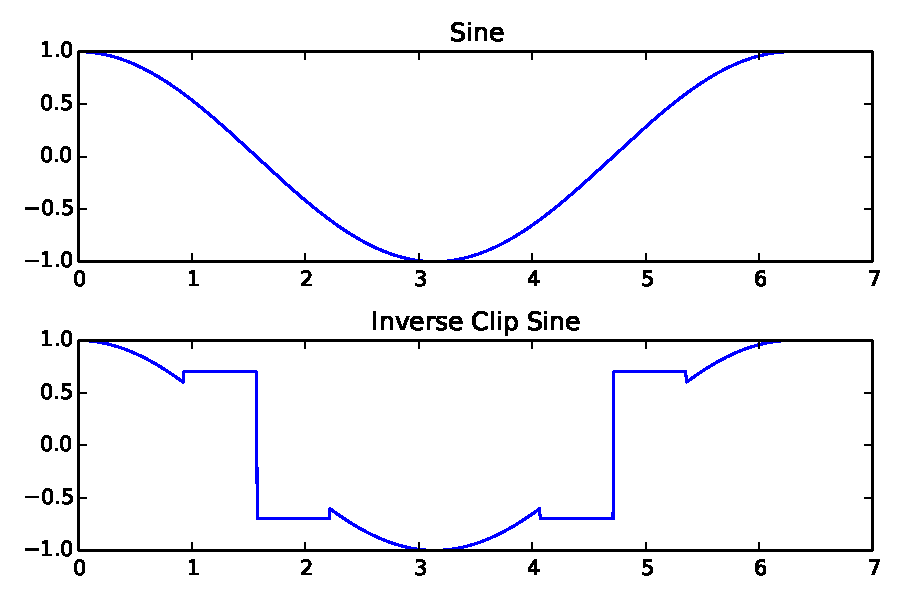
\includegraphics[width=0.8\textwidth]{./pyJvsip_examples/eXinvclip}\captionof{figure}{Inverse Clip Example}
\label{fig:invClipExample}\end{minipage}
\pyComment{
\item{The clip function works much the same as \cvl{} except the output is returned. In line 6 of the example we used the \ttbf{empty} method to create the output vector and saved a reference in the left value.}
\item{The \ttbf{invclip} function is a bit complicated. See the \cvl{} specification for more complete details.}
\item{The \ttbf{view} \ttbf{in} is clipped according to the rules of the function. The clipping checks are set by \ttbf{t1} (low),  \ttbf{t2}(mid), and \ttbf{t3}(high); and the clip values are set by \ttbf{c1} and \ttbf{c2} accordingly. The output is placed in \ttbf{out}. If \ttbf{in==out} then the function is done in-place}
}
\afuncT{jdot}{Complex Vector Conjugate Dot Product}{matrixOperations}
\\ \hspace*{.8cm}For complex vector views $a$ and $b$
\begin{equation*}
\alpha = \sum \limits_{i=0}^{N-1} a_i \cdot \opConj(b_i)
\end{equation*}
\\\cvsiplh
\\ \hspace*{.8cm} \vspace*{.1cm} \textbf{Available Functions }
\\ \hspace*{0.03\textwidth} {
\ttfamily
\begin{tabular}[H]{l}
vsip\_cscalar\_d vsip\_cvjdot\_d(\\*\hspace{.6cm}const vsip\_cvview\_d*, const vsip\_cvview\_d*);\\
vsip\_cscalar\_f vsip\_cvjdot\_f(\\*\hspace{.6cm}const vsip\_cvview\_f*, const vsip\_cvview\_f*);\\
\end{tabular}
}
\\\pyjvsiph
\viewmthd{yes}{No}{NA}{$\alpha$=a.jdot(b)}
\apyfunc{No}{}
\pyComment{\item {For C VSPL only complex vectors are supported. For \pyjv{} \ttbf{jdot} has been extended to support mixed depth vectors.}
\item{Precision of input vectors must agree.}
}
\afuncT{jmul}{Computes the product of a complex \ttbf{view} with the conjugate of a second complex \ttbf{view}, by element.}{binaryOperations}
\\\cvsiplh
\afh
{\ttfamily
\\\hspace*{.04\textwidth}\begin{tabular}[H]{l}
vsip\_cscalar\_d vsip\_cjmul\_d(vsip\_cscalar\_d, vsip\_cscalar\_d);\Bs\\
vsip\_cscalar\_f vsip\_cjmul\_f(vsip\_cscalar\_f, vsip\_cscalar\_f);\Bs\\void vsip\_cmjmul\_d(\\*\hspace{1cm}const vsip\_cmview\_d*, const vsip\_cmview\_d*, const vsip\_cmview\_d*);\Bs\\
void vsip\_cmjmul\_f(\\*\hspace{1cm}const vsip\_cmview\_f*, const vsip\_cmview\_f*, const vsip\_cmview\_f*);\Bs\\
void vsip\_cvjmul\_d(\\*\hspace{1cm}const vsip\_cvview\_d*, const vsip\_cvview\_d*, const vsip\_cvview\_d*);\Bs\\
void vsip\_cvjmul\_f(\\*\hspace{1cm}const vsip\_cvview\_f*, const vsip\_cvview\_f*, const vsip\_cvview\_f*);\Bs\\
\end{tabular}
}
\pyjvsiph
\afunc{jprod}{Matrix conjugate product. \ref{tab:matrixOperations}.}
\\\cvsiplh
\newline \hspace*{.8cm} \vspace*{.1cm} \textbf{Available Functions }
\newline \hspace*{1.1cm} {
\ttfamily
\begin{tabular}[H]{l}
\end{tabular}
}
\\\pyjvsiph

\afuncT{kron}{Kronecker Product}{matrixOperations}
\\\cvsiplh
\\ \hspace*{.8cm} \vspace*{.1cm} \textbf{Available Functions }
\\ \hspace*{0.03\textwidth} {
\ttfamily
\begin{tabular}[H]{l}
void vsip\_cmkron\_d(vsip\_cscalar\_d, const vsip\_cmview\_d *,\\*\hspace{.6cm}const vsip\_cmview\_d *, const vsip\_cmview\_d *);\\
void vsip\_cmkron\_f(vsip\_cscalar\_f, const vsip\_cmview\_f *,\\*\hspace{.6cm}const vsip\_cmview\_f *, const vsip\_cmview\_f *);\\
void vsip\_cvkron\_d(vsip\_cscalar\_d, const vsip\_cvview\_d *,\\*\hspace{.6cm}const vsip\_cvview\_d *, const vsip\_cmview\_d *);\\
void vsip\_cvkron\_f(vsip\_cscalar\_f, const vsip\_cvview\_f *,\\*\hspace{.6cm}const vsip\_cvview\_f *, const vsip\_cmview\_f *);\\
void vsip\_mkron\_d(vsip\_scalar\_d, const vsip\_mview\_d *,\\*\hspace{.6cm}const vsip\_mview\_d *, const vsip\_mview\_d *);\\
void vsip\_mkron\_f(vsip\_scalar\_f, const vsip\_mview\_f *,\\*\hspace{.6cm}const vsip\_mview\_f *, const vsip\_mview\_f *);\\
void vsip\_vkron\_d(vsip\_scalar\_d, const vsip\_vview\_d *,\\*\hspace{.6cm}const vsip\_vview\_d *, const vsip\_mview\_d *);\\
void vsip\_vkron\_f(vsip\_scalar\_f, const vsip\_vview\_f *,\\*\hspace{.6cm}const vsip\_vview\_f *, const vsip\_mview\_f *);\\
\end{tabular}
}
\\\pyjvsiph
\viewmthd{No}{No}{No}{}
\apyfunc{yes}{out = kron(alpha,inOne,inTwo,out)}
\pyComment{
\item The \ttbf{kron} function works much the same as the C VSIPL version except that a 
convenience pointer to the output view is returned. This must be done out-of-place.
}
\afunc{leq}{Computes the boolean comparison of “equal,” by element, of two views.}
\\\cvsiplh
\\\pyjvsiph
\afuncT{lge}{Logical greater than or equal, by element.}{logicalOperations}
\\\cvsiplh
\afh
{
\ttfamily
\\\hspace*{.04\textwidth}\begin{tabular}[H]{l}
void vsip\_mlge\_d(\\*\hspace{1cm}const vsip\_mview\_d*, const vsip\_mview\_d*, const vsip\_mview\_bl*);\\
void vsip\_mlge\_f(\\*\hspace{1cm}const vsip\_mview\_f*, const vsip\_mview\_f*, const vsip\_mview\_bl*);\\
void vsip\_svlge\_f(\\*\hspace{1cm}vsip\_scalar\_f, const vsip\_vview\_f*, const vsip\_vview\_bl*);\\
void vsip\_svlge\_d(\\*\hspace{1cm}vsip\_scalar\_d, const vsip\_vview\_d*, const vsip\_vview\_bl*);\\
void vsip\_vlge\_d(\\*\hspace{1cm}const vsip\_vview\_d*, const vsip\_vview\_d*, const vsip\_vview\_bl*);\\
void vsip\_vlge\_f(\\*\hspace{1cm}const vsip\_vview\_f*, const vsip\_vview\_f*, const vsip\_vview\_bl*);\\
void vsip\_vlge\_i(\\*\hspace{1cm}const vsip\_vview\_i*, const vsip\_vview\_i*, const vsip\_vview\_bl*);\\
void vsip\_vlge\_si(\\*\hspace{1cm}const vsip\_vview\_si*, const vsip\_vview\_si*, const vsip\_vview\_bl*);\\
void vsip\_vlge\_uc(\\*\hspace{1cm}const vsip\_vview\_uc*, const vsip\_vview\_uc*, const vsip\_vview\_bl*);\\
\end{tabular}
}
\\\pyjvsiph
\viewmthd{Yes}{No}{No}{out=in.lge(arg)}
\apyfunc{Yes}{out = lge(in1,in2,out)}
\pyComment{
\item{For return value \ttbf{out} precision is of type \ttbf{\_bl} and shape is compliant with input \ttbf{view}s.}
\item{For method check is \ttbf{in >= arg} and for function check is \ttbf{in1 >= in2}.}
\item{For functions input \ttbf{in1} may be scalar for precisions of type \ttbf{\_f} and \ttbf{\_d} with vector shape. Other options are defined but have not been done for \jv{} at this time. The function will complain if comparisons are not available.}
\item{For methods if input \ttbf{arg} is a scalar it is converted to a constant vector with one element, stride of zero, and compliant length before the comparison. For this reason the \ttbf{view} method will work for some cases the function does not.
}
\item{One needs to be careful. The function call \ttbf{lge(aScalar,aVector,out)} is not the same as \ttbf{aVector.lge(aScalar)}. The first case checks if \ttbf{aScalar >= aVector} and the second case checks if \ttbf{aVector >= aScalar}}
}
\afunc{lgt}{Logical Greater Than}
\\\cvsiplh
\\\pyjvsiph
\afuncT{linear}{Returns the mean value of all the elements of a view.}{unaryOperations}
\\\cvsiplh
\newline \hspace*{.8cm} \vspace*{.1cm} \textbf{Available Functions }
\newline \hspace*{1.1cm} {
\ttfamily
\begin{tabular}[H]{l}
void vsip\_minterp\_linear\_f ( const vsip\_vview\_f *, const vsip\_mview\_f *, vsip\_major, const vsip\_vview\_f *, const vsip\_mview\_f * ) ;\\
void vsip\_vinterp\_linear\_f ( const vsip\_vview\_f *, const vsip\_vview\_f *, const vsip\_vview\_f *, const vsip\_vview\_f * ) ;\\
void vsip\_minterp\_linear\_d ( const vsip\_vview\_d *, const vsip\_mview\_d *, vsip\_major, const vsip\_vview\_d *, const vsip\_mview\_d * ) ;\\
void vsip\_vinterp\_linear\_d( const vsip\_vview\_d *, const vsip\_vview\_d *, const vsip\_vview\_d *, const vsip\_vview\_d *);\\
\end{tabular}
}\\
\\\pyjvsiph
\viewmthd{Yes}{Yes}{NA}{msq=in.meansqval}
\apyfunc{No}{NA}
\pyComment{\item{There seemed to be no reason to include this as a separate function for \pyjv}}
\afuncT{lle}{Logical less than or equal}{logicalOperations}
\\\cvsiplh
\\\pyjvsiph
\afuncT{llsqsol}{Solve linear least squares problem.}{specialLinearSystemSolvers}
\\\cvsiplh
\\ \hspace*{.8cm} \vspace*{.1cm} \textbf{Available Functions }
\\ \hspace*{1.1cm} {
\ttfamily
\begin{tabular}[H]{l}
\end{tabular}
}
\\\pyjvsiph

\afuncT{llt}{Logical less than.}{logicalOperations}
\afh
{
\ttfamily
\\\hspace*{.04\textwidth}\begin{tabular}[H]{l}
void vsip\_mllt\_d(\\*\hspace{1cm}const vsip\_mview\_d*, const vsip\_mview\_d*, const vsip\_mview\_bl*);\\
void vsip\_mllt\_f(\\*\hspace{1cm}const vsip\_mview\_f*, const vsip\_mview\_f*, const vsip\_mview\_bl*);\\
void vsip\_svllt\_f(\\*\hspace{1cm}vsip\_scalar\_f, const vsip\_vview\_f*, const vsip\_vview\_bl*);\\
void vsip\_svllt\_d(\\*\hspace{1cm}vsip\_scalar\_d, const vsip\_vview\_d*, const vsip\_vview\_bl*);\\
void vsip\_vllt\_d(\\*\hspace{1cm}const vsip\_vview\_d*, const vsip\_vview\_d*, const vsip\_vview\_bl*);\\
void vsip\_vllt\_f(\\*\hspace{1cm}const vsip\_vview\_f*, const vsip\_vview\_f*, const vsip\_vview\_bl*);\\
void vsip\_vllt\_i(\\*\hspace{1cm}const vsip\_vview\_i*, const vsip\_vview\_i*, const vsip\_vview\_bl*);\\
void vsip\_vllt\_si(\\*\hspace{1cm}const vsip\_vview\_si*, const vsip\_vview\_si*, const vsip\_vview\_bl*);\\
void vsip\_vllt\_uc(\\*\hspace{1cm}const vsip\_vview\_uc*, const vsip\_vview\_uc*, const vsip\_vview\_bl*);\\
\end{tabular}
}
\\\cvsiplh
\\\pyjvsiph
\viewmthd{Yes}{No}{No}{out=in.llt(arg)}
\apyfunc{Yes}{out = llt(in1,in2,out)}
\pyComment{
\item{For return value \ttbf{out} precision is of type \ttbf{\_bl} and shape is compliant with input \ttbf{view}s.}
\item{For method check is \ttbf{in < arg} and for function check is \ttbf{in1 < in2}.}
\item{For functions input \ttbf{in1} may be scalar for precisions of type \ttbf{\_f} and \ttbf{\_d} with vector shape. Other options are defined but have not been done for \jv{} at this time. The function will complain if comparisons are not available.}
\item{For methods if input \ttbf{arg} is a scalar it is converted to a constant vector with one element, stride of zero, and compliant length before the comparison. For this reason the \ttbf{view} method will work for some cases the function does not.
}
\item{One needs to be careful. The function call \ttbf{llt(aScalar,aVector,out)} is not the same as \ttbf{aVector.llt(aScalar)}. The first case checks if \ttbf{aScalar < aVector} and the second case checks if \ttbf{aVector < aScalar}}
}
\afuncT{lne}{Logical not equal}{logicalOperations}
\\\cvsiplh
\afh
{
\ttfamily
\\\hspace*{.04\textwidth}\begin{tabular}[H]{l}
void vsip\_mlne\_d(\\*\hspace{1cm}const vsip\_mview\_d*, const vsip\_mview\_d*, const vsip\_mview\_bl*);\\
void vsip\_mlne\_f(\\*\hspace{1cm}const vsip\_mview\_f*, const vsip\_mview\_f*, const vsip\_mview\_bl*);\\
void vsip\_svlne\_f(\\*\hspace{1cm}vsip\_scalar\_f, const vsip\_vview\_f*, const vsip\_vview\_bl*);\\
void vsip\_svlne\_d(\\*\hspace{1cm}vsip\_scalar\_d, const vsip\_vview\_d*, const vsip\_vview\_bl*);\\
void vsip\_vlne\_d(\\*\hspace{1cm}const vsip\_vview\_d*, const vsip\_vview\_d*, const vsip\_vview\_bl*);\\
void vsip\_vlne\_f(\\*\hspace{1cm}const vsip\_vview\_f*, const vsip\_vview\_f*, const vsip\_vview\_bl*);\\
void vsip\_vlne\_i(\\*\hspace{1cm}const vsip\_vview\_i*, const vsip\_vview\_i*, const vsip\_vview\_bl*);\\
void vsip\_vlne\_si(\\*\hspace{1cm}const vsip\_vview\_si*, const vsip\_vview\_si*, const vsip\_vview\_bl*);\\
void vsip\_vlne\_uc(\\*\hspace{1cm}const vsip\_vview\_uc*, const vsip\_vview\_uc*, const vsip\_vview\_bl*);\\
\end{tabular}
}
\\\pyjvsiph
\viewmthd{Yes}{No}{No}{out=in.lne(arg)}
\apyfunc{Yes}{out = lne(in1,in2,out)}
\pyComment{
\item{For return value \ttbf{out} precision is of type \ttbf{\_bl} and shape is compliant with input \ttbf{view}s.}
\item{For method check is \ttbf{in != arg} and for function check is \ttbf{in1 != in2}.}
\item{For functions input \ttbf{in1} may be scalar for precisions of type \ttbf{\_f} and \ttbf{\_d} with vector shape. Other options are defined but have not been done for \jv{} at this time. The function will complain if comparisons are not available.}
\item{For methods if input \ttbf{arg} is a scalar it is converted to a constant vector with one element, stride of zero, and compliant length before the comparison. For this reason the \ttbf{view} method will work for some cases the function does not.}
}
\afuncT{log10}{Compute the base ten logarithm; An element-wise function.}{elementaryMath}
\\\cvsiplh
\\ \hspace*{.8cm} \vspace*{.1cm} \textbf{Available Functions }
\\ \hspace*{1.1cm} {
\ttfamily
\begin{tabular}[H]{l}
vsip\_scalar\_d vsip\_log10\_d(vsip\_scalar\_d)\\
vsip\_scalar\_f vsip\_log10\_f(vsip\_scalar\_f)\\
void vsip\_mlog10\_d(\\*\hspace{1cm}const vsip\_mview\_d*, const vsip\_mview\_d*);\\
void vsip\_mlog10\_f(\\*\hspace{1cm}const vsip\_mview\_f*, const vsip\_mview\_f*);\\
void vsip\_vlog10\_d(\\*\hspace{1cm}const vsip\_vview\_d*, const vsip\_vview\_d*);\\
void vsip\_vlog10\_f(\\*\hspace{1cm}const vsip\_vview\_f*, const vsip\_vview\_f*);\\
\end{tabular}
}
\\\pyjvsiph
\viewmthd{yes}{yes}{yes}{inOut.log10}
\apyfunc{yes}{out = log10(in,out)}
\\ \hspace*{1.2cm}\parbox{10.8cm}{\vspace*{.1cm}The \ttbf{log10} function works much the same as the C VSIPL version except that a convenience pointer to the output view is returned. This may be done in-place if \ttbf{in==out}.}

\afuncT{log}{Natural logarithm; An element-wise function.}{elementaryMath}
\\\cvsiplh
\newline \hspace*{.8cm} \vspace*{.1cm} \textbf{Available Functions }
\newline \hspace*{1.1cm} {
\ttfamily
\begin{tabular}[H]{l}
\end{tabular}
}
\\\pyjvsiph
\viewmthd{yes}{yes}{yes}{inOut.sin}
\apyfunc{yes}{out = sin(in,out)}
\newline\hspace*{1.2cm}\parbox{10.8cm}{\vspace*{.1cm}The \ttbf{log} function works much the same as the C VSIPL version except that a convenience pointer to the output view is returned. This may be done in-place if \ttbf{in==out}.}

\clearpage
\hypertarget{ludFunc}{\large \textbf{LUD Function Set}}\hspace*{\fill}(up)\vspace{.2cm}\\
\hspace*{.3cm}
\parbox{0.85\textwidth}{Lower-Upper Decomposition Class. \ref{tab:generalSquareSolver}}
\\\cvsiplh 
\newline \hspace*{.8cm} \vspace*{.1cm} \textbf{Available Functions }
%
%\newline \hspace*{.8cm} \vspace*{.1cm} \texttt{lud\_create}
\newline \hspace*{1.cm} {
\ttfamily\vspace{.3cm}
\begin{tabular}[H]{|l|}
\multicolumn{1}{c}{\rmfamily \bfseries Create LU Object\vspace{.1cm}}\\ \hline
vsip\_lu\_d* vsip\_lud\_create\_d(vsip\_length);\\
vsip\_lu\_f* vsip\_lud\_create\_f(vsip\_length);\\
vsip\_clu\_d* vsip\_clud\_create\_d(vsip\_length);\\
vsip\_clu\_f* vsip\_clud\_create\_f(vsip\_length);\\
\hline\end{tabular}\\}
%
%\newline \hspace*{.8cm} \vspace*{.1cm} \texttt{lud\_destroy}
\newline \hspace*{1.cm} {
\ttfamily\vspace{.3cm}
\begin{tabular}[H]{|l|}
\multicolumn{1}{c}{\rmfamily \bfseries Destroy LU Object\vspace{.1cm}}\\ \hline
int vsip\_lud\_destroy\_d(vsip\_lu\_d*);\\
int vsip\_lud\_destroy\_f(vsip\_lu\_f*);\\
int vsip\_clud\_destroy\_d(vsip\_clu\_d*);\\
int vsip\_clud\_destroy\_f(vsip\_clu\_f*);\\
\hline\end{tabular}\\}
%
%\newline \hspace*{.8cm} \vspace*{.1cm} \texttt{lud}
\newline \hspace*{1.cm}{
\ttfamily\vspace{.3cm}
\begin{tabular}[H]{|l|}
\multicolumn{1}{c}{\rmfamily \bfseries Calculate LU Decomposition\vspace{.1cm}}\\ \hline
int vsip\_lud\_d(vsip\_lu\_d*, const vsip\_mview\_d*);\\
int vsip\_lud\_f(vsip\_lu\_f*, const vsip\_mview\_f*);\\
int vsip\_clud\_d(vsip\_clu\_d*, const vsip\_cmview\_d*);\\
int vsip\_clud\_f(vsip\_clu\_f*, const vsip\_cmview\_f*);\\
\hline\end{tabular}\\}
%
%\newline \hspace*{.8cm} \vspace*{.1cm} \texttt{lusol}\\
\newline \hspace*{1.cm}{
\ttfamily\vspace{.3cm}
\begin{tabular}[H]{|l|}
\multicolumn{1}{c}{\rmfamily \bfseries Solve Using Calculated LU Decomposition\vspace{.1cm}}\\ \hline
int vsip\_lusol\_d(const vsip\_lu\_d*, vsip\_mat\_op,\\*\hspace*{.8cm} const vsip\_mview\_d*);\\
int vsip\_lusol\_f(const vsip\_lu\_f*, vsip\_mat\_op,\\*\hspace*{.8cm} const vsip\_mview\_f*);\\
int vsip\_clusol\_d(const vsip\_clu\_d*, vsip\_mat\_op,\\*\hspace*{.8cm} const vsip\_cmview\_d*);\\
int vsip\_clusol\_f(const vsip\_clu\_f*, vsip\_mat\_op,\\*\hspace*{.8cm} const vsip\_cmview\_f*);\\
\hline\end{tabular}\\}
%
%\newline \hspace*{.8cm} \vspace*{.1cm} \texttt{lud\_getattr}
\newline \hspace*{1.cm}{
\ttfamily\vspace{.3cm}
\begin{tabular}[H]{|l|}
\multicolumn{1}{c}{\rmfamily \bfseries Fill LU Attribute Structure\vspace{.1cm}}\\ \hline
void vsip\_lud\_getattr\_d(const vsip\_lu\_d*,\\*\hspace*{.8cm} vsip\_lu\_attr\_d*);\\
void vsip\_lud\_getattr\_f(const vsip\_lu\_f*,\\*\hspace*{.8cm} vsip\_lu\_attr\_f*);\\
void vsip\_clud\_getattr\_d(const vsip\_clu\_d*,\\*\hspace*{.8cm} vsip\_clu\_attr\_d*);\\
void vsip\_clud\_getattr\_f(const vsip\_clu\_f*,\\*\hspace*{.8cm} vsip\_clu\_attr\_f*);\\
\hline\end{tabular}\\}
%
\clearpage\pyjvsiph
\newline\hspace*{.8cm}{\textbf{View Methods\vspace{.2cm}}\\
\hspace*{1cm}\parbox{10.5cm}{
\begin{itemize}
\item {A \ttbf{view} method has been defined for the kernel \ttbf{view}. The kernel is treated as non-symmetric so the entire kernel is assumed.\footnotemark[1]}
\item {A variable argument list is supported.} 
\subitem{The first required argument is the input data \ttbf{view}.}
\subitem {\parbox[t]{.74\textwidth}{The second optional argument is the decimation factor. It defaults to one.}\vspace*{.1cm}}
\item{Other parameters are either set to there default value, or are calculated from included parameters.\vspace{.2cm}}
\end{itemize}}\\
\hspace*{1.cm}\textbf{In-Place: }\hspace{.2cm} no\\
\hspace*{1.1cm}\textbf{Out-Of-Place: }\hspace{.2cm} yes\\
\hspace*{1.1cm}\textbf{Example: }\vspace*{.1cm}\\
\hspace*{1.cm}\parbox[t]{.85\textwidth}{
\begin{tabular}[t]{|l l|}
\multicolumn{2}{c}{\parbox[t]{.68\textwidth}{\center{\rmfamily \bfseries Finite Impulse Response Argument List\vspace{.2cm}}}}\\ \hline
\ttbf{filt} & \parbox[t]{.74\textwidth}{A vector \ttbf{view} of filter coefficients.\\*Required argument \vspace*{.1cm}}\\ \hline
\ttbf{sym} & \parbox[t]{.74\textwidth}{Symmetry of \ttbf{filt} kernel. \\* Required argument\vspace*{.1cm}} \\\hline
\ttbf{N} & \parbox[t]{.74\textwidth}{Length of input data vector. \\* Required argument\vspace*{.1cm}}\\\hline
\ttbf{D} & \parbox[t]{.74\textwidth}{Decimation factor.\\* Required argument\vspace*{.1cm}}\\\hline
\ttbf{state} & \parbox[t]{.74\textwidth}{Flag to indicate if the filter state is to be saved.\\*
\ttbf{VSIP\_STATE\_SAVE} or \ttbf{VSIP\_STATE\_NO\_SAVE}\\* Argument is supported but defaults to not saving. \\* Instead of \ttbf{VSIP} flags you may use the strings \ttbf{'YES'} or \ttbf{'NO'}.\vspace*{.1cm}}\\ \hline
\ttbf{ntimes} & \parbox[t]{.74\textwidth}{Hint for how much the LUD object will be used. Zero indicates many times.\\*For \jv{} this argument is only supported at the interface level and defaults to zero.\vspace*{.1cm}} \\\hline
\ttbf{algHint} & \parbox[t]{.74\textwidth}{Algorithm hint to optimize for\\*speed (\ttbf{VSIP\_ALG\_TIME}),\\*size (\ttbf{VSIP\_ALG\_SPACE}),\\* or accuracy (\ttbf{VSIP\_ALG\_NOISE}).\\*For \jv{} this argument is only supported at the interface level and defaults to time.\vspace*{.1cm}}\\
\hline \end{tabular}\\
\begin{tabular}{|l l|}
\multicolumn{2}{c}{\parbox[t]{.68\textwidth}{\center{\rmfamily \bfseries Finite Impulse Response Filter Types\vspace{.2cm}}}}\\ \hline
'fir\_f' & \parbox[t]{.68\textwidth}{Real \ttbf{LUD}; float precision \vspace*{.1cm}}\\\hline
'cfir\_f' & \parbox[t]{.68\textwidth}{ Complex \ttbf{LUD}; float precision \vspace*{.1cm}}\\\hline
'rcfir\_f' & \parbox[t]{.68\textwidth}{ Complex \ttbf{LUD} with real \ttbf{kernel}; float precision \vspace*{.1cm}}\\\hline
'fir\_d' & \parbox[t]{.68\textwidth}{ Real \ttbf{LUD}; double precision \vspace*{.1cm}}\\\hline
'cfir\_d' & \parbox[t]{.68\textwidth}{Complex \ttbf{LUD}; double precision \vspace*{.1cm}}\\\hline
'rcfir\_d' & \parbox[t]{.68\textwidth}{Complex \ttbf{LUD} with real \ttbf{kernel}; double precision \vspace*{.1cm}}\\\hline
\end{tabular}\vspace*{.4cm}}\\
\clearpage
%
\hspace*{.8cm}{\textbf{LUD Class Methods}\\
\hspace*{1.1cm} \parbox[t]{.88\textwidth}{For class methods table we assume we have created an LUD object we call \ttbf{firObj} and we have an input \ttbf{view x} compliant with \ttbf{firObj} and a compliant output \ttbf{view y}.\vspace{.2cm}}
\newline
\hspace*{1.cm}\parbox[t]{.85\textwidth}{\begin{tabular}{|l l|}
\multicolumn{2}{c}{\parbox[t]{.58\textwidth}{\center{\rmfamily \bfseries Finite Impulse Response Filter Methods\vspace{.2cm}}}}\\ \hline
\ttbf{firObj.flt(x,y)} & \parbox[t]{.58\textwidth}{Filter the data \ttbf{x} and place the results in \ttbf{y}}\\\hline
\ttbf{firObj.decimation} & \parbox[t]{.58\textwidth}{ Returns integer decimation factor. \vspace*{.1cm}}\\\hline
\ttbf{firObj.length} & \parbox[t]{.58\textwidth}{ Returns integer length for \ttbf{x}. \vspace*{.1cm}}\\\hline
\ttbf{firObj.lengthOut} & \parbox[t]{.58\textwidth}{ Returns integer of valid data points in \ttbf{y} \vspace*{.1cm}}\\\hline
\ttbf{firObj.reset} & \parbox[t]{.58\textwidth}{Resets LUD filter to it's initial state. \vspace*{.1cm}}\\\hline
\ttbf{firObj.state} & \parbox[t]{.58\textwidth}{Returns \ttbf{True} if filter state is saved, otherwise returns \ttbf{False}.\vspace*{.1cm}}\\\hline
\ttbf{firObj.type} & \parbox[t]{.58\textwidth}{Returns string indicating filter type.\vspace*{.1cm}}\\\hline
\ttbf{firObj.vsip} & \parbox[t]{.58\textwidth}{Returns C VSIPL filter instance.\vspace*{.1cm}}\\\hline
\end{tabular}\vspace*{.4cm}}\\
\hspace*{.7cm} \parbox[t]{.91\textwidth}{
\begin{itemize}
\item{Methods \ttbf{decimation}, \ttbf{length}, \ttbf{state}, \ttbf{type} and \ttbf{vsip} are set when the LUD instance is created and do not change after create}
\item{Method \ttbf{lengthOut}\footnotemark[2] is calculated during the execution of method \ttbf{flt(x,y)} and is useful if state is saved and the filter object is used multiple times on a long piece of data.}
\item{Method \ttbf{reset} is used if state is saved and the filter is used multiple times on a long data set and then \emph{reset}\footnotemark[3] to it's initial state for use on multiple long data sets.}
\end{itemize}}
\footnotetext[1]{This does not preclude symmetric kernels. You just need the entire kernel.}
\footnotetext[2]{See C VSIPL specification for more information on length of output data.}
\footnotetext[3]{See signal processing text on overlap-add and overlap-save filtering.}

\afuncT{ma}{Multiply and add. An element-wise function.}{ternaryOperations}
\\\cvsiplh
\afh
{
\ttfamily
\\\hspace*{.04\textwidth}\begin{tabular}[H]{l}
void vsip\_cvma\_d(const vsip\_cvview\_d*, const vsip\_cvview\_d*,\\*\hspace{.7cm}const vsip\_cvview\_d*, const vsip\_cvview\_d*);\\
void vsip\_cvma\_f(const vsip\_cvview\_f*, const vsip\_cvview\_f*,\\*\hspace{.7cm}const vsip\_cvview\_f*, const vsip\_cvview\_f*);\\
void vsip\_cvsma\_d(const vsip\_cvview\_d*, vsip\_cscalar\_d,\\*\hspace{.7cm}const vsip\_cvview\_d*, const vsip\_cvview\_d*);\\
void vsip\_cvsma\_f(const vsip\_cvview\_f*, vsip\_cscalar\_f,\\*\hspace{.7cm}const vsip\_cvview\_f*, const vsip\_cvview\_f*);\\
void vsip\_vma\_d(const vsip\_vview\_d*, const vsip\_vview\_d*,\\*\hspace{.7cm}const vsip\_vview\_d*, const vsip\_vview\_d*);\\
void vsip\_vma\_f(const vsip\_vview\_f*, const vsip\_vview\_f*,\\*\hspace{.7cm}const vsip\_vview\_f*, const vsip\_vview\_f*);\\
void vsip\_vsma\_d(const vsip\_vview\_d*, vsip\_scalar\_d,\\*\hspace{.7cm}const vsip\_vview\_d*, const vsip\_vview\_d*);\\
void vsip\_vsma\_f(const vsip\_vview\_f*, vsip\_scalar\_f,\\*\hspace{.7cm}const vsip\_vview\_f*, const vsip\_vview\_f*);\\
void vsip\_cvsmsa\_d(const vsip\_cvview\_d*, vsip\_cscalar\_d,\\*\hspace{.7cm}vsip\_cscalar\_d, const vsip\_cvview\_d*);\\
void vsip\_cvsmsa\_f(const vsip\_cvview\_f*, vsip\_cscalar\_f,\\*\hspace{.7cm}vsip\_cscalar\_f, const vsip\_cvview\_f*);\\
void vsip\_vsmsa\_d(const vsip\_vview\_d*, vsip\_scalar\_d,\\*\hspace{.7cm}vsip\_scalar\_d, const vsip\_vview\_d*);\\
void vsip\_vsmsa\_f(const vsip\_vview\_f*, vsip\_scalar\_f,\\*\hspace{.7cm}vsip\_scalar\_f, const vsip\_vview\_f*);\\
\end{tabular}
}
\pyComment{
\item{The C VSIPL spec has separate man pages for multiply-add functions containing scalar arguments, and those containing only \ttbf{view} arguments.}}
\\\pyjvsiph
\viewmthd{No}{NA}{NA}{NA}
\apyfunc{yes}{\ttbf{out = ma(in1,in2,in3,out)}}
\pyComment{
\item{Argument \ttbf{in1} is always a \ttbf{view}, argument \ttbf{in2} is either a \ttbf{view} or a scalar and argument \ttbf{in3} is either a \ttbf{view} or a scalar.}
\item{The \ttbf{ma} function works much the same as the C VSIPL version except that a convenience pointer to the output \ttbf{view} is returned.}
\item{This may be done in-place if an input \ttbf{view} is the same as the output \ttbf{view}.}}
\afuncT{mag}{Arctangent of Two Arguments; An elementwise function}{unaryOperations}
\\\cvsiplh
\\\pyjvsiph
\afuncT{magsq}{Arctangent of Two Arguments; An elementwise function}{unaryOperations}
\\\cvsiplh
\afh
\\\hspace*{.04\textwidth} {
\ttfamily
}
\\\pyjvsiph
\afunc{max}{Maximum}
\\\cvsiplh
\\\pyjvsiph
\afuncT{maxmg}{Maximum Magnitude}{selectionOperations}
\\\cvsiplh
\afh
{
\ttfamily
\\\hspace*{.04\textwidth}\begin{tabular}[H]{l}
\end{tabular}
}
\\\pyjvsiph
%
\viewmthd{No}{NA}{NA}{NA}
%
\apyfunc{No}{NA}
%
\pyComment{
\item{No comments}
}
\afuncT{maxmgsq}{Maximum Magnitude of the Square}{selectionOperations}
\\\cvsiplh
\\\pyjvsiph
 afunc{maxmgval}{Maximum Magnitude Value}
\\\cvsiplh
\\\pyjvsiph
 afunc{maxval}{Maximum Value}
\\\cvsiplh
\\\pyjvsiph
\afuncT{meansqval}{Returns the mean value of all the elements of a view.}{unaryOperations}
\\\cvsiplh
\newline \hspace*{.8cm} \vspace*{.1cm} \textbf{Available Functions }
\newline \hspace*{1.1cm} {
\ttfamily
\begin{tabular}[H]{l}
vsip\_scalar\_d vsip\_cmmeansqval\_d(const vsip\_cmview\_d*);\\
vsip\_scalar\_d vsip\_cvmeansqval\_d(const vsip\_cvview\_d*);\\
vsip\_scalar\_d vsip\_mmeansqval\_d(const vsip\_mview\_d*);\\
vsip\_scalar\_d vsip\_vmeansqval\_d(const vsip\_vview\_d*);\\
vsip\_scalar\_f vsip\_cmmeansqval\_f(const vsip\_cmview\_f*);\\
vsip\_scalar\_f vsip\_cvmeansqval\_f(const vsip\_cvview\_f*);\\
vsip\_scalar\_f vsip\_mmeansqval\_f(const vsip\_mview\_f*);\\
vsip\_scalar\_f vsip\_vmeansqval\_f(const vsip\_vview\_f*);\\
\end{tabular}
}
\\\pyjvsiph
\viewmthd{Yes}{Yes}{NA}{msq=in.meansqval}
\apyfunc{No}{NA}
\pyComment{\item{There seemed to be no reason to include this as a separate function for \pyjv}}
\afuncT{meanval}{Returns the mean value of all the elements of a view.}{unaryOperations}
\\\cvsiplh
\afh
\\\hspace*{.04\textwidth} {
\ttfamily
\begin{tabular}[H]{l}
vsip\_cscalar\_d vsip\_cmmeanval\_d(const vsip\_cmview\_d*);\\
vsip\_cscalar\_d vsip\_cvmeanval\_d(const vsip\_cvview\_d*);\\
vsip\_cscalar\_f vsip\_cmmeanval\_f(const vsip\_cmview\_f*);\\
vsip\_cscalar\_f vsip\_cvmeanval\_f(const vsip\_cvview\_f*);\\
vsip\_scalar\_d vsip\_mmeanval\_d(const vsip\_mview\_d*);\\
vsip\_scalar\_d vsip\_vmeanval\_d(const vsip\_vview\_d*);\\
vsip\_scalar\_f vsip\_mmeanval\_f(const vsip\_mview\_f*);\\
vsip\_scalar\_f vsip\_vmeanval\_f(const vsip\_vview\_f*);\\
\end{tabular}
}
\\\pyjvsiph
\viewmthd{Yes}{Yes}{NA}{m=in.meanval}
\apyfunc{No}{NA}
\pyComment{\item{There seemed to be no reason to include this as a separate function for \pyjv}}
\afuncT{min}{Minimum}{selectionOperations}
\\\cvsiplh
\afh
{
\ttfamily
\\\hspace*{.04\textwidth}\begin{tabular}[H]{l}
\end{tabular}
}
\\\pyjvsiph
\afuncT{minmg}{Minimum Magnitude}{selectionOperations}
\\\cvsiplh
\\\pyjvsiph
\afuncT{minmnsq}{Minimum Magnitude Square}{selectionOperations}
\\\cvsiplh
\afh
{
\ttfamily
\\\hspace*{.04\textwidth}\begin{tabular}[H]{l}
\end{tabular}
}
\\\pyjvsiph
%
\viewmthd{No}{NA}{NA}{NA}
%
\apyfunc{No}{NA}
%
\pyComment{
\item{No comments}
}
\afuncT{minmgsqval}{Minimum Magnitude Square Value}{selectionOperations}
\\\cvsiplh
\afh
{
\ttfamily
\\\hspace*{.04\textwidth}\begin{tabular}[H]{l}
\end{tabular}
}
\\\pyjvsiph
\afuncT{minmgval}{Minimum Magnitude Value}{selectionOperations}
\\\cvsiplh
\afh
{
\ttfamily
\\\hspace*{.04\textwidth}\begin{tabular}[H]{l}
vsip\_scalar\_d vsip\_mminmgval\_d(const vsip\_mview\_d*, vsip\_scalar\_mi*);\\
vsip\_scalar\_d vsip\_vminmgval\_d(const vsip\_vview\_d*, vsip\_index *);\\
vsip\_scalar\_f vsip\_mminmgval\_f(const vsip\_mview\_f*, vsip\_scalar\_mi*);\\
vsip\_scalar\_f vsip\_vminmgval\_f(const vsip\_vview\_f*, vsip\_index *);\\
\end{tabular}
}
\\\pyjvsiph
%
\viewmthd{No}{NA}{NA}{NA}
%
\apyfunc{No}{NA}
%
\pyComment{
\item{No comments}
}
\afuncT{minval}{Minimum Value}{selectionOperations}
\\\cvsiplh
\afh
{
\ttfamily
\\\hspace*{.04\textwidth}\begin{tabular}[H]{l}
\end{tabular}
}
\\\pyjvsiph
\afuncT{vmmul}{Vector-Matrix elementwise multiply by row or column.}{binaryOperations}
\\\cvsiplh
\afh
{\ttfamily
\\\hspace*{.04\textwidth}\begin{tabular}[H]{l}
void vsip\_cvmmul\_d(const vsip\_cvview\_d*,\\*\hspace*{1cm}const vsip\_cmview\_d*, vsip\_major, const vsip\_cmview\_d*);\Bs\\
void vsip\_cvmmul\_f(const vsip\_cvview\_f*,\\*\hspace*{1cm}const vsip\_cmview\_f*, vsip\_major, const vsip\_cmview\_f*);\Bs\\
void vsip\_vmmul\_d(const vsip\_vview\_d*,\\*\hspace*{1cm}const vsip\_mview\_d*, vsip\_major, const vsip\_mview\_d*);\Bs\\
void vsip\_vmmul\_f(const vsip\_vview\_f*,\\*\hspace*{1cm}const vsip\_mview\_f*, vsip\_major, const vsip\_mview\_f*);\Bs\\
\end{tabular}
}
\\\pyjvsiph
\afuncT{modulate}{Computes the modulation of a real vector by a specified complex frequency.}{unaryOperations}
\\\cvsiplh
\afh
\\\hspace*{.04\textwidth} {
\ttfamily
\begin{tabular}[H]{l}
vsip\_scalar\_d vsip\_cvmodulate\_d(\\*\hspace{.6cm}const vsip\_cvview\_d*, vsip\_scalar\_d, \\*\hspace{.6cm}vsip\_scalar\_d, const vsip\_cvview\_d*);\\
vsip\_scalar\_d vsip\_vmodulate\_d(\\*\hspace{.6cm}const vsip\_vview\_d*, vsip\_scalar\_d, \\*\hspace{.6cm}vsip\_scalar\_d, const vsip\_cvview\_d*);\\
vsip\_scalar\_f vsip\_cvmodulate\_f(\\*\hspace{.6cm}const vsip\_cvview\_f*, vsip\_scalar\_f, \\*\hspace{.6cm}vsip\_scalar\_f, const vsip\_cvview\_f*);\\
vsip\_scalar\_f vsip\_vmodulate\_f(\\*\hspace{.6cm}const vsip\_vview\_f*, vsip\_scalar\_f, \\*\hspace{.6cm}vsip\_scalar\_f, const vsip\_cvview\_f*);\\
\end{tabular}
}
\\\pyjvsiph
\viewmthd{No}{NA}{NA}{NA}
\apyfunc{Yes}{phiNew,out=modulate(in,nu,phi,out)}
\pyComment{{\item{Note \ttbf{phi} is the initial phase and the final phase is returned as \ttbf{phiNew}. For \pyjv we also return a convenience copy of the output vector}}}
\afunc{msb}{Multiply and subtract. An element-wise function. See ternary functions table \ref{tab:ternaryOperations}.}
\cvsiplh
\newline \hspace*{.8cm} \vspace*{.1cm} \textbf{Available Functions }
\newline \hspace*{1.1cm} {
\ttfamily
\begin{tabular}[H]{l}

\end{tabular}
}
\pyjvsiph
\viewmthd{No}{NA}{NA}{NA}
\apyfunc{yes}{out = msb(in1,in2,in3,out)}
\newline\hspace*{1.2cm}\parbox{10.8cm}{\vspace*{.1cm}The \ttbf{log} function works much the same as the C VSIPL version except that a convenience pointer to the output view is returned. This may be done in-place if \ttbf{in==out}.}
\afuncT{mul}{computes the difference of a scalar and a \ttbf{view} or between two \ttbf{view}s. A binary operation.}{binaryOperations}
\\\cvsiplh
\\\pyjvsiph
\afuncT{nearest}{Nearest Interpolation}{interpolation}
\\\cvsiplh
\newline \hspace*{.8cm} \vspace*{.1cm} \textbf{Available Functions }
\newline \hspace*{1.1cm} {
\ttfamily
\begin{tabular}[H]{l}
void vsip\_vinterp\_nearest\_f(\\*\hspace*{1cm}const vsip\_vview\_f *, const vsip\_vview\_f *,
\\*\hspace*{1cm}const vsip\_vview\_f *, const vsip\_vview\_f*);\\
void vsip\_vinterp\_nearest\_d(\\*\hspace*{1cm}const vsip\_vview\_d *, const vsip\_vview\_d *,
\\*\hspace*{1cm}const vsip\_vview\_d *, const vsip\_vview\_d*);\\
void vsip\_minterp\_nearest\_f(\\*\hspace*{1cm}const vsip\_vview\_f *, const vsip\_mview\_f *,
\\*\hspace*{1cm}vsip\_major, const vsip\_vview\_f *, const vsip\_mview\_f*);\\
void vsip\_minterp\_nearest\_d(\\*\hspace*{1cm}const vsip\_vview\_d*, const vsip\_mview\_d*,
\\*\hspace*{1cm}vsip\_major, const vsip\_vview\_d*, const vsip\_mview\_d*);\\
\end{tabular}
}\\
\\\pyjvsiph

\afunc{neg}{Computes the reciprocal for each element of a \ttbf{view}. An elementwise function. See unary operations table \ref{tab:unaryOperations}}
\cvsiplh
\newline \hspace*{.8cm} \vspace*{.1cm} \textbf{Available Functions }
\newline \hspace*{1.1cm} {
\ttfamily
\begin{tabular}[H]{l}
vsip\_cscalar\_d vsip\_cneg\_d(vsip\_cscalar\_d);\\
vsip\_cscalar\_f vsip\_cneg\_f(vsip\_cscalar\_f);\\
void vsip\_cmneg\_d(\\*\hspace{.6cm}const vsip\_cmview\_d*, const vsip\_cmview\_d*);\\
void vsip\_cmneg\_f(\\*\hspace{.6cm}const vsip\_cmview\_f*, const vsip\_cmview\_f*);\\
void vsip\_cvneg\_d(\\*\hspace{.6cm}const vsip\_cvview\_d*, const vsip\_cvview\_d*);\\
void vsip\_cvneg\_f(\\*\hspace{.6cm}const vsip\_cvview\_f*, const vsip\_cvview\_f*);\\
void vsip\_mneg\_d(\\*\hspace{.6cm}const vsip\_mview\_d*, const vsip\_mview\_d*);\\
void vsip\_mneg\_f(\\*\hspace{.6cm}const vsip\_mview\_f*, const vsip\_mview\_f*);\\
void vsip\_vneg\_d(\\*\hspace{.6cm}const vsip\_vview\_d*, const vsip\_vview\_d*);\\
void vsip\_vneg\_f(\\*\hspace{.6cm}const vsip\_vview\_f*, const vsip\_vview\_f*);\\
void vsip\_vneg\_i(\\*\hspace{.6cm}const vsip\_vview\_i*, const vsip\_vview\_i*);\\
void vsip\_vneg\_si(\\*\hspace{.6cm}const vsip\_vview\_si*, const vsip\_vview\_si*);\\
\end{tabular}
}
\pyjvsiph
\afuncT{not}{Boolean or bitwise "NOT" operation for integer and boolean views.}{bitwiseOperations}
\\\cvsiplh
\afh
{
\ttfamily
\\\hspace*{.04\textwidth}\begin{tabular}[H]{l}
\end{tabular}
}
\\\pyjvsiph
 afunc{or}{{Boolean or bitwise "OR" operation for integer and boolean views.}
\\\cvsiplh
\\\pyjvsiph
\afuncT{outer}{Vector outer product.}{matrixOperations}
\\\cvsiplh
\\ \hspace*{.8cm} \vspace*{.1cm} \textbf{Available Functions }
\\ \hspace*{0.03\textwidth} {
\ttfamily
\begin{tabular}[H]{l}
void vsip\_cvouter\_d(vsip\_cscalar\_d, const vsip\_cvview\_d *,\\*\hspace{.6cm}const vsip\_cvview\_d *, const vsip\_cmview\_d *);\\
void vsip\_cvouter\_f(vsip\_cscalar\_f, const vsip\_cvview\_f *,\\*\hspace{.6cm}const vsip\_cvview\_f *, const vsip\_cmview\_f *);\\
void vsip\_vouter\_d(vsip\_scalar\_d, const vsip\_vview\_d*,\\*\hspace{.6cm}const vsip\_vview\_d*, const vsip\_mview\_d*);\\
void vsip\_vouter\_f(vsip\_scalar\_f, const vsip\_vview\_f*,\\*\hspace{.6cm}const vsip\_vview\_f*, const vsip\_mview\_f*);\\
\end{tabular}
}
\\\pyjvsiph

\afuncT{polar}{Polar}{elementGenerationOperations}
\\\cvsiplh
\\\pyjvsiph

\afuncT{prod3}{Special matrix product for 3 by 3 \ttbf{views}}{matrixOperations}
\\\cvsiplh
\\ \hspace*{.8cm} \vspace*{.1cm} \textbf{Available Functions }
\\ \hspace*{1.1cm} {
\ttfamily
\begin{tabular}[H]{l}
\end{tabular}
}
\\\pyjvsiph

\afuncT{prod4}{Special matrix product for 4 by 4 \ttbf{views}}{matrixOperations}
\\\cvsiplh
\\ \hspace*{.8cm} \vspace*{.1cm} \textbf{Available Functions }
\\ \hspace*{.03\textwidth} {
\ttfamily
\begin{tabular*}{.92\textwidth}[H]{l}
void vsip\_cmprod4\_d(\\*\hspace{.6cm}const vsip\_cmview\_d*, const vsip\_cmview\_d*, const vsip\_cmview\_d*);\Bs\\
void vsip\_cmprod4\_f(\\*\hspace{.6cm}const vsip\_cmview\_f*, const vsip\_cmview\_f*, const vsip\_cmview\_f*);\Bs\\
void vsip\_cmvprod4\_d(\\*\hspace{.6cm}const vsip\_cmview\_d*, const vsip\_cvview\_d*, const vsip\_cvview\_d*);\Bs\\
void vsip\_cmvprod4\_f(\\*\hspace{.6cm}const vsip\_cmview\_f*, const vsip\_cvview\_f*, const vsip\_cvview\_f*);\Bs\\
void vsip\_mprod4\_d(\\*\hspace{.6cm}const vsip\_mview\_d*, const vsip\_mview\_d*, const vsip\_mview\_d*);\Bs\\
void vsip\_mprod4\_f(\\*\hspace{.6cm}const vsip\_mview\_f*, const vsip\_mview\_f*, const vsip\_mview\_f*);\Bs\\
void vsip\_mvprod4\_d(\\*\hspace{.6cm}const vsip\_mview\_d*, const vsip\_vview\_d*, const vsip\_vview\_d*);\Bs\\
void vsip\_mvprod4\_f(\\*\hspace{.6cm}const vsip\_mview\_f*, const vsip\_vview\_f*, const vsip\_vview\_f*);\Bs\\
\end{tabular*}
}
\\\pyjvsiph
\viewmthd{yes}{No}{No}{out=inOne.prod(inTwo)}
\apyfunc{yes}{out = prod4(inOne,inTwo,out)}
\pyComment{
\item{The \ttbf{prod4} function works much the same as the C VSIPL version except that a
 convenience pointer to the output view is returned. This may not be done in-place.}
\item{There is no special \ttbf{prod4} method. The \ttbf{prod} method will select and 
use the \ttbf{prod4} C VSIPL routine if the conditions
exist to support it.}
}
\afuncT{prod}{Matrix product.}{matrixOperations}
\\\cvsiplh
\\ \hspace*{.8cm} \vspace*{.1cm} \textbf{Available Functions }
\\ \hspace*{1.1cm} {
\ttfamily
\begin{tabular}[H]{l}
void vsip\_cmprod\_d(\\*\hspace{.6cm}const vsip\_cmview\_d*, const vsip\_cmview\_d*, const vsip\_cmview\_d*);\\ 
void vsip\_cmprod\_f(\\*\hspace{.6cm}const vsip\_cmview\_f*, const vsip\_cmview\_f*, const vsip\_cmview\_f*);\\ 
void vsip\_cmvprod\_d(\\*\hspace{.6cm}const vsip\_cmview\_d*, const vsip\_cvview\_d*, const vsip\_cvview\_d*);\\ 
void vsip\_cmvprod\_f(\\*\hspace{.6cm}const vsip\_cmview\_f*, const vsip\_cvview\_f*, const vsip\_cvview\_f*);\\ 
void vsip\_cvmprod\_d(\\*\hspace{.6cm}const vsip\_cvview\_d*, const vsip\_cmview\_d*, const vsip\_cvview\_d*);\\ 
void vsip\_cvmprod\_f(\\*\hspace{.6cm}const vsip\_cvview\_f*, const vsip\_cmview\_f*, const vsip\_cvview\_f*);\\ 
void vsip\_mprod\_d(\\*\hspace{.6cm}const vsip\_mview\_d*, const vsip\_mview\_d*, const vsip\_mview\_d*);\\ 
void vsip\_mprod\_f(\\*\hspace{.6cm}const vsip\_mview\_f*, const vsip\_mview\_f*, const vsip\_mview\_f*);\\ 
void vsip\_mvprod\_d(\\*\hspace{.6cm}const vsip\_mview\_d*, const vsip\_vview\_d*, const vsip\_vview\_d*);\\ 
void vsip\_mvprod\_f(\\*\hspace{.6cm}const vsip\_mview\_f*, const vsip\_vview\_f*, const vsip\_vview\_f*);\\ 
void vsip\_vmprod\_d(\\*\hspace{.6cm}const vsip\_vview\_d*, const vsip\_mview\_d*, const vsip\_vview\_d*);\\ 
void vsip\_vmprod\_f(\\*\hspace{.6cm}const vsip\_vview\_f*, const vsip\_mview\_f*, const vsip\_vview\_f*);\\ 
\end{tabular}
}
\\\pyjvsiph
\viewmthd{yes}{No}{No}{out=inOne.prod(inTwo)}
\apyfunc{yes}{out = prod(inOne,inTwo,out)}
\pyComment{
\item{The \ttbf{prod} function works much the same as the C VSIPL version except that a
 convenience pointer to the output view is returned. This may not be done in-place.}
}

\afunc{prodh}{Matrix Hermitian product. \ref{tab:matrixOperations}.}
\\\cvsiplh
\newline \hspace*{.8cm} \vspace*{.1cm} \textbf{Available Functions }
\newline \hspace*{1.1cm} {
\ttfamily
\begin{tabular}[H]{l}
\end{tabular}
}
\\\pyjvsiph

\afuncT{prodt}{Matrix transpose product.}{matrixOperations}
\\\cvsiplh
\\ \hspace*{.8cm} \vspace*{.1cm} \textbf{Available Functions }
\\ \hspace*{0.03\textwidth} {
\ttfamily
\begin{tabular}[H]{l}
void vsip\_cmprodt\_d(\\*\hspace{.6cm}
    const vsip\_cmview\_d*, const vsip\_cmview\_d*, const vsip\_cmview\_d*);\\
void vsip\_cmprodt\_f(\\*\hspace{.6cm}
    const vsip\_cmview\_f*, const vsip\_cmview\_f*, const vsip\_cmview\_f*);\\
void vsip\_mprodt\_d(\\*\hspace{.6cm}
    const vsip\_mview\_d*, const vsip\_mview\_d*, const vsip\_mview\_d*);\\
void vsip\_mprodt\_f(\\*\hspace{.6cm}
    const vsip\_mview\_f*, const vsip\_mview\_f*, const vsip\_mview\_f*);\\
\end{tabular}
}
\\\pyjvsiph
\viewmthd{yes}{No}{No}{out=inOne.prodt(inTwo)}
\apyfunc{yes}{out = prodt(inOne,inTwo,out)}
\pyComment{
\item{The \ttbf{prodt} function works much the same as the C VSIPL version except that a convenience pointer to the output view is returned. This may not be done in-place.}
\item{The \ttbf{prodt} method creates and returns a new \ttbf{view} with the result.}
}
\afuncT{qrd}{QR Decomposition Class}{overDeterminedSolver}
\\\cvsiplh 
\\ \hspace*{.8cm} \vspace*{.1cm} \textbf{Available Functions }
%
%
\\ \hspace*{.03\textwidth}{
\ttfamily\vspace{.3cm}
\begin{tabular}{|l|}
\multicolumn{1}{c}{\rmfamily \bfseries Calculate QR Decomposition\vspace{.1cm}}\\ \hline\Ts
int vsip\_qrd\_d(vsip\_qr\_d*, const vsip\_mview\_d*);\Bs\\
int vsip\_qrd\_f(vsip\_qr\_f*, const vsip\_mview\_f*);\Bs\\
int vsip\_cqrd\_d(vsip\_cqr\_d*, const vsip\_cmview\_d*);\Bs\\
int vsip\_cqrd\_f(vsip\_cqr\_f*, const vsip\_cmview\_f*);\Bs\\
\hline\end{tabular}\\}
%
\hspace*{.03\textwidth} {
\ttfamily\vspace{.3cm}
\begin{tabular}{|l|}
\multicolumn{1}{c}{\rmfamily \bfseries Create QRD Object\vspace{.1cm}}\\ \hline\Ts
vsip\_qr\_d* vsip\_qrd\_create\_d(vsip\_length);\Bs\\
vsip\_qr\_f* vsip\_qrd\_create\_f(vsip\_length);\Bs\\
vsip\_cqr\_d* vsip\_cqrd\_create\_d(vsip\_length);\Bs\\
vsip\_cqr\_f* vsip\_cqrd\_create\_f(vsip\_length);\Bs\\
\hline\end{tabular}\\}
%
\hspace*{.03\textwidth} {
\ttfamily\vspace{.3cm}
\begin{tabular}{|l|}
\multicolumn{1}{c}{\rmfamily \bfseries Destroy QRD Object\vspace{.1cm}}\\ \hline\Ts
int vsip\_qrd\_destroy\_d(vsip\_qr\_d*);\Bs\\
int vsip\_qrd\_destroy\_f(vsip\_qr\_f*);\Bs\\
int vsip\_cqrd\_destroy\_d(vsip\_cqr\_d*);\Bs\\
int vsip\_cqrd\_destroy\_f(vsip\_cqr\_f*);\Bs\\
\hline\end{tabular}\\}
\hspace*{.03\textwidth}
\ttfamily\vspace{.3cm}
\begin{tabular}{|l|}
\multicolumn{1}{c}{\rmfamily \bfseries Fill QRD Attribute Structure\vspace{.1cm}}\\ \hline\Ts
void vsip\_qrd\_getattr\_d(const vsip\_qr\_d*, vsip\_qr\_attr\_d*);\Bs\\
void vsip\_qrd\_getattr\_f(const vsip\_qr\_f*, vsip\_qr\_attr\_f*);\Bs\\
void vsip\_cqrd\_getattr\_d(const vsip\_cqr\_d*, vsip\_cqr\_attr\_d*);\Bs\\
void vsip\_cqrd\_getattr\_f(const vsip\_cqr\_f*, vsip\_cqr\_attr\_f*);\Bs\\
\hline\end{tabular}\\}
\hspace*{.03\textwidth}{
\ttfamily\vspace{.3cm}
\begin{tabular}{|l|}
\multicolumn{1}{c}{\rmfamily \bfseries Product with Q from QR Decomposition\vspace{.1cm}}\\ \hline\Ts
int vsip\_qrdprodq\_d(const vsip\_qr\_d*, vsip\_mat\_op, vsip\_mat\_side,\\*\hspace*{1cm}const vsip\_mview\_d*);\Bs\\
int vsip\_qrdprodq\_f(const vsip\_qr\_f*, vsip\_mat\_op, vsip\_mat\_side,\\*\hspace*{1cm}const vsip\_mview\_f*);\Bs\\
int vsip\_cqrdprodq\_d(const vsip\_cqr\_d*, vsip\_mat\_op, vsip\_mat\_side,\\*\hspace*{1cm}const vsip\_cmview\_d*);\Bs\\
int vsip\_cqrdprodq\_f(const vsip\_cqr\_f*, vsip\_mat\_op, vsip\_mat\_side,\\*\hspace*{1cm}const vsip\_cmview\_f*);\Bs\\
\hline
\end{tabular}\\}
%
%
\hspace*{.03\textwidth}{
\ttfamily\vspace{.3cm}
\begin{tabular}{|l|}
\multicolumn{1}{c}{\rmfamily \bfseries Solve Linear System Based on R from QR Decomposition\vspace{.1cm}}\\ \hline\Ts
int vsip\_qrdsolr\_d(const vsip\_qr\_d *, vsip\_mat\_op opR, vsip\_scalar\_d,\\*\hspace*{1cm}const vsip\_mview\_d *);\Bs\\
int vsip\_qrdsolr\_f(const vsip\_qr\_f *, vsip\_mat\_op opR, vsip\_scalar\_f,\\*\hspace*{1cm}const vsip\_mview\_f *);\Bs\\
int vsip\_cqrdsolr\_d(const vsip\_cqr\_d *, vsip\_mat\_op opR, vsip\_cscalar\_d,\\*\hspace*{1cm}const vsip\_cmview\_d *);\Bs\\
int vsip\_cqrdsolr\_f(const vsip\_cqr\_f *, vsip\_mat\_op opR, vsip\_cscalar\_f,\\*\hspace*{1cm}const vsip\_cmview\_f *);\Bs\\
\hline\end{tabular}\Bs\\}
%
\hspace*{.03\textwidth}{
\ttfamily\vspace{.3cm}
\begin{tabular}{|l|}
\multicolumn{1}{c}{\rmfamily \bfseries Use QRD to Solve a Covariance or LLSQ System\vspace{.1cm}}\\ \hline\Ts
int vsip\_qrsol\_d(const vsip\_qr\_d*, vsip\_qrd\_prob,\\*\hspace*{1cm}const vsip\_mview\_d*);\Bs\\
int vsip\_qrsol\_f(const vsip\_qr\_f*, vsip\_qrd\_prob,\\*\hspace*{1cm}const vsip\_mview\_f*);\Bs\\
int vsip\_cqrsol\_d(const vsip\_cqr\_d*, vsip\_qrd\\\*\hspace*{1cm}, const vsip\_cmview\_d*);\Bs\\
int vsip\_cqrsol\_f(const vsip\_cqr\_f*, vsip\_qrd\_prob,\\*\hspace*{1cm}const vsip\_cmview\_f*);\Bs\\
\hline\end{tabular}\Bs\\}
%
\pyjvsiph
%
\\ \hspace*{.8cm}{\textbf{View Methods\vspace{.2cm}}\\
\hspace*{1.1cm}\parbox{.9\textwidth}{
\begin{itemize}
\item {Two \ttbf{view} methods have been defined for QR Decompostion.}
\subitem{\ttbf{qrd} - A method to obtain matrices \ttbf{Q} and \ttbf{R} from a matrix.\Bs}
\subitem{\ttbf{qr} - A method to obtain a computed QR object from a matrix.\Bs}
\item{Vector \ttbf{view}s are treated as a matrix with a single column.\Bs}
\item{\Ts Both \ttbf{view} methods are defined as properties.}
\end{itemize}\vspace{2mm}}}\\
%%
\hspace*{1.1cm}\textbf{Example: }\vspace*{.1cm}\\
\hspace*{1.9cm}\parbox{.85\textwidth}{\Ts Assume matrix \ttbf{view} \ttbf{A} has been created and has data in it.}\\
\hspace*{1.9cm}\parbox{.8\textwidth}{\vspace{.3cm}\hspace*{1cm}\ttbf{qrObj=A.qr} \\*
will create a full \ttbf{QR} using flag \ttbf{VSIP\_QRD\_SAVEQ} and decompose the matrix.}\\
\hspace*{1.9cm}\parbox{.8\textwidth}{\vspace{.3cm}\hspace*{1cm}\ttbf{Q,R=A.qrd} \\*
will create matrix \ttbf{Q} and matrix \ttbf{R} using \ttbf{QR} and \ttbf{A} such that \ttbf{A = Q.prod(R)}}\\
%
\hspace*{.8cm}\textbf{QR Class\vspace{.2cm}}\\
\hspace*{1.1cm}\parbox{.9\textwidth}{To create an QR object use \\*
\hspace*{.03\textwidth} \ttbf{qrObj=QR(t,m,n,qSave)}\\*
where:
\begin{itemize}
\item \ttbf{t} is a string indicating the QR type
\item \ttbf{m} is the column length
\item \ttbf{n} is the row length
\item \ttbf{qSave} is a flag indicating how much of the Q matrix is to be saved.
\end{itemize} \vspace{.2cm}}\\
%%
\begin{table}
\caption{Flags and Types for QR Decomposition}
\begin{center}\begin{tabular}{|l l|}
\multicolumn{2}{c}{\Ts\parbox[t]{.6\textwidth}{\center{\rmfamily \bfseries QR Decomposition Types}}}\Bs\\\hline
'qr\_d' & Real \ttbf{QR}; double precision \Bs\\\hline
'qr\_f' & Real \ttbf{QR}; float precision\Bs\\\hline
'cqr\_d' & Complex \ttbf{QR}; double precision\Bs\\\hline
'cqr\_f' & Complex \ttbf{QR}; float precision\Bs\\\hline
%%%
\multicolumn{2}{c}{\parbox[t]{.6\textwidth}{\center{\rmfamily \bfseries Q Save Flags}}}\Bs\\\hline
\Ts'NOSAVEQ' or \ttbf{VSIP\_QRD\_NOSAVEQ} & Do not save Q matrix\Bs\\\hline
'SAVEQ' or \ttbf{VSIP\_QRD\_SAVEQ} & Save full Q matrix\Bs\\\hline
'SAVEQ1' or \ttbf{VSIP\_QRD\_SAVEQ1} & Save skinny Q matrix\Bs\\\hline
%%%
\multicolumn{2}{c}{\parbox[t]{.6\textwidth}{\center{\rmfamily \bfseries QR Solve Problem Flags (\ttbf{prob})}}}\Bs\\\hline
\Ts'COV' or \ttbf{VSIP\_COV} & Solve Covariance Problem\Bs\\\hline
'LLS' or \ttbf{VSIP\_LLS} & Solve Linear Least Square Problem\Bs\\\hline
%%%
\multicolumn{2}{c}{\parbox[t]{.6\textwidth}{\center{\rmfamily \bfseries Matrix Operator Flags (\ttbf{op})}}}\Bs\\\hline
\Ts'NTRANS' or \ttbf{VSIP\_MAT\_NTRANS} & No Transpose operator\Bs\\\hline
   'TRANS' or \ttbf{VSIP\_MAT\_TRANS} & Transpose operator\Bs\\\hline
   'HERM' or \ttbf{VSIP\_MAT\_HERM} & Hermitian operator\Bs\\\hline
%%%
\multicolumn{2}{c}{\parbox[t]{.6\textwidth}{\center{\rmfamily \bfseries Side Flag}}}\Bs\\\hline
\Ts'LSIDE' or \ttbf{VSIP\_MAT\_LSIDE} & \ttbf{Q} matrix on the left side\Bs\\\hline
   'RSIDE' or \ttbf{VSIP\_MAT\_RSIDE} & \ttbf{Q} matrix on the right side\Bs\\\hline
 \end{tabular}\end{center}\end{table}
%%
\hspace*{1.1cm}{\textbf{QR Class Methods}\\
\hspace*{1.1cm} \parbox[t]{.9\textwidth}{\raggedright For class methods table we assume we have created an QR object we call \ttbf{qrObj} and we have an input \ttbf{view A} compliant with \ttbf{firObj} and a compliant output \ttbf{view y}.\vspace{.2cm}}
\\
\hspace*{.03\textwidth}\parbox[t]{.96\textwidth}{\begin{tabular}{|l|l|}
\multicolumn{2}{c}{\parbox[t]{.68\textwidth}{\center{\rmfamily \bfseries QR Decomposition Methods\vspace{.2cm}}}}\Bs\\ \hline
%
\Ts\ttbf{qrObj.lud(A)} & 
\parbox[t]{.58\textwidth}{Decompose \ttbf{A}. Results are in QR object}\Bs\\\hline
%
\ttbf{qrObj.args} & 
\parbox[t]{.58\textwidth}{\raggedright Property. Return tuple consisting of input argument \ttbf{(m,n,qSave)} list for creation of QR}\Bs\\\hline
%
\ttbf{qrObj.qSize} & 
\parbox[t]{.58\textwidth}{\raggedright Returns size of Q matrix represented by QR decomposition.}\Bs\\\hline
%
\ttbf{qrObj.size} & 
\parbox[t]{.58\textwidth}{\raggedright Property. Returns size of input matrix to \ttbf{lud} method \ttbf{(m,n)} \vspace*{.1cm}}\Bs\\\hline
%
\ttbf{qrObj.type} & 
\parbox[t]{.58\textwidth}{\raggedright Property. Returns string indicating QR type.\vspace*{.1cm}}\Bs\\\hline
%
\ttbf{qrObj.vsip} & 
\parbox[t]{.58\textwidth}{\raggedright Property. Returns C VSIPL QR instance.\vspace*{.1cm}}\\\hline
%
\ttbf{qrObj.solve(prob,XB)} & \parbox[t]{.58\textwidth}{\raggedright Solve}\\\hline
%
\ttbf{qrObj.solveR(op,alpha,XB)} & \parbox[t]{.58\textwidth}{\raggedright Solve using \ttbf{R} matrix from QR decompostion.\vspace*{.1cm}}\\\hline
%
\ttbf{qrObj.prodQ(op,side,XB)} &
 \parbox[t]{.58\textwidth}{\raggedright Matrix product of \ttbf{Q} with \ttbf{X}.}\\\hline
%
\end{tabular}\vspace*{.4cm}}\\
\hspace*{.7cm} \parbox[t]{.91\textwidth}{
\begin{itemize}\raggedright
\item{View \ttbf{XB} is an input-output view. Since the output may be of a different size than the input care must be used to use an input view with a block large enough to handle the expected output. Note for the solvers one would consider \ttbf{B} as the input and \ttbf{X} as the output and for the product vice versa.}
\item{There is no method defined by the \ttbf{VSIPL} specification to get the \ttbf{Q} or \ttbf{R} matrices explicitly. This information is held in the \ttbf{QR} object. For the \ttbf{qrd view} method these are calculated using the \ttbf{QR prodQ} method.}
\item{Constant \ttbf{alpha} in the \ttbf{solveR} method is a multiplier on input \ttbf{B}.}
\item{\ttbf{QR} is a bit busy. Reading the C VSIPL specification should help in understanding the constants and Flags.}
\end{itemize}}
\afuncT{ramp}{Given start and increment values fill a vector with incremental values.}{elementGenerationOperations}
\\\cvsiplh
\\ \hspace*{.03\textwidth} \vspace*{.1cm} \textbf{Available Functions }
\\ \hspace*{.03\textwidth} {\ttfamily
\begin{tabular}[H]{l}
void vsip\_vramp\_d(vsip\_scalar\_d, vsip\_scalar\_d, const vsip\_vview\_d*);\\
void vsip\_vramp\_f(vsip\_scalar\_f, vsip\_scalar\_f, const vsip\_vview\_f*);\\
void vsip\_vramp\_i(vsip\_scalar\_i, vsip\_scalar\_i, const vsip\_vview\_i*);\\
void vsip\_vramp\_si(vsip\_scalar\_si, vsip\_scalar\_si, const vsip\_vview\_si*);\\
void vsip\_vramp\_uc(vsip\_scalar\_uc, vsip\_scalar\_uc, const vsip\_vview\_uc*);\\
void vsip\_vramp\_vi(vsip\_scalar\_vi, vsip\_scalar\_vi, const vsip\_vview\_vi*);\\
\end{tabular}
\\\pyjvsiph
\viewmthd{yes}{no}{yes}{a.ramp(start,increment)}
\apyfunc{no}{NA}
\pyComment{
\item{Since \ttbf{ramp} is always done in place there is no advantage to also defining a function.}
}

\afuncT{rand}{Random Number Function Set.}{Random}
\\\cvsiplh
\begin{table}[h]
\centering
\begin{tabular}[H]{|l|}
\multicolumn{1}{c}{\hypertarget{randomNumbers}{Random Number Function Set}}\\
\hline
\multicolumn{1}{|c|}{Create and Destroy}\\
\hline
vsip\_randstate *vsip\_randcreate(\\*\hspace*{.8cm}vsip\_index, vsip\_index, vsip\_index, vsip\_rng);\\
int vsip\_randdestroy(vsip\_randstate *);\\
\hline
\hline
\multicolumn{1}{|c|}{Scalar Random Numbers}\\
\hline
vsip\_scalar\_d vsip\_randn\_d(vsip\_randstate*);\\
vsip\_scalar\_d vsip\_randu\_d(vsip\_randstate*);\\
vsip\_scalar\_f vsip\_randn\_f(vsip\_randstate*);\\
vsip\_scalar\_f vsip\_randu\_f(vsip\_randstate*);\\
vsip\_cscalar\_d vsip\_crandn\_d(vsip\_randstate*);\\
vsip\_cscalar\_d vsip\_crandu\_d(vsip\_randstate*);\\
vsip\_cscalar\_f vsip\_crandn\_f(vsip\_randstate*);\\
vsip\_cscalar\_f vsip\_crandu\_f(vsip\_randstate*);\\
\hline
\hline
\multicolumn{1}{|c|}{Normal Random Numbers On \ttbf{view}s}\\
\hline
void vsip\_vrandn\_d(vsip\_randstate*, const vsip\_vview\_d*);\\
void vsip\_vrandn\_f(vsip\_randstate*, const vsip\_vview\_f*);\\
void vsip\_mrandn\_d(vsip\_randstate*, const vsip\_mview\_d*);\\
void vsip\_mrandn\_f(vsip\_randstate*, const vsip\_mview\_f*);\\
void vsip\_cvrandn\_d(vsip\_randstate *, const vsip\_cvview\_d*);\\
void vsip\_cvrandn\_f(vsip\_randstate *, const vsip\_cvview\_f*);\\
void vsip\_cmrandn\_d(vsip\_randstate*, const vsip\_cmview\_d*);\\
void vsip\_cmrandn\_f(vsip\_randstate*, const vsip\_cmview\_f*);\\
\hline
\hline
\multicolumn{1}{|c|}{Uniform Random Numbers On \ttbf{view}s}\\
\hline
void vsip\_vrandu\_d(vsip\_randstate*, const vsip\_vview\_d*);\\
void vsip\_vrandu\_f(vsip\_randstate*, const vsip\_vview\_f*);\\
void vsip\_mrandu\_d(vsip\_randstate*, const vsip\_mview\_d*);\\
void vsip\_mrandu\_f(vsip\_randstate*, const vsip\_mview\_f*);\\
void vsip\_cvrandu\_d(vsip\_randstate *, const vsip\_cvview\_d*);\\
void vsip\_cvrandu\_f(vsip\_randstate *, const vsip\_cvview\_f*);\\
void vsip\_cmrandu\_d(vsip\_randstate*, const vsip\_cmview\_d*);\\
void vsip\_cmrandu\_f(vsip\_randstate*, const vsip\_cmview\_f*);\\
\hline
\end{tabular}
\end{table}
\\\pyjvsiph
\\\hspace*{.05\textwidth}{\textbf{View Methods}\vspace*{1mm}}\\
\hspace*{.07\textwidth}\parbox{.92\textwidth}{
\begin{itemize}
\item{Two convenience methods exist for the random number generator to work with supported \ttbf{view} types.\vspace*{1mm}}
\subitem{\ttbf{randu} will return a uniform random number.\vspace*{1mm}}
\subitem{\ttbf{randn} will return a normal random number.\vspace*{1mm}}
\item{For convenience methods the portable random number generator (\ttbf{VSIP\_PRNG}) is used.\vspace*{1mm}}
\item{A seed is supplied to the method as an argument for  the initialization\vspace*{1mm}}
\end{itemize}\vspace*{1mm}}\\
\hspace*{.09\textwidth}{\textbf{Example:}\vspace*{1mm}}\\
\hspace*{.09\textwidth}\parbox{.9\textwidth}{Assume we have a floating point \ttbf{view aView} of depth real or complex.\\
\begin{itemize}
\item{\ttbf{aView.randn(5)}\vspace*{1mm}\\*Fills \ttbf{aView} with normal $N(0,1)$ random numbers using seed 5.}
\item{\ttbf{aView.randu(6)}\vspace*{1mm}\\*Fills \ttbf{aView} with uniform random numbers using seed 6.}
\end{itemize}}\\

\afuncT{real}{ Return a new real \ttbf{view} of the real part of a complex \ttbf{view}.}{elementGenerationOperations}
\\\cvsiplh
\\\pyjvsiph
%
\viewmthd{No}{NA}{NA}{NA}
%
\apyfunc{No}{NA}
%
\pyComment{
\item{No comments}
}
\afunc{recip}{Computes the reciprocal for each element of a \ttbf{view}. An elementwise function. See unary operations table \ref{tab:unaryOperations}}
\cvsiplh
\newline \hspace*{.8cm} \vspace*{.1cm} \textbf{Available Functions }
\newline \hspace*{1.1cm} {
\ttfamily
\begin{tabular}[H]{l}
vsip\_cscalar\_d vsip\_crecip\_d(vsip\_cscalar\_d);\\
vsip\_cscalar\_f vsip\_crecip\_f(vsip\_cscalar\_f);\\
void vsip\_cmrecip\_d(\\*\hspace{.6cm}const vsip\_cmview\_d*, const vsip\_cmview\_d*);\\
void vsip\_cmrecip\_f(\\*\hspace{.6cm}const vsip\_cmview\_f*, const vsip\_cmview\_f*);\\
void vsip\_cvrecip\_d(\\*\hspace{.6cm}const vsip\_cvview\_d*, const vsip\_cvview\_d*);\\
void vsip\_cvrecip\_f(\\*\hspace{.6cm}const vsip\_cvview\_f*, const vsip\_cvview\_f*);\\
void vsip\_mrecip\_d(\\*\hspace{.6cm}const vsip\_mview\_d*, const vsip\_mview\_d*);\\
void vsip\_mrecip\_f(\\*\hspace{.6cm}const vsip\_mview\_f*, const vsip\_mview\_f*);\\
void vsip\_vrecip\_d(\\*\hspace{.6cm}const vsip\_vview\_d*, const vsip\_vview\_d*);\\
void vsip\_vrecip\_f(\\*\hspace{.6cm}const vsip\_vview\_f*, const vsip\_vview\_f*);\\
\end{tabular}
}
\pyjvsiph
\afuncT{rect}{Rect}{elementGenerationOperations}
\\\cvsiplh
\\\pyjvsiph
%
\viewmthd{No}{NA}{NA}{NA}
%
\apyfunc{No}{NA}
%
\pyComment{
\item{No comments}
}
\afuncT{round}{Round to nearest integral value; An elementwise function. }{unaryOperations}
\\\cvsiplh
\afh
\\\hspace*{.04\textwidth} {
\ttfamily
}
\\\pyjvsiph
\pyjvComment{
\item{The \ilCode{round} function is not supported in \jv{} at this time}
}

\afuncT{rsqrt}{Reciprocal square root; An elementwise function.}{unaryOperations}
\\\cvsiplh
\afh
\\\hspace*{.04\textwidth} {
\ttfamily
}
\\\pyjvsiph
\afunc{sbm}{Subtract and multiply. An element-wise function. See ternary functions table \ref{tab:ternaryOperations}.}
\cvsiplh
\newline \hspace*{.8cm} \vspace*{.1cm} \textbf{Available Functions }
\newline \hspace*{1.1cm} {
\ttfamily
\begin{tabular}[H]{l}
void vsip\_vsbm\_d(const vsip\_vview\_d*, const vsip\_vview\_d*,\\*\hspace{.7cm}const vsip\_vview\_d*, const vsip\_vview\_d*); 
void vsip\_vsbm\_f(const vsip\_vview\_f*, const vsip\_vview\_f*,\\*\hspace{.7cm}const vsip\_vview\_f*, const vsip\_vview\_f*); 
void vsip\_cvsbm\_d(const vsip\_cvview\_d*, const vsip\_cvview\_d*,\\*\hspace{.7cm}const vsip\_cvview\_d*, const vsip\_cvview\_d*); 
void vsip\_cvsbm\_f(const vsip\_cvview\_f*, const vsip\_cvview\_f*,\\*\hspace{.7cm}const vsip\_cvview\_f*, const vsip\_cvview\_f*); 
\end{tabular}
}
\pyjvsiph
\viewmthd{No}{NA}{NA}{NA}
\apyfunc{yes}{out = sbm(in1,in2,in3,out)}
\newline\hspace*{1.2cm}\parbox{10.8cm}{\vspace*{.1cm}The \ttbf{sbm} function works much the same as the C VSIPL version except that a convenience pointer to the output view is returned. This may be done in-place if one of the input views is the same as the output view.}
\afunc{scatter}{ \ref{tab:manipulationOperations}.}
\\\cvsiplh
\\\pyjvsiph

\afuncT{sin}{Sine; An element-wise function. Input \ttbf{view} elements are assumed to be in radians.}{elementaryMath}
\\\cvsiplh
\newline \hspace*{.8cm} \vspace*{.1cm} \textbf{Available Functions }
\newline \hspace*{1.1cm} {
\ttfamily
\begin{tabular}[H]{l}
vsip\_scalar\_f vsip\_sin\_f(vsip\_scalar\_f a);\\
vsip\_scalar\_d vsip\_sin\_d(vsip\_scalar\_d a);\\
void vsip\_msin\_d(\\*
\hspace{1cm}const vsip\_mview\_d*, const vsip\_mview\_d*);\\
void vsip\_msin\_f(\\*
\hspace{1cm}const vsip\_mview\_f*, const vsip\_mview\_f*);\\
void vsip\_vsin\_d(\\*
\hspace{1cm}const vsip\_vview\_d*, const vsip\_vview\_d*);\\
void vsip\_vsin\_f(\\*
\hspace{1cm}const vsip\_vview\_f*, const vsip\_vview\_f*);\\
\end{tabular}
}
\\\pyjvsiph
\viewmthd{yes}{yes}{yes}{inOut.sin}
\apyfunc{yes}{out = sin(in,out)}
\newline\hspace*{1.2cm}\parbox{10.8cm}{\vspace*{.1cm}The \ttbf{sin} function works much the same as the C VSIPL version except that a convenience pointer to the output view is returned. This may be done in-place if \ttbf{in==out}.}

\afunc{sinh}{Hyperbolic Sine; An elementwise function. See elementary math functions table \ref{tab:elementaryMath}.}
\cvsiplh
\newline \hspace*{.8cm} \vspace*{.1cm} \textbf{Available Functions }
\newline \hspace*{1.1cm} {
\ttfamily
\begin{tabular}[H]{l}
vsip\_scalar\_f vsip\_sinh\_f(vsip\_scalar\_f a);\\
vsip\_scalar\_d vsip\_sinh\_d(vsip\_scalar\_d a);\\
void vsip\_msinh\_d(\\*
\hspace{1cm}const vsip\_mview\_d*, const vsip\_mview\_d*);\\
void vsip\_msinh\_f(\\*
\hspace{1cm}const vsip\_mview\_f*, const vsip\_mview\_f*);\\
void vsip\_vsinh\_d(\\*
\hspace{1cm}const vsip\_vview\_d*, const vsip\_vview\_d*);\\
void vsip\_vsinh\_f(\\*
\hspace{1cm}const vsip\_vview\_f*, const vsip\_vview\_f*);\\
\end{tabular}
}
\pyjvsiph
\viewmthd{yes}{yes}{yes}{inOut.sinh}
\apyfunc{yes}{out = sinh(in,out)}
\newline\hspace*{1.2cm}\parbox{10.8cm}{\vspace*{.1cm}The \ttbf{sinh} function works much the same as the C VSIPL version except that a convenience pointer to the output view is returned. This may be done in-place if \ttbf{in==out}.}

\afuncT{spline}{Interpolation using cubic splines.}{interpolation}
\\\cvsiplh
\newline \hspace*{.8cm} \vspace*{.1cm} \textbf{Available Functions }
\newline \hspace*{1.1cm} {
\ttfamily
\begin{tabular}[H]{l}
typedef struct vsip\_splineattributes\_f vsip\_spline\_f;\\
typedef struct vsip\_splineattributes\_d vsip\_spline\_d; \\
void vsip\_minterp\_spline\_d ( const vsip\_vview\_d *, const vsip\_mview\_d *, vsip\_spline\_d *, vsip\_major, const vsip\_vview\_d *, const vsip\_mview\_d * ) ;\\
void vsip\_minterp\_spline\_f ( const vsip\_vview\_f *, const vsip\_mview\_f *, vsip\_spline\_f *, vsip\_major, const vsip\_vview\_f *, const vsip\_mview\_f * ) ;\\
void vsip\_spline\_destroy\_d ( vsip\_spline\_d * ) ;\\
void vsip\_spline\_destroy\_f ( vsip\_spline\_f * ) ;\\
void vsip\_vinterp\_spline\_d ( const vsip\_vview\_d *, const vsip\_vview\_d *, vsip\_spline\_d *, const vsip\_vview\_d *, const vsip\_vview\_d * ) ;\\
void vsip\_vinterp\_spline\_f ( const vsip\_vview\_f *, const vsip\_vview\_f *, vsip\_spline\_f *, const vsip\_vview\_f *, const vsip\_vview\_f * ) ;\\
vsip\_spline\_d* vsip\_spline\_create\_d ( vsip\_length ) ;\\
vsip\_spline\_f* vsip\_spline\_create\_f ( vsip\_length ) ;\\
\end{tabular}
}
\\\pyjvsiph
\viewmthd{Yes}{Yes}{NA}{msq=in.meansqval}
\apyfunc{No}{NA}
\pyComment{\item{There seemed to be no reason to include this as a separate function for \pyjv}}
\afuncT{sq}{Square each element in a \ttbf{view}.} {unaryOperations}
\\\cvsiplh
\afh
\\\hspace*{.04\textwidth} {
\ttfamily
}
\\\pyjvsiph
\afuncT{sqrt}{Square Root; An elementwise function.}{elementaryMath}
\\\cvsiplh
\\\pyjvsiph

\afunc{sub}{computes the difference of a scalar and a \ttbf{view} or between two \ttbf{view}s. A binary operation. See table \ref{tab:binaryOperations}.}
\\\cvsiplh
\\\pyjvsiph
\afunc{sumsqval}{Returns the sum of the squares of all the elements of a \ttbf{view}. Does not modify input. See table \ref{tab:unaryOperations}}
\cvsiplh
\newline \hspace*{.8cm} \vspace*{.1cm} \textbf{Available Functions }
\newline \hspace*{1.1cm} {
\ttfamily
\begin{tabular}[H]{l}
vsip\_scalar\_d vsip\_msumsqval\_d(const vsip\_mview\_d* );\\
vsip\_scalar\_d vsip\_vsumsqval\_d(const vsip\_vview\_d* );\\
vsip\_scalar\_f vsip\_msumsqval\_f(const vsip\_mview\_f* );\\
vsip\_scalar\_f vsip\_vsumsqval\_f(const vsip\_vview\_f* );\\
\end{tabular}
}
\pyjvsiph
\viewmthd{yes}{yes}{NA}{aValue=in.sumsqval}
\apyfunc{No}{}
\newline \hspace*{.8cm} \textbf{Comment}
\newline\hspace*{.9cm}\parbox{10.8cm}{\vspace*{.1cm}Since the \ttbf{sumsqval} function returns a scalar without modifying the \ttbf{view} there seemed little point in supporting this as a separate function call for \pyjv.}

\afuncT{sumval}{Returns the sum of the the elements of a \ttbf{view}. Does not modify input.}{unaryOperations}
\\\cvsiplh
\newline \hspace*{.8cm} \vspace*{.1cm} \textbf{Available Functions }
\newline \hspace*{1.1cm} {
\ttfamily
\begin{tabular}[H]{l}
vsip\_cscalar\_d vsip\_cmsumval\_d(const vsip\_cmview\_d*);\\
vsip\_cscalar\_d vsip\_cvsumval\_d(const vsip\_cvview\_d*);\\
vsip\_cscalar\_f vsip\_cmsumval\_f(const vsip\_cmview\_f*);\\
vsip\_cscalar\_f vsip\_cvsumval\_f(const vsip\_cvview\_f*);\\
vsip\_scalar\_d vsip\_msumval\_d(const vsip\_mview\_d*);\\
vsip\_scalar\_d vsip\_vsumval\_d(const vsip\_vview\_d*);\\
vsip\_scalar\_f vsip\_msumval\_f(const vsip\_mview\_f*);\\
vsip\_scalar\_f vsip\_vsumval\_f(const vsip\_vview\_f*);\\
vsip\_scalar\_i vsip\_vsumval\_i(const vsip\_vview\_i*);\\
vsip\_scalar\_si vsip\_vsumval\_si(const vsip\_vview\_si*);\\
vsip\_scalar\_uc vsip\_vsumval\_uc(const vsip\_vview\_uc*);\\
vsip\_scalar\_vi vsip\_msumval\_bl(const vsip\_mview\_bl*);\\
vsip\_scalar\_vi vsip\_vsumval\_bl(const vsip\_vview\_bl*);\\
\end{tabular}
}
\\\pyjvsiph
\clearpage
\hypertarget{svdFunc}{\large \textbf{SVD Function Set}}\vspace{.2cm}\\
\hspace*{.3cm}
\parbox{0.85\textwidth}{SVD Class. \ref{tab:singularValueDecompostion}}
\\\cvsiplh 
\newline \hspace*{.8cm} \vspace*{.1cm} \textbf{Available Functions }
%
%\newline \hspace*{.8cm} \vspace*{.1cm} \texttt{svd\_create}
\newline \hspace*{1.cm} {
\ttfamily\vspace{.3cm}
\begin{tabular}[H]{|l|}
\multicolumn{1}{c}{\rmfamily \bfseries Create SVD Object\vspace{.1cm}}\\ \hline
vsip\_sv\_d* vsip\_svd\_create\_d(vsip\_length,\\*\hspace*{.8cm}vsip\_length, vsip\_svd\_uv , vsip\_svd\_uv);\\
vsip\_sv\_f* vsip\_svd\_create\_f(vsip\_length,\\*\hspace*{.8cm}vsip\_length, vsip\_svd\_uv , vsip\_svd\_uv);\\
vsip\_csv\_d* vsip\_csvd\_create\_d(vsip\_length,\\*\hspace*{.8cm}vsip\_length, vsip\_svd\_uv , vsip\_svd\_uv);\\
vsip\_csv\_f* vsip\_csvd\_create\_f(vsip\_length,\\*\hspace*{.8cm}vsip\_length, vsip\_svd\_uv , vsip\_svd\_uv);\\
\hline\end{tabular}\\}
%
%\newline \hspace*{.8cm} \vspace*{.1cm} \texttt{svd\_destroy}
\newline \hspace*{1.cm} {
\ttfamily\vspace{.3cm}
\begin{tabular}[H]{|l|}
\multicolumn{1}{c}{\rmfamily \bfseries Destroy SVD Object\vspace{.1cm}}\\ \hline
int vsip\_svd\_destroy\_d(vsip\_sv\_d*);\\
int vsip\_svd\_destroy\_f(vsip\_sv\_f*);\\
int vsip\_csvd\_destroy\_d(vsip\_csv\_d*);\\
int vsip\_csvd\_destroy\_f(vsip\_csv\_f*);\\
\hline\end{tabular}\\}
%
%\newline \hspace*{.8cm} \vspace*{.1cm} \texttt{svd}
\newline \hspace*{1.cm}{
\ttfamily\vspace{.3cm}
\begin{tabular}[H]{|l|}
\multicolumn{1}{c}{\rmfamily \bfseries Compute SVD\vspace{.1cm}}\\ \hline
int vsip\_svd\_d(vsip\_sv\_d*, const vsip\_mview\_d*,\\*\hspace*{.8cm}vsip\_vview\_d*);\\
int vsip\_svd\_f(vsip\_sv\_f*, const vsip\_mview\_f*,\\*\hspace*{.8cm}vsip\_vview\_f*);\\
int vsip\_csvd\_d(vsip\_csv\_d*, const vsip\_cmview\_d*,\\*\hspace*{.8cm}vsip\_vview\_d*);\\
int vsip\_csvd\_f(vsip\_csv\_f*, const vsip\_cmview\_f*,\\*\hspace*{.8cm}vsip\_vview\_f*);\\
\hline\end{tabular}\\}
%
%\newline \hspace*{.8cm} \vspace*{.1cm} \texttt{svd\_getattr}
\newline \hspace*{1.cm}{
\ttfamily\vspace{.3cm}
\begin{tabular}[H]{|l|}
\multicolumn{1}{c}{\rmfamily \bfseries Fill SVD Attribute Structure\vspace{.1cm}}\\ \hline
void vsip\_svd\_getattr\_d(const vsip\_sv\_d*,\\*\hspace*{.8cm} vsip\_sv\_attr\_d*);\\
void vsip\_svd\_getattr\_f(const vsip\_sv\_f*,\\*\hspace*{.8cm} vsip\_sv\_attr\_f*);\\
void vsip\_csvd\_getattr\_d(const vsip\_csv\_d*,\\*\hspace*{.8cm} vsip\_csv\_attr\_d*);\\
void vsip\_csvd\_getattr\_f(const vsip\_csv\_f*,\\*\hspace*{.8cm} vsip\_csv\_attr\_f*);\\
\hline\end{tabular}\\}
%
\newline \hspace*{0.4cm} {
\ttfamily\vspace{.3cm}
\begin{tabular}[H]{|l|}
\multicolumn{1}{c}{\rmfamily \bfseries Product with U from SV Decomposition\vspace{.1cm}}\\ \hline
int vsip\_svdprodu\_f(const vsip\_sv\_f*,vsip\_mat\_op,\\*\hspace*{.8cm}vsip\_mat\_side, const vsip\_mview\_f*);\\
int vsip\_csvdprodu\_f(const vsip\_csv\_f*, vsip\_mat\_op,\\*\hspace*{.8cm}vsip\_mat\_side, const vsip\_cmview\_f*);\\
int vsip\_svdprodu\_d(const vsip\_sv\_d*, vsip\_mat\_op,\\*\hspace*{.8cm}vsip\_mat\_side, const vsip\_mview\_d*);\\
int vsip\_svdprodu\_f(const vsip\_sv\_f*, vsip\_mat\_op,\\*\hspace*{.8cm}vsip\_mat\_side, const vsip\_mview\_f*);\\
int vsip\_csvdprodu\_d(const vsip\_csv\_d*, vsip\_mat\_op,\\*\hspace*{.8cm}vsip\_mat\_side, const vsip\_cmview\_d*);\\
int vsip\_csvdprodu\_f(const vsip\_csv\_f*, vsip\_mat\_op,\\*\hspace*{.8cm}vsip\_mat\_side, const vsip\_cmview\_f*);\\
\hline\end{tabular}\\}
%
\newline \hspace*{0.4cm} {
\ttfamily\vspace{.3cm}
\begin{tabular}[H]{|l|}
\multicolumn{1}{c}{\rmfamily \bfseries Product with U from SV Decomposition\vspace{.1cm}}\\ \hline
int vsip\_svdprodv\_f(const vsip\_sv\_f*,vsip\_mat\_op,\\*\hspace*{.8cm}vsip\_mat\_side, const vsip\_mview\_f*);\\
int vsip\_csvdprodv\_f(const vsip\_csv\_f*, vsip\_mat\_op,\\*\hspace*{.8cm}vsip\_mat\_side, const vsip\_cmview\_f*);\\
int vsip\_svdprodv\_d(const vsip\_sv\_d*, vsip\_mat\_op,\\*\hspace*{.8cm}vsip\_mat\_side, const vsip\_mview\_d*);\\
int vsip\_svdprodv\_f(const vsip\_sv\_f*, vsip\_mat\_op,\\*\hspace*{.8cm}vsip\_mat\_side, const vsip\_mview\_f*);\\
int vsip\_csvdprodv\_d(const vsip\_csv\_d*, vsip\_mat\_op,\\*\hspace*{.8cm}vsip\_mat\_side, const vsip\_cmview\_d*);\\
int vsip\_csvdprodv\_f(const vsip\_csv\_f*, vsip\_mat\_op,\\*\hspace*{.8cm}vsip\_mat\_side, const vsip\_cmview\_f*);\\
\hline\end{tabular}\\}
%
\newline \hspace*{1.cm} {
\ttfamily\vspace{.3cm}
\begin{tabular}[H]{|l|}
\multicolumn{1}{c}{\rmfamily \bfseries Product with V from SV Decomposition\vspace{.1cm}}\\ \hline
\hline\end{tabular}\\}
%
\newline \hspace*{1.cm} {
\ttfamily\vspace{.3cm}
\begin{tabular}[H]{|l|}
\multicolumn{1}{c}{\rmfamily \bfseries Return with V from SV Decomposition\vspace{.1cm}}\\ \hline
\hline\end{tabular}\\}
%
\clearpage\pyjvsiph
\newline\hspace*{.8cm}{\textbf{View Methods\vspace{.2cm}}\\

\afuncT{swap}{Swap data between two views}{elementGenerationOperations}
\\\cvsiplh
\\\pyjvsiph
%
\viewmthd{No}{NA}{NA}{NA}
%
\apyfunc{No}{NA}
%
\pyComment{
\item{No comments}
}
\afuncT{tan}{Tangent; An elementwise function. Input \ttbf{view} elements are assumed to be in radians.}{elementaryMath}
\\\cvsiplh
\afh
\\\hspace*{.04\textwidth} {
\ttfamily
\begin{tabular}[H]{l}
vsip\_scalar\_f vsip\_tan\_f(vsip\_scalar\_f a);\\
vsip\_scalar\_d vsip\_tan\_d(vsip\_scalar\_d a);\\
void vsip\_mtan\_d(const vsip\_mview\_d*, const vsip\_mview\_d*);\\
void vsip\_mtan\_f(const vsip\_mview\_f*, const vsip\_mview\_f*);\\
void vsip\_vtan\_d(const vsip\_vview\_d*, const vsip\_vview\_d*);\\
void vsip\_vtan\_f(const vsip\_vview\_f*, const vsip\_vview\_f*);\\
\end{tabular}
}
\\\pyjvsiph
\viewmthd{yes}{yes}{yes}{inOut.tan}
\apyfunc{yes}{out = tan(in,out)}
\pyComment{
\item{The \ttbf{tan} function works much the same as the C VSIPL version except that a convenience pointer to the output view is returned. This may be done in-place if \ttbf{in==out}.}}

\afunc{tanh}{Hyperbolic Tangent; An elementwise function. See elementary math functions table \ref{tab:elementaryMath}.}
\cvsiplh
\newline \hspace*{.8cm} \vspace*{.1cm} \textbf{Available Functions }
\newline \hspace*{1.1cm} {
\ttfamily
\begin{tabular}[H]{l}
vsip\_scalar\_f vsip\_tanh\_f(vsip\_scalar\_f);\\
vsip\_scalar\_d vsip\_tanh\_d(vsip\_scalar\_d);\\
void vsip\_mtanh\_d(\\*\hspace{1cm}const vsip\_mview\_d*, const vsip\_mview\_d*);\\
void vsip\_mtanh\_f(\\*\hspace{1cm}const vsip\_mview\_f*, const vsip\_mview\_f*);\\
void vsip\_vtanh\_d(\\*\hspace{1cm}const vsip\_vview\_d*, const vsip\_vview\_d*);\\
void vsip\_vtanh\_f(\\*\hspace{1cm}const vsip\_vview\_f*, const vsip\_vview\_f*);\\
\end{tabular}
}
\pyjvsiph

\afuncT{toepsol}{Solve Toeplitz system. }{specialLinearSystemSolvers}
\\\cvsiplh
\\ \hspace*{.8cm} \vspace*{.1cm} \textbf{Available Functions }
\\ \hspace*{1.1cm} {
\ttfamily
\begin{tabular}[H]{l}
\end{tabular}
}
\\\pyjvsiph

\afuncT{trans}{Matrix transpose. This function is done out of place unless the input Matrix
is square and the input and output matrix resolve to the same object; otherwise the function
moves data from an input matrix into an output matrix.}{matrixOperations}
\\\cvsiplh
\\\hspace*{.06\textwidth}\parbox{.94\textwidth}{\raggedright The output matrix must be created of 
the proper size and attributes to accomodate the transpose of the input data.\Bs}
\afh
\\\hspace*{.03\textwidth} {
\ttfamily
\begin{tabular}[H]{l}
void vsip\_mtrans\_f(\\*\hspace{.5cm}const vsip\_mview\_f*, const vsip\_mview\_f*);\Bs\\
void vsip\_cmtrans\_f(\\*\hspace{.5cm}const vsip\_cmview\_f*, const vsip\_cmview\_f*);\Bs\\
void vsip\_mtrans\_d(\\*\hspace{.5cm}const vsip\_mview\_d*, const vsip\_mview\_d*);\Bs\\
void vsip\_cmtrans\_d(\\*\hspace{.5cm}const vsip\_cmview\_d*, const vsip\_cmview\_d*);\Bs\\
\end{tabular}
}
\\ \hspace*{1.1cm} {
\ttfamily
\begin{tabular}[H]{l}
\end{tabular}
}
\\\pyjvsiph
\viewmthd{yes}{yes}{No}{out=in.trans}
\apyfunc{yes}{out = trans(in,out)}
\pyComment{
\item {The \ttbf{trans} method creates a compact row major matrix of the proper
type to store the output of the transpose and returns it.  The method is defined as a 
property since no arguments are required and is always done out-of-place}
\item{The \ttbf{trans} function works much the same as the C VSIPL version except that a 
convenience pointer to the output view is returned. This must be done out-of-place unless
the matrix is square.}
}

\afuncT{User Block Function Set}
{There are a group of functions to create user blocks. User blocks are block objects associated with user memory. User memory is any memory allocated by methods not associated with VSIPL. These blocks have functions associated with them to allow input and output of data from VSIPL without exposing the VSIPL implementations architecture to the user.

User blocks have no counterpart in \pyjv.}
{userBlockFunctionSet}
\\\cvsiplh\\
\texttt{
\begin{tabular}[H]{l}
\multicolumn{1}{c}{\rmfamily \bfseries  Admit Block Object\vspace{.1cm}}\\ \hline
int vsip\_blockadmit\_bl(vsip\_block\_bl*, vsip\_scalar\_bl);\\
int vsip\_blockadmit\_d(vsip\_block\_d*, vsip\_scalar\_bl);\\
int vsip\_blockadmit\_f(vsip\_block\_f*, vsip\_scalar\_bl);\\
int vsip\_blockadmit\_i(vsip\_block\_i*, vsip\_scalar\_bl);\\
int vsip\_blockadmit\_mi(vsip\_block\_mi*, vsip\_scalar\_bl);\\
int vsip\_blockadmit\_si(vsip\_block\_si*, vsip\_scalar\_bl);\\
int vsip\_blockadmit\_uc(vsip\_block\_uc*, vsip\_scalar\_bl);\\
int vsip\_blockadmit\_vi(vsip\_block\_vi*, vsip\_scalar\_bl);\\
int vsip\_cblockadmit\_d(vsip\_cblock\_d*, vsip\_scalar\_bl);\\
int vsip\_cblockadmit\_f(vsip\_cblock\_f*, vsip\_scalar\_bl);\\
\end{tabular}\\
\begin{tabular}[H]{l}
\multicolumn{1}{c}{\rmfamily \bfseries Bind User Memory To Block Object\vspace{.1cm}}\\ \hline
vsip\_block\_bl* vsip\_blockbind\_bl(\\*\hspace{.7cm}
vsip\_scalar\_bl * const, size\_t, vsip\_memory\_hint);\\
vsip\_block\_d* vsip\_blockbind\_d(\\*\hspace{.7cm}
vsip\_scalar\_d * const, size\_t, vsip\_memory\_hint);\\
vsip\_block\_f* vsip\_blockbind\_f(\\*\hspace{.7cm}vsip\_scalar\_f * const, size\_t, vsip\_memory\_hint);\\
vsip\_block\_i* vsip\_blockbind\_i(\\*\hspace{.7cm}vsip\_scalar\_i * const, size\_t, vsip\_memory\_hint);\\
vsip\_block\_mi* vsip\_blockbind\_mi(\\*\hspace{.7cm}vsip\_scalar\_vi * const, size\_t, vsip\_memory\_hint);\\
vsip\_block\_si* vsip\_blockbind\_si(\\*\hspace{.7cm}vsip\_scalar\_si * const, size\_t, vsip\_memory\_hint);\\
vsip\_block\_uc* vsip\_blockbind\_uc(\\*\hspace{.7cm}vsip\_scalar\_uc * const, size\_t, vsip\_memory\_hint);\\
vsip\_block\_vi* vsip\_blockbind\_vi(\\*\hspace{.7cm}vsip\_scalar\_vi * const, size\_t, vsip\_memory\_hint);\\
vsip\_cblock\_d* vsip\_cblockbind\_d(\\*\hspace{.7cm}vsip\_scalar\_d* const, vsip\_scalar\_d* const,\\*\hspace{.7cm}size\_t, vsip\_memory\_hint);\\
vsip\_cblock\_f* vsip\_cblockbind\_f(\\*\hspace{.7cm}vsip\_scalar\_f* const, vsip\_scalar\_f* const,\\*\hspace{.7cm}size\_t, vsip\_memory\_hint);\\
\end{tabular}\\
\begin{tabular}[H]{l}
\multicolumn{1}{c}{\rmfamily \bfseries Release Block Object\vspace{.1cm}}\\ \hline
void vsip\_cblockrelease\_d(vsip\_cblock\_d*,\\*\hspace{.7cm}vsip\_scalar\_bl, vsip\_scalar\_d**, vsip\_scalar\_d**);\\
void vsip\_cblockrelease\_f(vsip\_cblock\_f*,\\*\hspace{.7cm}vsip\_scalar\_bl,vsip\_scalar\_f**, vsip\_scalar\_f**);\\
vsip\_scalar\_bl* vsip\_blockrelease\_bl(\\*\hspace{.7cm}vsip\_block\_bl*, vsip\_scalar\_bl);\\
vsip\_scalar\_d* vsip\_blockrelease\_d(\\*\hspace{.7cm}vsip\_block\_d*, vsip\_scalar\_bl);\\
vsip\_scalar\_f* vsip\_blockrelease\_f(\\*\hspace{.7cm}vsip\_block\_f*, vsip\_scalar\_bl);\\
vsip\_scalar\_i* vsip\_blockrelease\_i(\\*\hspace{.7cm}vsip\_block\_i*, vsip\_scalar\_bl);\\
vsip\_scalar\_si* vsip\_blockrelease\_si(\\*\hspace{.7cm}vsip\_block\_si*, vsip\_scalar\_bl);\\
vsip\_scalar\_uc* vsip\_blockrelease\_uc(\\*\hspace{.7cm}vsip\_block\_uc*, vsip\_scalar\_bl);\\
vsip\_scalar\_vi* vsip\_blockrelease\_mi(\\*\hspace{.7cm}vsip\_block\_mi*, vsip\_scalar\_bl);\\
vsip\_scalar\_vi* vsip\_blockrelease\_vi(\\*\hspace{.7cm}vsip\_block\_vi*, vsip\_scalar\_bl);\\
\end{tabular}\\
\begin{tabular}[H]{l}
\multicolumn{1}{c}{\rmfamily \bfseries Rebind New User Memory To Block Object\vspace{.1cm}}\\ \hline
void vsip\_cblockrebind\_d(vsip\_cblock\_d*,\\*\hspace{.7cm}vsip\_scalar\_d* const, vsip\_scalar\_d* const,\\*\hspace{.7cm}vsip\_scalar\_d**, vsip\_scalar\_d**);\\
void vsip\_cblockrebind\_f(\\*\hspace{.7cm}vsip\_cblock\_f*, vsip\_scalar\_f* const,\\*\hspace{.7cm}vsip\_scalar\_f* const, vsip\_scalar\_f**, vsip\_scalar\_f**);\\
vsip\_scalar\_bl* vsip\_blockrebind\_bl(\\*\hspace{.7cm}vsip\_block\_bl*, vsip\_scalar\_bl* const);\\
vsip\_scalar\_d* vsip\_blockrebind\_d(\\*\hspace{.7cm}vsip\_block\_d*, vsip\_scalar\_d* const);\\
vsip\_scalar\_f* vsip\_blockrebind\_f(\\*\hspace{.7cm}vsip\_block\_f*, vsip\_scalar\_f* const);\\
vsip\_scalar\_i* vsip\_blockrebind\_i(\\*\hspace{.7cm}vsip\_block\_i*, vsip\_scalar\_i* const);\\
vsip\_scalar\_si* vsip\_blockrebind\_si(\\*\hspace{.7cm}vsip\_block\_si*, vsip\_scalar\_si* const);\\
vsip\_scalar\_uc* vsip\_blockrebind\_uc(\\*\hspace{.7cm}vsip\_block\_uc*, vsip\_scalar\_uc* const);\\
vsip\_scalar\_vi* vsip\_blockrebind\_mi(\\*\hspace{.7cm}vsip\_block\_mi*, vsip\_scalar\_vi* const);\\
vsip\_scalar\_vi* vsip\_blockrebind\_vi(\\*\hspace{.7cm}vsip\_block\_vi*, vsip\_scalar\_vi* const);\\\\
\end{tabular}\\
\begin{tabular}[H]{l}
\multicolumn{1}{c}{\rmfamily \bfseries Return Pointer To User Memory.\vspace{.1cm}}\\ \hline
void vsip\_cblockfind\_d(const vsip\_cblock\_d*,\\*\hspace{.7cm}vsip\_scalar\_d**, vsip\_scalar\_d**);\\
void vsip\_cblockfind\_f(const vsip\_cblock\_f*,\\*\hspace{.7cm}vsip\_scalar\_f**, vsip\_scalar\_f**);\\
vsip\_scalar\_bl* vsip\_blockfind\_bl(const vsip\_block\_bl*);\\
vsip\_scalar\_d* vsip\_blockfind\_d(const vsip\_block\_d*);\\
vsip\_scalar\_f* vsip\_blockfind\_f(const vsip\_block\_f*);\\
vsip\_scalar\_i* vsip\_blockfind\_i(const vsip\_block\_i*);\\
vsip\_scalar\_si* vsip\_blockfind\_si(const vsip\_block\_si*);\\
vsip\_scalar\_uc* vsip\_blockfind\_uc(const vsip\_block\_uc*);\\
vsip\_scalar\_vi* vsip\_blockfind\_mi(const vsip\_block\_mi*);\\
vsip\_scalar\_vi* vsip\_blockfind\_vi(const vsip\_block\_vi*);\\
\end{tabular}
}

\afuncT{Window}{Window or Data Taper}{windowFunctions}
\\\cvsiplh
\\\pyjvsiph


 afunc{invclip}{{Boolean or bitwise "Exclusive OR" operation for integer and boolean views.}
\\\cvsiplh
\\\pyjvsiph
